%!TEX TS-program = xelatex
%!TEX encoding = UTF-8 Unicode
\documentclass[EnMaster]{BJTU-thesis}

\usepackage{algpseudocode}
\usepackage{fontspec}
\usepackage{emptypage}
\usepackage{mathptmx}
\usepackage{bicaption}
\usepackage{emptypage}
\usepackage{pdfpages}
\usepackage{mathpazo}
\usepackage{amsmath}
\usepackage{enumerate}
\usepackage{booktabs}
\usepackage{multirow}
\usepackage{graphicx}   % 插入图片的宏包
\usepackage{float}      % 设置图片浮动位置的宏包
\usepackage{subfigure}  % 插入多图时用子图显示的宏包
\usepackage{enumitem}   % 枚举宏包
\usepackage{makecell}   % 单元格宏包
\usepackage{listings}   % 代码
\usepackage{longtable}  % 跨页表
\usepackage{ltxtable}
\usepackage{tcolorbox}
\usepackage{tikz}
\usepackage{color}      % 颜色字体
\usepackage{xeCJKfntef} % 中文下划线
\usepackage[hang,flushmargin]{footmisc} % 脚注
\usepackage{url}        % URL
\let\comment\undefined  % comment命令在伪代码包和changes宏包内冲突
\newfontfamily\myfont{times.ttf}
\renewcommand{\algorithmicrequire}{\textbf{Input:}}
% \usepackage{hyperref}
% \usepackage[textwidth = 60pt]{todonotes} 
% \usepackage[todonotes={textsize=tiny}]{changes}

% 终稿指令
\usepackage[disable]{todonotes}
\usepackage[final]{changes}
% 终稿指令结束

\setlength {\marginparwidth }{2cm} 
\newcommand{\tinytodo}[2][]{\todo[caption={#2}, size=\small, #1]{\renewcommand{\baselinestretch}{0.5}\selectfont#2\par}}
\definechangesauthor[name=余润峰, color=orange]{yrf}
\definechangesauthor[name=孙逸宸, color=blue]{syc}

% 修订命令举例(都可增加侧边注释)
% \added[id=<id>, comment=<comment>]{<new text>} 增加文本
% \deleted[id=<id>, comment=<comment>]{<old text>} 删除文本
% \replaced[id=<id>, comment=<comment>]{<new text>}{<old text>} 替换文本

%%%%%%%%%%%%%%%填写封面信息%%%%%%%%%%%%%%%%%%%%
\author{余润峰}                                   % 作者姓名
\studentNumber{21125806}                         % 作者学号
\advisor{员丽芬}                                  % 导师姓名
\advisorTitle{副教授}                             % 导师职称
\degreeType{工学}                                % 学位类别
\major{交通运输}                                  % 所属专业
\researchArea{运筹优化}                           % 研究方向
\engineeringMasterField{交通运输}                 % 专业学位类别(领域)

% \author{ }                                          % 作者姓名
% \studentNumber{ }                                   % 作者学号
% \advisor{ }                                         % 导师姓名
% \advisorTitle{ }                                    % 导师职称
% \degreeType{ }                                      % 学位类别
% \major{ }                                           % 所属专业

\title{考虑节点失效风险的物流网络选址模型及算法研究}        % 论文题目


\englishtitle{Models and Algorithms for Logistics Network 
    Location Problem Considering Node Disruption Risk}  %论文题目英文
\datetime{2023年5月}                                % 编辑日期


\begin{document}
\setmainfont{Times New Roman}

\makecover      % 封面
\makeAuthorization % 授权书
\makeEmptyPage % 跟个空页面

\makeInfo % 内封

 \setlength{\baselineskip}{20pt}
\begin{thanks}
\noindent 

突然想起两年前研究生刚入学的日子,
感慨时光飞逝,
不知不觉间在北京交通大学已经六年。
人生能有多少六年?小学六年,中学六年,高等教育六年……

这篇文章作为刚刚过去六年的收尾,
向过去的自己告别,
迎接未知的世界。
在此,我衷心感谢我的导师,
北京交通大学交通运输学院物流系员丽芬副教授。
感谢员老师两年来对我学业的指导和生活的关心,
一直督促我前进。
同时,感谢北京邮电大学现代邮政学院范宏强老师在算法方面对我的指导。
两年来,与范老师的交流总能让我获得更多灵感,
使我对算法有了充分的了解。

此外,感谢父母、女友、女友家人、以及亲人、挚友对我学业的无限支持和理解,
感谢中国人民解放军国防大学联合勤务学院黄剑炜教授对我的学业和未来发展的关心,
感谢北京交通大学交通运输学院物流系各位老师六年来的传道\replaced[id=yrf]{授}{受}业。

感谢下列对本文提供帮助的组织和个人:
员老师和范老师提供了创新的想法,
北京交通大学计算中心提供Matlab正版计算平台,
Gurobi中国代理刃之砺公司提供Gurobi求解器学术许可。

最后,感谢同一个师门的各位同学,
她们是:孙逸宸、张钰儒、刘妍希、金珉宇以及各位师弟师妹。
感谢大家在这个师门营造了其乐融融的氛围,
即将分别之时,衷心祝福各位前途似锦,一路繁花。

真正的生活并不是活过的日子,而是那些被我们记住的片段。
感谢上述各位不求回报的支持与帮助,我会将这些美好珍藏心中,
山水有相逢,望君多珍重。

\end{thanks}                   % 致谢
\setlength{\baselineskip}{20pt}
\begin{abstract}

    物畅其流则百业兴,我国正在加速构建以国内大循环为主体,
    国内国际双循环相互促进的新发展格局。
    打造安全可靠、高效便捷的现代物流网络系统迫在眉睫。
    物流节点作为物流网络的重要支撑,
    其科学布局、稳定运行是制约网络可靠性的重要关键因素。
    因此,在物流网络设计之初将物流节点失效的可能性考虑在内具有现实意义:
    不仅可以提升物流网络的可靠性以应对愈加频繁的自然灾害和人为事故,
    亦可以降低运营成本并增加网络运营效率以促进物流行业高质量发展。
    
    本文的研究目的是强化物流网络的可靠性,
    降低节点失效时因临时决策产生的高昂成本。
    综合考虑节点失效风险对物流网络的影响,
    针对可能存在的节点失效状况以及应对措施,
    为物流网络选址问题构建数学优化模型,
    目标是寻找期望总成本最小的物流节点建设位置和客户分配方案。
    本文提出线性化方法将非线性模型转换为线性模型,
    并对模型进行一系列的性质分析。
    
    由于考虑节点失效风险的物流网络选址问题是NP-hard问题,
    为求解该问题的大规模实例,
    本文开发了基于迭代局部搜索改进的拉格朗日松弛启发式算法。
    其中,
    松弛问题的最优值提供原问题的下界,
    启发式方法获得原问题的上界,
    局部迭代搜索可进一步强化上界。
    
    数值实验证明了上述算法求解大规模问题的性能。
    实验结果表明,
    拉格朗日松弛算法是求解该选址问题的有效方法,
    其收敛性强、下界质量高,受算例参数的影响较小。
    本文应用上述模型和算法得到可靠物流网络的拓扑结构。
    参数灵敏度结果揭示了相关经济规律,
    表明节点的失效概率是影响网络可靠性相对重要的因素,
    而仅依靠增加每个客户备用节点数量对于提升网络可靠性的效果有限。

\noindent\keywords{物流节点选址;选址问题;拉格朗日松弛;迭代局部搜索}
\end{abstract}                 % 摘要
 \setlength{\baselineskip}{20pt}
\begin{englishabstract}
	
    Logistics nodes are important support for logistics networks, 
    and their scientific layout and stable operation are key 
    factors that restrict network reliability. 
    Therefore, it is practical to consider the possibility of logistics node 
    disruption at the beginning of logistics network design. 
    This can not only improve the reliability of logistics networks to cope 
    with increasingly frequent natural disasters and human accidents, 
    but also reduce operating costs and increase network operational efficiency 
    to promote high-quality development of the logistics industry.

    The purpose of this study is to strengthen the reliability of logistics 
    networks and reduce the high costs of temporary decision-making when nodes fail. 
    Taking into account the impact of node disruption risk on logistics networks, 
    this article constructs a mathematical model for this 
    problem, focusing on node disruption conditions and corresponding 
    countermeasures. The objective of the model is to find the
    location of logistics nodes with the minimum expected total cost and customer 
    distribution plan. This paper proposes a linearization method 
    and conducts a series of property analyses on the model.
    
    Since the problem is NP-hard, 
    in order to solve large-scale instances, this paper develops a 
    Lagrangian relaxation heuristic with iterative local search operator. 
    The optimal value of the relaxed problem provides a lower bound for the 
    original problem, the heuristic method obtains an upper bound, 
    and local iterative search can further enhance the upper bound.
    
    This paper designs a series of numerical experiments to demonstrate the 
    performance of the above algorithm in solving large-scale problems. 
    The experimental results show that the Lagrangian relaxation is 
    an effective method for solving such location problems, 
    with strong convergence and high quality lower bounds, 
    and is less affected by instance parameters. 
    The topological structure of a reliable logistics network in that region is obtained. 
    The sensitivity analysis results reveal relevant economic laws, 
    which indicate that the probability of node disruption is a relatively important 
    factor affecting network reliability, and that relying solely on increasing the 
    number of backup nodes for each customer has limited effect on improving network 
    reliability.
    
    % The above research work not only enriches the theory of logistics node 
    % location, but also extends related algorithm research, 
    % providing theoretical support for logistics enterprises to carry out 
    % location planning and stabilize logistics networks.


\noindent\englishkeywords{Logistics Node Location; Facility Location Problem; Lagrange Relaxation; Iterative Local Search}
\end{englishabstract}          % 英文摘要

\tableofcontents                            % 目录
\cleardoublepage
% \includepdf[page=-]{chapters/empty.pdf}   % 注意,这里是在目录后加一个空白页,如果不需要空白页,请注释掉这一行


\newpage\pagenumbering{arabic}              % 数字页码
\setlength{\baselineskip}{20pt}
\chapter{引言}
\label{cha:intro}

\makeatletter
\renewcommand{\cleardoublepage}{\relax
  \clearpage
  \if@twoside \ifodd\c@page\relax\else
  \thispagestyle{empty}%
  \tikz[remember picture, overlay] \node  at (current page.center)
    {\large (本页留空)};\newpage\fi\fi}
\makeatother

物畅其流则百业兴,我国正在加速构建以国内大循环为主体,
国内国际双循环相互促进的新发展格局,
打造安全可靠、高效便捷的现代物流网络系统迫在眉睫。
其中,物流网络基础设施节点的科学布局、稳定运行是制约物流网络可靠性的关键要素。
尤其近年来,
物流网络面临愈加频繁的自然灾害、公共卫生事件、复杂多变的国际经济政治形势等突发风险。
因此,如何在物流网络规划阶段就考虑节点失效风险,
高效计算并设计出科学合理、安全可靠的物流网络,
是我国物流业降本增效、抢占``双循环''机遇制高点的一个重要抓手。

\section{研究背景和意义} 
\label{sec:研究背景和意义}

\subsection{研究背景} 
\label{subsec:研究背景}

现代物流是经济发展的``经脉'',连接着生产与消费的全部流程\cite{唐仁敏},
将运输、仓储、包装、配送、装卸搬运、流通加工、信息处理等服务功能高度集成,
是延伸产业链、提升价值链、打造供应链的重要支撑,
是促进国民经济循环畅通的重要抓手\cite{王微}。
在国务院《``十四五''现代物流发展规划》宏伟蓝图的指引下,
我国社会物流效率逐渐稳固提升,市场环境不断向好发展。
近五年来,我国物流经受住了多重压力,
实现了行业稳步增长。
2018年至2022年,我国物流社会总额从283.1万亿元增长至347.6万亿元,
复合年均增长率4.2\% ,
物流业总收入从10.1万亿元增长至12.7万亿元,
复合年均增长率4.7\% % 注意这里不能有标点
\footnotemark。\footnotetext{数据来源:中国物流与采购联合会。}

随着行业的快速发展,
不断增加的物质资源、信息资源和社会生产活动将物流节点连接成一个复杂且精密的网络。
然而,网络中的节点受到诸多自然因素和人为因素的影响从而面临失效风险,
例如2012年北京特大暴雨和2016年1号台风``尼伯特''等自然因素;
2015年天津滨海新区爆炸事件和上海浦东申通三林分公司的罢工事件等人为因素,
直接导致当地部分基础设施节点和线路失效;
2020年新型冠状病毒肺炎疫情爆发,运力资源短缺、运输网络阻隔、
运营安全欠缺等挑战蜂拥而至,
``九省通衢''的武汉节点及关联网络失效,
物流体系受到巨大影响,
且由于针对节点失效风险的物流网络规划较少,
导致物流网络不同程度受损,区域物流网络几近瘫痪,
同时也对国民经济中诸多行业造成雪崩式影响。
因此,在节点选址布局设计时就考虑可能存在的失效风险,
或针对既有网络布局寻求优化方案,从空间布局上适度安排合理的备用节点。
一旦当前常用节点失效,则由其备用节点提供物流服务,
以减少成本、时间上的损失,提高整个物流网络的可靠性。

此外,即便在信息化高度发达的当今社会,
物流节点失效也常常伴随电力设施损毁、基础通信设施破坏,
导致信息传递不及时甚至中断;
亦或者客户已知节点损坏,
但不确定因素导致客户不清楚节点何时可以恢复服务。
此时,
客户不能准确判断节点能否或何时提供服务,
处于一种``不完全信息''的状态。
在不完全信息的状态下,
客户通常会采取一种试错策略,
以寻求可能存在的服务。
在现实生活的各个行业中,这种试错策略很普遍:
对于零售企业(商场、零售店等)或是基础服务设施(电动汽车充电桩、停车场、ATM机等)来说,
在客户到达这类设施之前,并不能准确知道自己是否可以被该设施服务,
因此决定先前往试一试运气,如果不能被服务则前往下一个设施。
在物流行业中,除了末端零售节点以外,
客户采用试错策略访问中转节点的场景也有很多:
例如,早年的``双十一购物节'',快递爆仓时有发生,
若大量快递滞留在某个中转中心来不及处理,则可能被转运至其他中转中心以分散压力。
另一个近期的案例是2021年5月下旬,
作为世界上第三大港口的深圳盐田港因港区工人确诊新冠肺炎导致严重的货物积压,
不得不暂停了五天的集装箱入闸业务,
恢复后也只能在短时间内接受船舶预计到港日期前三天内的出口重柜\cite{盐田港}。
在暂停业务的期间,
一部分集装箱选择绕过该港口尝试从其他港口出港,
但成本有会有不同程度的提升。

在不完全信息场景下,
虽然只有一个节点为客户的单次需求提供服务,
但每个客户可能有多个节点为其长期提供备用服务。
客户的试错策略可能使得客户在寻求服务时逐个访问多个节点,
使得节点之间产生了额外联系。
这些节点距离客户的远近不同。
相应地,客户寻求服务时也以总期望成本最小的顺序逐个尝试。
然而,一般的经典选址模型(例如P-中心、P-中值、集合覆盖模型等)
假设设施建设后能持续为客户提供服务,
并未预留一个使客户在设施失效后能够及时获得服务的备用方案或容错方案。
在本世纪初的选址理论发展过程中,
可靠固定成本选址(Reliable Fixed-charge Location, RFL)
理论被提出\cite{Snyder2005},
旨在解决上述经典理论中未考虑到的失效因素。
RFL模型考虑了设施失效的情况,即假定每个设施在建成后都存在损坏的概率。
为了在设施损坏时尽可能降低损失,
在规划初期,RFL模型为每个客户指派了一个常用设施之外,还指派了多个备用设施。
通过``一个常用设施,多个备用设施''的策略,
RFL模型降低了常用设施损坏时,因临时决策产生的高昂成本。
本文的第\ref{cha:review}章针对RFL模型的发展现状和理论背景展开了详细的叙述。

针对现实存在的问题和需求,
基于RFL选址理论,
本文研究了考虑节点失效风险的物流网络选址问题,
目的是以一种预先规划的主动强化策略提升物流网络的韧性。
其中,可靠性是指在系统内部某些部分失灵的情况下,
整个系统仍能良好运行的能力\cite{BermanReliability};
不完全信息是指客户对节点的状态没有完全地了解\cite{BermanIncompleteInformation};
试错策略是指客户在常用节点失效后,逐个访问备用节点的过程。
由于在节点阻塞的状态(例如,拥堵、爆仓等)被视为失效状态,
本文在模型的考虑因素中主动忽略了设施的容量限制。
因此,本文研究的模型是可靠无容量固定费用选址问题
(Reliable Uncapacitated Fixed-charge Location, RUFL)的相关拓展和应用,
其原始理论为无容量固定费用选址问题
(Uncapacitated Fixed-charge Location, UFL)\cite{Snyder2005},
同时也是网络和离散选址问题的一个分支\cite{Daskin书}。
另外,
从上述介绍可知本文研究的不完全信息场景适用于设施端提供服务的节点,
例如末端零售、中转节点、港口、仓库等。
区别于狭义的``消费者''的概念,
本文考虑的客户是一个广义的角色,是指接受节点服务的个人或组织。
例如,对于快递的中转中心来说,狭义的客户是指快递的收件人,
但本文考虑的广义客户是物流公司自身,
因为其接受了中转中心的服务。
最后,值得一提的是本文讨论的问题并不针对于某种特殊的物流节点类型,
而是提出了一个普适的、与物流节点相关的可靠选址理论,
第\ref{subsec:研究意义}节阐明了研究该理论的现实意义和理论意义。

\subsection{研究意义}  % 1.1.2 
\label{subsec:研究意义}
上述内容中提到,物流节点是物流网络中的重要组成,
承担了物流基础活动中除运输之外的大部分功能,
如分拣、仓储、包装、搬运、流通加工等\cite{董鹏}。
研究物流节点的可靠选址问题,有利于构建一个具有韧性的、
可靠的现代物流网络。本文的研究意义可分为现实意义和理论意义:

从现实意义出发,由于设施的建设成本较高,且建设后将长期提供服务,
因而选址问题成为企业长期的战略问题。
错误的选址决策会导致运营成本增加和企业竞争力下降\cite{Daskin书}。
在物流网络拓扑结构设计之初,考虑物流节点失效和不完全信息场景,
将降低运营过程中由于节点失效导致的高昂损失,
提升节点失效时物流网络的运营效率,为客户提供更加优质的物流服务。

从理论意义出发,本文研究的物流节点选址问题,丰富了相关选址理论,
是RUFL理论的进一步深化和实际应用。
本文采用了数学优化方法对现实问题进行抽象并建模,
虽然所求解的模型的最优性是数学意义上的,
但是建模的过程(分析目标函数和约束,收集并整理数据)
也为改进选址决策提供了参考和依据。
此外,求解模型的过程,丰富了相关算法理论研究,
是拉格朗日松弛算法求解大规模整数规划问题的具体实践。

\subsection{研究创新点} % 1.2
\label{subsec:创新点}
本文研究的问题是RFL理论的进一步拓展和应用,
从物流节点的角度出发,考虑了节点可能失效的情况与应对失效的措施;
从广义客户的角度出发,考虑了信息的不完全性以及客户接受服务的试错过程;
刻画了客户的行为,并计算了期望成本;
为了求解该问题的大规模实例,定制了优化算法。
综上,本文的创新点集中体现在模型创新与算法创新两个方面,
具体如下:
\begin{enumerate}[label=(\arabic*),leftmargin=0pt,itemindent=3.5\ccwd,nosep]
  \item 考虑了物流节点的失效风险。
  在传统物流节点选址问题中,通常认为节点在建成后可以持续为客户提供服务,
  然而在现实中,节点所处环境中的风险可能导致节点失效。
  本文将节点的失效概率纳入模型中,
  这使得模型更加贴近现实,
  优化的结果也更具现实意义。

  \item 描述了客户在节点失效时尝试获取服务的试错策略,
  引入了客户在不能接受服务时产生的试错过程,
  这种试错过程是应对设施失效、强化网络可靠性的方法之一,
  但很少出现在选址理论的研究中。
  将客户试错过程与设施失效相结合,
  并体现在模型构建中,
  是考虑节点失效风险的物流网络选址模型的创新之处。

  \item 设计了基于迭代局部搜索改进的拉格朗日松弛算法。
  由于研究的问题是非确定性多项式难
  (Non-deterministic Polynomial Hard, NP-hard)类型,
  问题的规模随节点数量的增加指数级增长。
  本文为该问题定制的混合优化算法
  可以有效求解大规模的算例。
  该算法能够得到一个高质量下界,
  并通过多种精确和启发式方法保证了上界的质量。
  算法精心设计的拉格朗日乘子初始化及更新规则
  可使得上下界快速收敛并证明解的优劣。
\end{enumerate}

\section{研究路线} % 1.2
\label{sec:研究路线}
针对物流节点可能失效的情况,
考虑到节点失效同时信息的不完全特性以及选址决策的特点,
本文对考虑节点失效风险的物流网络选址问题进行研究。
本文的技术路线如图\ref{fig:技术路线}所示,
全文共分为6个章节,每章的内容如下:

\begin{figure}[t] 
  \setlength{\belowcaptionskip}{-0.5cm} 
  \centering
  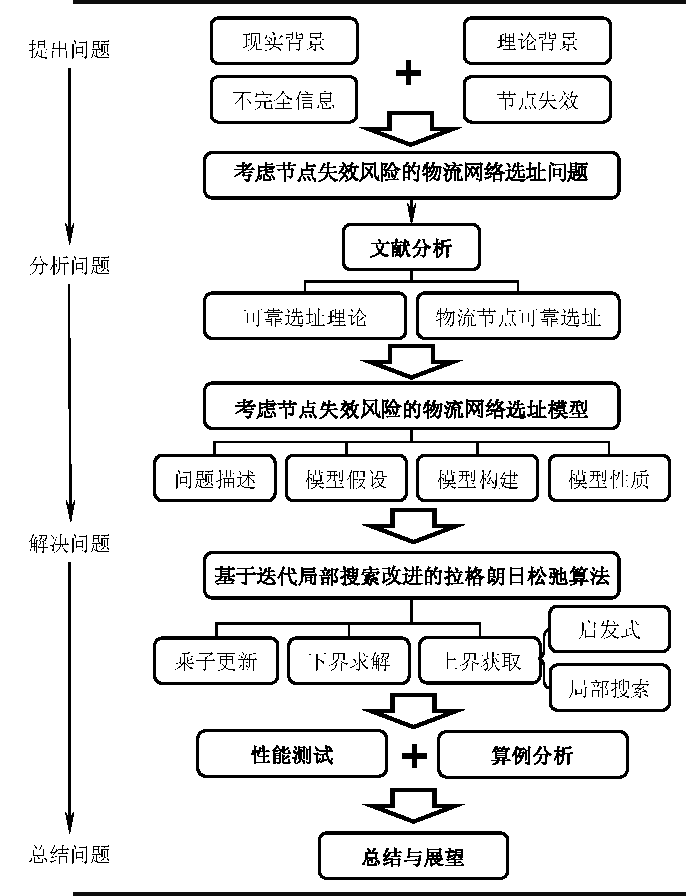
\includegraphics[height=0.7\textheight]{figures/route_.pdf}
  \caption{技术路线 \\Fig~\ref{fig:技术路线}~Technical Route}
  \label{fig:技术路线}
\end{figure}

第\ref{cha:intro}章介绍了本文的研究背景,
从繁荣发展的物流行业背后仍存在节点失效的现象出发,
引出本文的研究主题。
结合研究背景,从理论和现实两个方面明确了本文的研究意义;
分别从模型与算法两个角度阐明本文的创新性;
确定了本文的研究路线和文章结构安排。

第\ref{cha:review}章首先回顾并总结了可靠选址理论的发展过程,
着重总结了一系列建模考虑的因素和求解模型的算法,
指出了研究的薄弱之处和未来可能的研究方向。
然后简要概述了可靠选址理论在物流选址问题中的应用,
特别是相关考虑因素和解决方案。

第\ref{cha:model}章为考虑节点失效风险的物流网络选址问题构建了数学模型,
并证明了该问题的NP-hard属性。
由于该模型属于混合整数规划(Mixed Integer Programming, MIP)类型,
且带有二次约束和二次目标项,
第\ref{cha:model}章中应用了线性化技术消除模型的二次成分。
此外,模型性质分析中还讨论了一个子问题,
本文称为试错序列问题,该问题是基本最短路问题更为广泛的形式之一。

第\ref{cha:LR算法}章开发了基于迭代局部搜索改进的拉格朗日松弛算法,
从一个一般问题出发推导算法的基本原理,
并开发了一系列求解上界、下界的精确方法和启发式方法,
详细阐述了算法的控制流程。

第\ref{cha:算法性能章}章采用经典测试数据集验证了算法的性能和有效性,
对比了算法与商业求解器之间的性能差异,
分析了算法中重要算子的性能。
并对算例数据中的重要参数
进行了参数灵敏度分析,从分析结果中给出管理学启示。

第\ref{cha:summary}章总结了全文,指出本文研究工作的不足和待完善之处,
并展望了该问题未来的研究方向和研究内容。


\section{本章小结} % 1.2
\label{sec:引言小结}
本章确定了考虑节点失效风险的物流网络选址问题的研究背景,
通过现实案例介绍了物流节点所面临的失效风险以及客户的试错策略。
此外,本章介绍了研究的理论意义和现实意义以及模型和算法的创新性。
最后,确定了本文的研究思路和文章架构。
在讨论的过程中,明确了本文研究的问题基于可靠选址问题。
因此,第\ref{cha:review}章回顾了可靠选址问题相关的研究,
特别是与物流节点选址相关的文献。
                % 第一章
 \setlength{\baselineskip}{20pt}
\chapter{文献综述}
\label{cha:review}

选址问题是一个经典的优化问题。
该问题可追溯至Alfred Weber\cite{weber}于1909年首次提出的一个完善且成熟的工业选址理论,
该理论试图以最低成本找到工厂的最佳位置。
经过一个世纪的发展,已形成了一系列的经典选址模型。
基于需求和设施空间分布,
这些选址模型可分为解析选址模型、连续选址模型、网络选址模型和离散选址模型。
本文讨论的物流节点可靠选址问题属于离散选址问题,
而有关于上述四种模型的区别,
请参考Daskin的著作\cite{Daskin书}。
本章的第\ref{section:可靠选址概述}节回顾了可靠选址的发展历程,
总结了相关研究工作。
第\ref{section:节点选址概述}节描述了物流节点可靠选址理论研究现状,
指出当前研究的进展、考虑因素和解决方案。

\tinytodo[inline]{一般顺序应该是先写普通选址问题研究,
然后过渡到可靠选址理论研究;所以你的2.1和2.1 原因?
如果是后面针对物流节点选址,而2.1 是普通选址,可以从题目中进行区分。 
例如 普适性可靠选址理论综述,
物流节点选址理论综述。\newline 
\newline
\textbf{已修正}:\newline
\textbf{标题}:2.1 可靠选址理论综述 \& 2.2 物流节点可靠选址理论综述
第一段写的是可靠选址理论综述,
第二段写的是与物流相关的可靠选址综述。

\textbf{内容}:第一段由普通选址理论引出可靠选址理论。
}

\section{可靠选址理论综述}
\label{section:可靠选址概述}

\added[id=yrf]{
    离散选址问题是指
    给定一个网络拓扑结构,
    在设施候选建设位置集合中寻找满足条件的最佳子集。
    UFL问题和P-中值问题是离散选址问题的重要分支,
    二者的共同点是在网络中以最小的成本为设施选择建设的最佳位置并服务所有客户\cite{Daskin书},
    区别在于P-中值问题指定了设施选址的数量为P,
    而UFL选址问题对设施数量没有限制。
    Mak\cite{maxshen}及Daskin\cite{Daskin书}对P-中值问题和UFL选址问题的基础理论进行了详细阐述。
    本世纪初,学者们逐渐意识到不确定因素对设施网络的冲击和影响,开始着重研究节点选址中的不确定因素。
    考虑节点失效风险的选址问题起源于对供应链的中断现象的研究\cite{周愉峰综述},
    基于上述的UFL问题和P-中值问题,
    Snyder等人\cite{Snyder2005}提出了这两种选址理论的可靠版本:
    可靠P-中值问题(Reliable P-Median Problem, RPMP)和可靠无容量固定费用选址问题(RUFL)。
    可靠选址理论在经典选址模型的基础上,
    考虑每个设施损坏的概率,并为每个客户安排一个常用设施和多级备用设施,
    极大地提高了网络的可靠性。
    % 这种方法极大地提升网络的可靠性。
}

\deleted[id=yrf]{
    可靠选址理论研究是在Snyder等人\cite{Snyder2005}
    提出可靠P中值问题和可靠无容量限制设施选址问题之后开展的。
    该研究基于P-中值问题(P-median Problem, PMP)和UFL理论提出了这两种选址理论的可靠版本:
    可靠P-中值问题(Reliable P-Median Problem, RPMP)和可靠无容量固定费用选址问题(RUFL)。
    P-中值问题和无容量固定费用选址问题的共同点是在网络中以最小的成本为设施选址并服务所有客户\cite{Daskin书},
    区别在于P-中值问题指定了设施选址的数量为P,
    而UFL选址问题对设施数量没有限制。
    Mak\cite{maxshen}及Daskin\cite{Daskin书}对P-中值问题和UFL选址问题的基础理论进行了详细阐述。
    可靠选址问题的理论在经典选址模型的基础上,
    考虑每个设施损坏的概率,并为每个客户安排一个常用设施和多级备用设施。
}
Snyder\cite{Snyder2005}在其可靠选址基础理论中,
将设施分为完全可靠类型(即永久不会失效)和不完全可靠类型,
在后续研究中该理念仍被采纳\cite{rpmp,lim,李汉卿},
但大部分学者将所有设施都认定为不完全可靠状态,
即每个设施都有可能失效。
在Snyder\cite{Snyder2005}的研究基础上,
Cui\cite{Cui2010}、Shen\cite{Shen2011}、王艳敏\cite{王艳敏}松弛了设施失效概率相等的假设,
即设施的失效概率不同。
Aboolian\cite{Aboolian}不仅松弛了失效概率相等的假设,
还松弛了每个客户拥有的备用设施的数量上限,
但大部分学者仍接受客户拥有有限个备用设施的约束。

在可靠选址基本理论的基础上,
更多现实因素加入模型构建中。
首先,
导致设施损坏的灾害往往也使得通讯中断,
或者使得客户对设施的状态没有准确把握,
导致造成不完全信息状态的产生。
Berman\cite{BermanIncompleteInformation}最先研究了这种状态下的设施选址问题,
\replaced[id=syc]{Yun\cite{yun2015}基于RUFL理论提出了不完全信息下的可靠选址理论。
在该研究成果的基础上,松弛了节点失效概率相等的假设\cite{yun2017},
并考虑了返程的成本\cite{YUN2020},对所研究的可靠选址理论进行了完善。}
{Yun\cite{yun2015}基于RUFL理论提出了不完全信息下的可靠选址理论。
在Yun\cite{yun2015}的研究成果的基础上,
Yun\cite{yun2017}松弛了节点失效概率相等的假设,
Yun\cite{YUN2020}考虑了返程的成本。} 
考虑到设施可在失效之前被强化的可能,
Li等人\cite{qingwei,qingwei2,qingwei3}提出使用有限的成本强化设施,
以降低系统的总成本。
在Li\cite{qingwei2,qingwei}的研究中,
假设设施被强化后转变为完全可靠设施,
因此要求每个客户只能拥有一个常用设施和一个备用设施,
客户拥有完全可靠的设施后并不需要其余备用设施。
除了增加预算抵抗设施的失效,
风险规避也是提升可靠性的方法之一。
Yu\cite{risk_averse1,risk_averse2}提出了风险规避型可靠选址理论。
在以往的理论中,通常计算整个网络的最小期望成本,
Yu\cite{risk_averse1,risk_averse2}则控制每个客户承担的风险。
设施的失效可以是独立的,也可以是关联的,
该研究可以得到比传统模型更可靠的网络结构。

经典的RUFL理论考虑了设施的损坏失效情况,
但假设设施失效是独立的。
Lu等人\cite{lu_correlated}假定设施的失效之间存在一定的关联性,
采用了鲁棒优化方法研究了给定边际失效概率条件下的最小期望成本选址方案。
鲁棒优化是研究设施失效关联性的一种方法之一,
与鲁棒优化相关的可靠选址研究还可以参见Du等人\cite{Du}设计的双层可靠P-中心网络结构,
Peng等人\cite{peng}研究了考虑节点失效的物流网络结构,
Li等人\cite{Yongzhen}、An等人\cite{an2014reliable}提出了两阶段鲁棒优化可靠选址理论。
另一种研究失效相关的方法是连续近似模型,
Li\cite{Lixiapeng2010}构建了节点失效的关联性公式,
优化的目标是得到期望总成本最小的选址方案。
有关可靠选址的连续近似模型相关的讨论,
可见参考文献\cite{yun2019,fan,Cui2010}。
除了设施失效可能存在关联,
设施之间的相关性也可以体现在共同应对风险\cite{jiang},
使用更复杂的网络支撑结构提高整个网络的强度\cite{LiXP2013}。

上述的选址模型通过考虑设施失效的概率或边际失效概率以量化失效风险。
Berman\cite{BermanDist}将设施的可靠性与客户之间的距离关联,
研究了相关可靠选址问题。
此外,在现实中,不确定性还体现在多个方面,
例如需求不确定性的可靠设施选址\cite{cheng},
估计设施失效概率的误差\cite{lim2013facility}。
Snyder\cite{Snyder2006综述}概括了设施选址中的不确定因素,
Snyder\cite{SnyderReview}近期分析了供应链中的不确定因素,
Govindan\cite{Govindan}调查了供应链网络设计中的不确定因素。
这些研究表明,考虑不确定因素的影响是至关重要的,
可从供应链设计中借鉴经验并有效开展可靠设施选址研究。
周愉峰\cite{周愉峰综述}针对可靠选址理论的发展展开了详细描述,
并指出了未来的研究方向。

已知可靠选址问题是NP-hard问题\cite{Snyder2005},
这意味着当前不存在求解该问题的多项式时间算法。
因此,开发有效的求解算法是研究可靠选址的另一重点内容。
当前主流的可靠选址求解算法包含精确方法和启发式方法。
精确方法包括Branch-and-Bound, Benders分解,Branch-and-Price等方法,
启发式方法包括拉格朗日松弛
以及包括禁忌搜索、模拟退火、遗传算法等在内的元启发式方法。
通常,元启发式方法虽然不能保证求解的质量,
但可在可接受的时间内得到一个经过优化的可行解,
因此对于大规模问题,解决方法主要以启发式方法为主。

精确求解可靠选址问题的相关研究数量上相对较少,
求解方法主要以Benders分解算法为主。
有关Benders分解求解基本设施选址问题的研究可见参考文献\cite{fischetti,ortiz2019exact,wentges1996accelerating}。
Mohammad\cite{MohammadBenders}使用加速Benders分解算法求解了多层的可靠网络结构,
Azad\cite{Azad}开发了Benders分解算法解决了一个可应对节点失效的弹性供应链网络结构设计问题。
Pirniya\cite{Pirniya}使用了列生成(Colummn Generation)算法求解了可靠选址、客户分配及路径问题,
并取得了良好的效果。

而采用启发式算法求解可靠选址问题的研究相对较多。
拉格朗日松弛是一种求解整数规划问题以及混合整数规划问题的高效算法\cite{孙小玲,Hearn2009}。
对于求解最小化问题,
拉格朗日松弛不仅可以快速获得优化上界,
还提供了优于线性松弛的下界,
因此可以证明上界的质量。
拉格朗日松弛在求解选址问题方面取得了显著成就,
Geoffrion\cite{Geoffrion1974}首次使用拉格朗日松弛求解了UFL问题,
Cornuejols等人\cite{Cornuejols}首次使用拉格朗日松弛求解了P-中值问题。
拉格朗日松弛算法同样也是求解可靠设施选址问题的主流算法,
其设计过程具有灵活性,可根据问题定制。
因此即便都采用了拉格朗日松弛算法,
算法的技术细节都不尽相同。
Snyder\cite{Snyder2005}首次使用了拉格朗日松弛算法求解了RUFL问题,
后续的研究结果表明拉格朗日松弛求解RUFL问题效果显著:
Cui\cite{Cui2010}使用该算法求解了不等失效概率的可靠选址问题,
Yun\cite{yun2015}开发了拉格朗日松弛算法框架求解了不完美信息下的可靠选址问题,
Li\cite{qingwei}为考虑强化策略的可靠选址问题定制了拉格朗日松弛算法。
Yu\cite{risk_averse2}基于拉格朗日松弛框架设计了对偶分解算法求解了风险规避型可靠选址问题。

前文中提到拉格朗日松弛算法具有灵活性和实用性,
因此可将拉格朗日松弛作为算法框架,
将其他算法嵌入拉格朗日松弛算法中,
也可以将拉格朗日松弛嵌入其他算法中。
Xie\cite{xie}将列生成和局部搜索嵌入拉格朗日松弛,
研究了可靠选址路径问题。
Yu等人\cite{risk_averse1}将Branch-and-Cut算法和拉格朗日松弛算法相结合,
求解了风险规避型可靠选址问题。
此外,应用拉格朗日松弛算法求解可靠选址问题,
还可见参考文献\cite{YUN2020,qingwei2, wangjiguang},
有关拉格朗日松弛算法的介绍可见参考文献\cite{孙小玲},
有关算法原理的推导可见参考文献\cite{Fisher2004,Hearn2009}。

除了拉格朗日松弛之外,
还有学者采用其他启发式方法求解可靠选址问题,
包括Shen\cite{Shen2011}提出的近似算法和贪心算法,
Aboolian\cite{Aboolian}提出的近似方法,
以及Albareda\cite{rpmp}提出的近似流方法。
而元启发式方法也在求解大规模选址问题时展现了显著优势,
例如遗传算法\cite{Rahmani}、邻域搜索\cite{rainns}、禁忌搜索\cite{ts}、
变邻域搜索\cite{vns_ts}等。
求解可靠设施选址问题,
Peng等人\cite{peng}基于遗传算法和邻域搜索算法开发了混合元启发式方法,
Li\cite{qingwei3}开发了禁忌搜索算法,
Afify\cite{Afify}开发了进化学习算法,
王艳敏\cite{王艳敏}开发了模拟退火-粒子群算法。

综上,可靠选址问题的研究主要集中在两个方面:
其一是在构建模型时考虑各种现实因素,
以强化模型的现实意义。
从当前的研究成果来看,
大多可靠选址理论假设节点失效独立,
而有关节点失效相关联的研究成果较少。
在大多数可靠选址理论中,
节点的失效是以先验概率的形式表达的,
这对估计失效概率的精准程度有较高的要求,
有关失效概率预估误差对选址结果造成影响的研究较少。
其二是设计有效的算法求解该NP-hard问题。
以提升求解复杂模型的能力。
当前可靠选址求解算法研究的热门仍是启发式方法,
采用精确方法求解该问题的研究较为薄弱。


\section{物流节点可靠选址理论综述}
\label{section:节点选址概述}

物流节点是物流网络的构成要素,
节点的选址决策将显著影响物流系统的运行效率,
关系物流企业的经济利益。
窦志武等人\cite{窦志武}回顾了物流节点选址的方法,
包括重心法、整数规划模型法、层次分析法、数据包络分析法、模糊综合评价法等。
本文研究的物流节点可靠选址问题采用了整数规划模型法,
其他选址方法可见参考文献\cite{层次分析,重心法,数据包络分析}。

物流节点可靠选址的大部分研究关注于节点的状态,
特别是节点因某些原因不能提供服务的场景。
通常,物流节点失效状态由失效概率表示,
即该节点以某个概率值不能提供服务。
以供应链为研究对象,
王艳敏\cite{王艳敏}假设每个设施的失效概率不等,
建立了一个容量有限的供应链设施可靠选址的多目标模型;
张莹\cite{张莹}研究了供应中断风险的选址-路径问题,
考虑所有的设施均以先验概率发生失效,
多个设施也可以同时发生失效的场景;
汤罗浩\cite{汤罗浩}设计了一种可强化节点的供应链网络,
通过对节点进行保护并为需求点分配备份节点来提高供应链网络的可靠性;
王继光\cite{王继光}从供应链系统的可靠性和鲁棒性两方面研究了中断情境下的可靠选址问题,
针对随机中断和非随机中断分别提出了混合整数非线性规划模型和两阶段动态博弈模型。
以铁路建设为研究对象,
考虑了建筑材料的时效性需求,
周浩\cite{周浩}研究了铁路沿线的线状需求的物流节点连续型可靠选址问题,
获得了靠近需求线路中点的物流节点选址位置的解析解。
以区域物流为研究对象,
朱江华等人\cite{朱江华}以贵州省为案例开展物流园区可靠选址规划分析,
构建了考虑突发事件的物流园区选址与服务分配模型;
董鹏\cite{董鹏}以京津冀地区为例,
构建了信息失效情景下考虑双向行程的可靠节点连续选址模型。

而另一部分研究关注于线路的状态,
即节点和客户之间的线路发生中断从而不能向客户服务的场景。
颜高民\cite{颜高民}研究了突发事件下应急物流可靠路径搜索问题,
考虑了突发事件下路径畅通的不确定性,
构建了最短路和畅通路径综合模型,
并设计了一定规则修正路径。
李锐等人\cite{李锐}研究可靠绿色物流配送选址-路径问题的同时,
考虑了运输油耗和碳排放及配送中心和运输线路的中断,
建立物流配送网络选址-路径优化模型,
以最小总成本满足车辆路径约束。
考虑到供应网络中每条路径都存在运输中断风险,
任慧\cite{任慧}研究了多源协同供应的三级供应网络可靠选址路径集成优化问题,
在有限的设施(工厂、配送中心)能力下,
提出了运作成本和运输可靠性的双目标选址路径模型。
石褚巍等人\cite{石褚巍}研究了网络中存在节点和线路损坏不确定性的可靠物流网络,
提出了一种基于两阶段鲁棒优化的可靠物流网络设计方法。

除了节点和线路的不确定性,
需求和供应的不确定性也是研究的重点。
考虑到二次灾难可能造成应急配送中心失效以及救援过程中道路中断情况的发生,
张鹏阁\cite{张鹏阁}研究了需求不确定的应急物流选址-路径优化问题,
建立了一个包含常规型和可靠型的应急物流网络。
孙晓飞等人\cite{孙晓飞}研究了不确定环境下配送中心选址的多目标优化问题,
探讨了配送系统的可靠性。
姚琦\cite{姚琦}研究了生鲜农产品配送中心选址的问题,
考虑时间可靠度和品质可靠度对配送中心选址的影响,
运用层次分析法与模糊综合评价法建立了可靠物流配送中心选址模型。


此外,设施的失效常常与自然灾害相关联。
周愉峰\cite{周愉峰应急}等人以应急物资保障的及时性和可靠性为目标,
考虑在不同地区建立储备库的不同失灵概率,
构建了一个应急物资储备库的可靠P-中值选址模型,
并设计了一种拉格朗日松弛求解算法。
李政祥\cite{李政祥1}考虑设施的中断,
以成本和时间最小化为目标,
建立了应对灾害的应急物流多目标可靠选址模型。
李政祥\cite{李政祥2}构建了考虑设施设防及设施中断的多目标大规模地震灾害应急物资储备库的选址-分配模型,
设计了非支配解排序遗传算法(NSGA-II)以求解多目标问题。
朱建明\cite{朱建明}同时考虑设施可能的损毁情景以及设施两两之间的调度时间,
建立了可靠连通应急设施选址模型,
设计了基于遗传算法的求解方法。
于冬梅等人\cite{于冬梅}建立了中断情境下服务能力有限的可靠应急设施选址-分配多目标优化模型,
采用带精英策略的快速NSGA-II对模型予以求解。
王子墨\cite{王子墨}建立了考虑失效风险的救灾物资储备库可靠选址模型,
对储备库的位置、容量和需求点与救灾物资储备库的分配关系进行决策,
并通过遗传算法对模型进行求解。

综上,
物流节点的可靠选址研究将可靠选址理论与实际结合,
根据现实场景和需求
进一步拓展和应用可靠选址理论。
物流节点可靠选址问题的研究主要考虑了节点、线路、供应和需求的不确定性,
研究对象涵盖了供应链网络优化、物流园区设计、配送中心选址、应急物流规划等内容。


\section{本章小结}

选址问题是运筹优化领域经久不衰的一项重要研究内容,
而可靠选址研究是近二十年来选址理论的重要发展成果。
本章详细展开了可靠选址的发展过程,
介绍了可靠选址的起源以及可靠选址问题重要分支。
这些研究成果可分为理论创新和算法创新。
理论创新考虑了更多的现实因素,
而随着越来越多的现实因素加入模型中,
求解模型的困难程度提升,
也促进了相关算法的发展。

此外,可靠选址是物流节点选址的热门研究内容。
物流系统可能会面临各种不确定因素,
这些不确定因素可发生于供给端、需求端以及二者之间连接过程,
对物流网络造成严重的负面影响,
因此有必要在选址时将不确定因素考虑其中。
由本章文献综述可知,
考虑节点失效风险和不完全信息场景下客户试错策略的研究相对较少。
研究该问题有助于强化物流网络结构,
合理规划节点选址和客户分配,
为物流网络结构设计提供理论支撑。
为采用科学方法研究该问题,
本文的第\ref{cha:model}章构建了该问题的数学优化模型。







                % 第二章
\setlength{\baselineskip}{20pt}
\chapter{考虑设施失效风险的物流网络选址模型构建}
\label{cha:model}

如第\ref{cha:intro}章所述,
物流节点的运营常常伴随风险。
这些风险导致物流节点失效的同时还伴随不完全信息状态的产生。
一般情况下,节点失效的概率是先验的。
可通过包括气象、新闻在内的历史数据,
统计失效时长占总统计时长的比例获得节点的失效概率,
或统计失效次数占总次数的比例获得,
还可以通过调研对未来失效概率进行预测。
由于不同地区、不同位置的候选点的外部环境不同,
每个节点的失效概率也不相同。
根据客户的试错策略,
访问某一级备用节点的概率将与其之前访问的所有节点的失效概率相关。
为了表示这种概率关系,
\replaced[id=syc]{本章采用了非线性方法表达模型的目标函数和约束。}{本章的模型约束和目标函数采用了非线性表达。} 
同时本章提供了线性化技术处理模型中非线性成分,
降低了使用精确方法(例如商业求解器)求解模型的难度。

本章的主要内容和结构如下:
首先,第\ref{sec:suppose}节声明了模型中存在的理想化假设。
其次,第\ref{sec:description}节使用了数学语言表述了问题。
然后,第\ref{sec:model}节建立了数学模型。
此外,第\ref{sec:线性化}节提供了模型的线性化方案,
第\ref{sec:attribute}节分析了该模型的一系列性质,
证明该问题的NP-hard性质,并讨论了模型的子问题与基本最短路问题的关系。
最后,第\ref{sec:小结3}节总结了本章的内容。

\section{模型假设}
\label{sec:suppose}
本文考虑节点失效风险的物流网络选址模型
同其他数学模型一样存在一系列理想化假设。
由于本文的模型根源于UFL选址理论,
因此继承了UFL问题的一般假设:
\begin{enumerate}[label=(\arabic*),leftmargin=0pt,itemindent=3.5\ccwd, nosep]
  \item 客户的需求已知;
  \item 客户的单次需求不可拆分;
  \item 所有节点均不考虑容量限制。
\end{enumerate}
此外,
\deleted[id=yrf]{基于一般的UFL问题,}
针对本文讨论的问题的特殊性,
提出了以下的理想化假设:
\begin{enumerate}[label=(\arabic*),leftmargin=0pt,itemindent=3.5\ccwd, nosep, resume]
  \item 假设每个节点的失效概率是先验的;
  \item 节点失效发生彼此独立。
\end{enumerate}
最后,本文考虑的问题基于一般图,
因此基于图理论假设:
\begin{enumerate}[label=(\arabic*),leftmargin=0pt,itemindent=3.5\ccwd, nosep, resume]
  \item 任意两点之间的成本是非负且不可变动的;
  \item 两点之间的道路是永远联通的(即,图中弧和弧的权重不变)。
\end{enumerate}

\section{问题描述和符号说明}
\label{sec:description}
本节将使用数学语言更为严谨地描述前文所述的问题,
相关符号表示如下
(为方便索引,在本节末尾的表\ref{table:符号}给出了符号及其对照解释):
设$I$表示客户点的集合,设$J$表示候选点的集合。
给定一个有向图$G=(V,A)$,
其中$V=I \cup J$是点集,
\replaced[id=yrf]{$A=\{(i,j)|i\in V ,j \in J\}$是弧集。}{$A=\{(i,j)|i\in V ,j \in V\}$是弧集。}
每个客户$i\in I$的需求为$\lambda_i$,
每个候选点$j\in J$的建设成本为$f_j$,失效的概率为$q_j$。
每条弧$(i,j)\in A$的权重为$c_{ij}$,
表示从点$i\in V$到点$j\in J$单位需求的运输价格(本章简称为价格)。

任一客户$i\in I$可以同时拥有一个常用节点和多个备用节点,
但每个客户的备用节点数可能不同。
额外引入虚拟节点$j_0$,
并规定客户试错过程的最终节点一定为虚拟节点$j_0$\deleted[id=yrf]{,
即指定一个虚拟节点并安排在每个客户的试错策略的末尾}。
访问虚拟节点表示当客户的所有实体节点(常用节点和备用节点)都失效时接受的惩罚。
从点集$V$中的点$i \in V$到虚拟节点$j_0$的价格
$c_{ij_0},\forall i \in V$等于惩罚价格$\pi$,
表示客户用尽所有备用节点都没有获得服务后产生的损失。
虚拟节点的建设成本$f_{j_0}=0$,失效概率$q_{j_0}=0$,
定义集合$J$被$j_0$扩充后的集合记为$\bar{J} = J\cup \{j_0\}$。
此外,限制每个客户拥有的实体节点数之和小于等于$R$,表示客户可接受的最大尝试次数。

为了可视化地展示客户试错过程,以及推导期望运输成本,
图\ref{fig:trail}展示了客户的试错策略。
图中客户用正方形表示,实体节点用实体圆形表示,
虚拟节点用空心圆形表示,弧旁符号表示该段弧的价格。
图中集合$J_i = \{j_i^r|r = 0,1,...,R-1\}$为服务客户$i$的实体节点,
上标$r$表示访问的先后顺序,
即客户第$r$等级的备用节点($r=0$表示常用节点),
因此集合$J_i$中元素的个数$|J_i|$不超过$R$。

\begin{figure}[ht] % use float package if you want it here
%\setlength{\abovecaptionskip}{-0.2cm} %调整图片caption与正文之间的间距,table同理。可自己调整。
\setlength{\belowcaptionskip}{-0.5cm} 
  \centering
  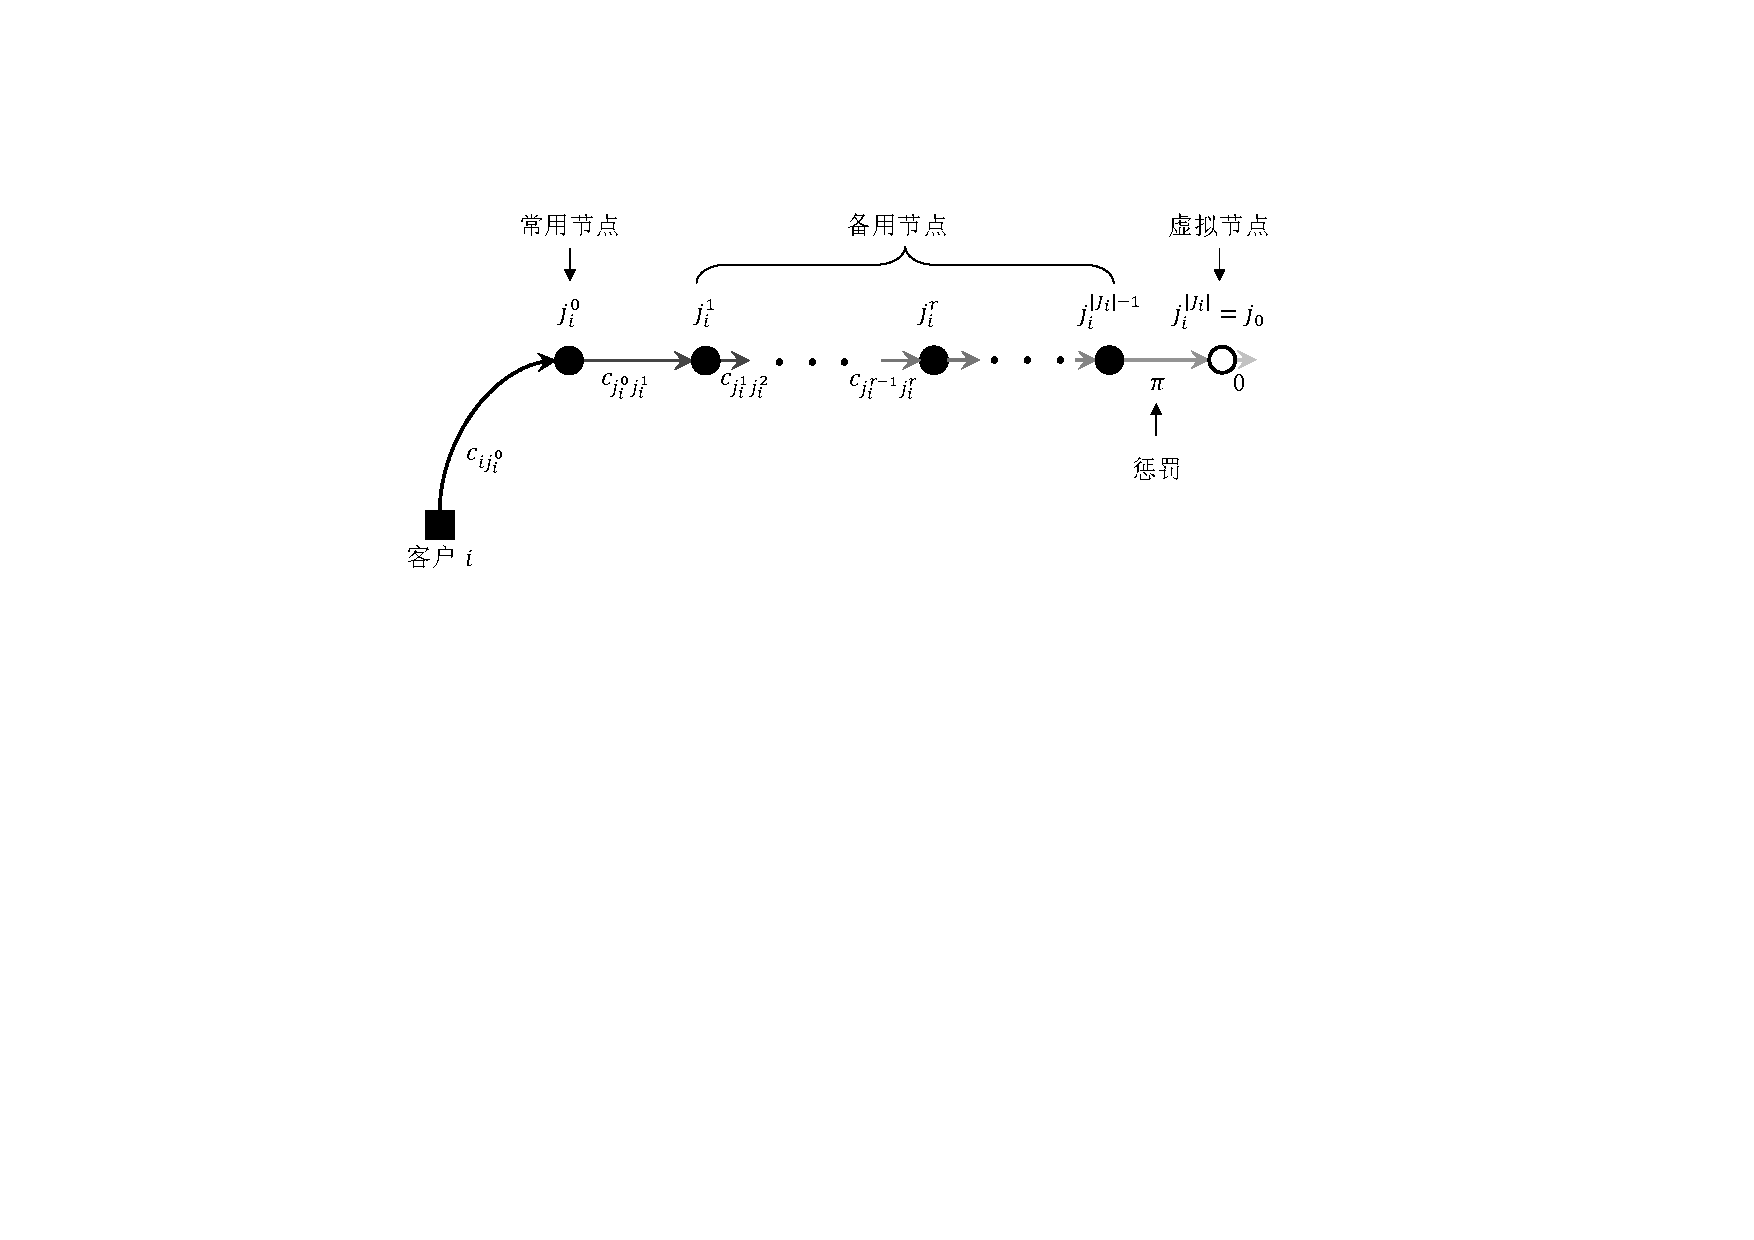
\includegraphics[width=\textwidth
    % height=\dimexpr\pagegoal-\pagetotal-4\baselineskip\relax, % 塞进本页的最后
  ]{figures/试错策略示意图.pdf}
  \caption{客户试错策略示意图\\Fig~\ref{fig:trail}~ A Trail-and-error Strategy of a Customer}
  \label{fig:trail}
\end{figure}

当客户$i$访问节点$j_i^0$时,$j_i^0$以$q_{j_i^0}$的概率失效,
以$1-q_{j_i^0}$的概率提供服务。
如果节点$j_i^0$正常服务,
那么客户$i$从节点$j_i^0$获得服务的期望成本等于$\lambda_i c_{ij_i^0} (1-q_{j_i^0})$。
如果节点$j_i^0$失效,那么客户$i$将从$j_i^0$继续出发访问节点$j_i^1$。
同样,若节点$j_i^1$正常服务,
那么客户$i$从节点$j_i^1$获得服务的期望成本等于$\lambda_i (c_{ij_i^0}+c_{j_i^0j_i^1}) q_i^0(1-q_{j_i^1})$,
即在上一个点$j_i^0$失效的情况下点$j_i^1$没有失效。
若节点$j_i^1$失效,则客户$i$将从$j_i^1$继续出发访问节点$j_i^2$,
以此类推,直至客户接受服务或访问完所有节点。

归纳上述推导过程,客户$i$访问第$r(r\ge 1)$等级的节点的期望成本$C_e^{ir}$,
如公式(\ref{eq:expectcost})所示:
\begin{equation}
\label{eq:expectcost}
C_e^{ir}=\lambda_i 
\left( 
c_{ij_i^0}+ \sum_{m=1}^r c_{j_i^{m-1} j_i^{m}}
\right)
\left( 
\prod_{n=0}^{r-1} q_{j_i^n}-\prod_{n=0}^{r} q_{j_i^n}
\right)
\end{equation}
于是,对所有等级$r$求和,
客户$i$的总期望成本$C_t^i$如公式(\ref{eq:sumcost})所示:
\begin{equation}
\label{eq:sumcost}
C_t^i = \lambda_i \sum_{r=1}^R
\left( 
(c_{ij_i^0}+ \sum_{m=1}^r c_{j_i^{m-1} j_i^{m}})
(\prod_{n=0}^{r-1} q_{j_i^n}-\prod_{n=0}^{r} q_{j_i^n})
\right) +
\lambda_i c_{ij_i^0} (1-q_{j_i^0})
\end{equation}
公式(\ref{eq:sumcost})等号右侧的第一项表示从$r=1$至$r=R$的期望运输成本之和,
右侧第二项表示虚拟节点的期望惩罚成本。
提取前面的一个求和项$r=1$与后面的项合并得到,
\begin{equation}
\begin{aligned}
C_t^i &= \lambda_i \sum_{r=2}^R
\left( 
(c_{ij_i^0}+ \sum_{m=1}^r c_{j_i^{m-1} j_i^{m}})
(\prod_{n=0}^{r-1} q_{j_i^n}-\prod_{n=0}^{r} q_{j_i^n})
\right) \\
& - \lambda_i(\prod_{n=0}^1 q_{j_i^n})(c_{ij_i^0} + \sum_{m=1}^1 c_{j_i^{m-1}j_i^m})\\
& + \lambda_i(c_{ij_i^0} + c_{j_i^{0}j_i^{1}} \prod_{n=0}^0q_{j_i^n})
\end{aligned}
\end{equation}
再提取一项$r=2$与后面的项合并,得到,
\begin{equation}
\begin{aligned}
C_t^i &= \lambda_i \sum_{r=3}^R
\left( 
(c_{ij_i^0}+ \sum_{m=1}^r c_{j_i^{m-1} j_i^{m}})
(\prod_{n=0}^{r-1} q_{j_i^n}-\prod_{n=0}^{r} q_{j_i^n})
\right) \\
& - \lambda_i(\prod_{n=0}^2 q_{j_i^n})(c_{ij_i^0} + \sum_{m=1}^2 c_{j_i^{m-1}j_i^m})\\
& + \lambda_i(c_{ij_i^0} + c_{j_i^{0}j_i^{1}} \prod_{n=0}^0q_{j_i^n} + c_{j_i^{1}j_i^{2}} \prod_{n=0}^1q_{j_i^n})
\end{aligned}
\end{equation}
如此进行,直至全部展开,最终得到,
\begin{equation}
\label{eq:sumcostlast}
\begin{aligned}
C_t^i &= - \lambda_i(\prod_{n=0}^{R} q_{j_i^n})(c_{ij_i^0} + \sum_{m=1}^{R} c_{j_i^{m-1}j_i^m})\\
& + \lambda_i(c_{ij_i^0} + c_{j_i^{0}j_i^{1}} \prod_{n=0}^0q_{j_i^n} + 
 c_{j_i^{1}j_i^{2}} \prod_{n=0}^1q_{j_i^n} + ...
+ c_{j_i^{R-1}j_i^{R}} \prod_{n=0}^{R-1}q_{j_i^n})
\end{aligned}
\end{equation}
由于设定$r=R$时,备用节点一定为虚拟节点,
于是有$q_{j_i^R} = q_{j_0} = 0$,
所以公式(\ref{eq:sumcostlast})的负数项可消除($\prod_{n=0}^{R} q_{j_i^n}=0$),
后面的正数项经过整理,可表示为,
\begin{equation}
\label{eq:sumcostabbr}
C_t^i = \lambda_i
\left( 
    c_{ij_{i}^0} + \sum_{r=1}^R c_{j_i^{r-1}j_i^{r}}(\prod_{n=0}^{r-1} q_{j_i^n})
\right)
\end{equation}
公式(\ref{eq:sumcostabbr})得到了一个客户$i\in I$的期望运输成本,
所有客户的期望运输成本等于:
\begin{equation}
C_t = \sum_{i\in I}\lambda_i
\left( 
    c_{ij_{i}^0} + \sum_{r=1}^R c_{j_i^{r-1}j_i^{r}}(\prod_{n=0}^{r-1} q_{j_i^n})
\right)
\end{equation}

至此,关于客户的期望运输成本的推导已完成。
考虑节点失效风险的物流网络选址问题可正式定义为:
给定一个客户集$I$和节点候选拓展集$\bar{J}$,
以及弧的权重$\{c_{ij}|\forall i \in I\cup \bar{J},\forall j\in \bar{J}\}$,
节点的损坏概率$q_j,\forall j\in \bar{J}$、建设成本$f_j,\forall j\in \bar{J}$,
客户的需求$\lambda_i,\forall i \in I$,
求一个子集$J^*\subseteq \bar{J}$以及每个客户$i$访问子集$J_i^*\subseteq J^*$的序列$s_i = (j_i^0,...,j_i^r,...,j_i^R),\forall j_i^r \in J_i^*,\forall i\in I, r=0,...,R$,
使得建设节点的固定成本$C_f=\sum_{j\in J^*}f_j$与客户的期望运输成本$C_t=\sum_{i\in I}\lambda_i
\left( c_{ij_{i}^0} + \sum_{r=1}^R c_{j_i^{r-1}j_i^{r}}(\prod_{n=0}^{r-1} q_{j_i^n})\right)$之和最小。

最后,建模过程用到的所有符号定义如表\ref{table:符号}所示:

\begin{table}[!htb]\normalsize   %%\small是为了设置表格中的字体比正文小
\setlength{\abovecaptionskip}{-0.05cm} %调整图片caption与正文之间的间距,table同理。可自己调整。
\setlength{\belowcaptionskip}{-0.2cm} 
  \centering
  \renewcommand\arraystretch{1}
  \caption{符号释义表\\Table~\ref{table:符号}~Notation List}
\begin{tabular}{p{1.5cm}<{\centering} l}
 % \begin{tabular}{c}{l}
  \toprule
  \textbf{符号} & \textbf{解释} \\
  \midrule %[2pt]
    $G$   &  有向图      \\
    $V$   &  图$G$的点集      \\
    $A$   &  图$G$的弧集      \\
    $I$   &  客户点集 \\
    $J$   &  候选点集 \\
    $\lambda_i$ & 客户$i\in I$的需求 \\ 
    $f_j$   &  节点$j\in J$的建设成本 \\
    $q_j$   &  节点$j\in J$的失效概率 \\
    $c_{ij}$ & 弧$(i,j)$的权重 \\
    $\pi$ & 惩罚价格 \\
    $j_0$ & 虚拟节点 \\
    $R$ & 每个客户备用节点的最大个数 \\
    $\bar{J}$ & 集合$J$与\{$j_0$\}的并集 \\
    $r$ & 备用节点的等级 \\
    $j_i^r$ & 客户$i$的第$r$等级的节点 \\
    $C_e^{ir}$ & 客户$i$访问第$r$等级备用节点的期望成本 \\
    $C_t^i$ & 客户$i$的总期望运输成本 \\
    $C_t$   & 总期望运输成本 \\
    $C_f$   & 总建设成本 \\
    $J_j^+$ & 可在$j$之前访问的节点集合\\
    $J_j^-$ & 可在$j$之后访问的节点集合\\
    % $y_j$    & 决策变量,决定是否建设节点\\
    % $z_{ij}$ & 决策变量,决定客户的常用节点\\
    % $x_{ijj'r}$ & 决策变量,客户的试错策略\\
    % $p_{ijj'r}$ & 中间变量,记录概率关系\\
    % $w_{ijj'r}$ & 辅助变量,线性化目标函数和约束\\
  \bottomrule
  \end{tabular}
  \label{table:符号}
\end{table}

\section{模型构建}
\label{sec:model}
本节将构建考虑节点失效风险的物流网络选址问题的非线性混合整数规划模型,
该模型的目标函数为最小化总成本,
包括建设节点的固定成本(投资成本)和客户的期望运输成本,
其中期望运输成本的计算过程已在\ref{sec:description}节推导。
第\ref{subsec:obj}节明确了模型的目标函数,
第\ref{subsec:st}节描述了模型的约束。

\subsection{目标函数推导}
\label{subsec:obj}
本小节将构建模型的目标函数,
关于问题描述中符号的定义参见表\ref{table:符号}。
在定义决策变量之前,
为了表达客户访问节点的先后顺序,
本章将采用两点之间是否存在弧的方法表示客户的试错方案。
使用这种``弧''的概念借鉴了车辆路径问题(Vehicle Routing Problem, VRP)的决策变量处理思路\cite{vigo}
以及Albareda等人\cite{rpmp}研究可靠P-中值问题对决策变量的处理。

由于每个客户从自身位置出发,因而起点不同。
定义集合$J_{ij}^+$和集合$J_{ij}^-$分别表示客户$i$在点$j$之前和之后可访问的点集,
\added[id=yrf]{公式如下:}
\begin{equation}
    J_{ij}^+ =
    \begin{cases}
        \{i\} \cup J \backslash \{j\} & \text{ if } j \ne j_0\\
        \{i\} \cup J                  & \text{ if } j = j_0
    \end{cases},
    \forall i \in I, j\in J
    \label{eq:after}
\end{equation}

\begin{equation}
J_{ij}^- =
\begin{cases}
\bar{J} \backslash \{j\} & \text{ if } j \ne i\\
\bar{J}                  & \text{ if } j = i
\end{cases},
\forall i \in I, j\in J
\label{eq:before}
\end{equation}

上述公式(\ref{eq:after})和公式(\ref{eq:before})可解释为:
对于客户$i$,只能从客户点$i$以及不包括节点$j$自身的任意实体节点访问节点$j$,
但可从客户点$i$以及任意实体节点访问虚拟节点$j_0$。
同理,对于客户$i$,客户从$i$出发后可以访问任意节点,
但是访问节点$j$之后访问的下一个点不能再是节点$j$。

该模型共需要两种决策变量和一种中间变量,
具体定义如下:
\begin{enumerate}[label=(\arabic*),leftmargin=0pt,itemindent=3.5\ccwd, nosep]
\item $y_j,\forall j \in J$:
选址0-1决策变量,等于1表示在候选节点$j\in J$处建设节点,
等于0表示不在该处建设。

\item $x_{ijk},\forall i \in I, j \in J\cup \{i\}, k\in J_{ij}^-$:
试错序列0-1决策变量,等于1表示弧$(j,k)$属于客户$i$,
等于0表示弧$(j,k)$不属于客户$i$。

\item $p_{ijk},\forall i \in I, j \in J\cup \{i\}, k\in J_{ij}^-$:
概率连续中间变量,上界等于1下界等于0,
表示客户$i$从节点$j$访问节点$k$的概率。
\end{enumerate}

模型的目标函数是最小化总成本,
包含建设节点的固定成本以及期望运营成本,
具体如公式(\ref{eq:obj})所示。
\begin{equation}
\label{eq:obj}
\min C = \sum_{j\in J}f_jy_j
+ \sum_{i\in I}\lambda_i 
\sum_{k\in J_{ij}^+}\sum_{j\in \bar{J}}
c_{kj} p_{ikj} x_{ikj}
\end{equation}

公式(\ref{eq:obj})的
第一部分计算了建设节点的成本,第二部分计算了期望运输成本。
目标函数中期望运输成本是在公式(\ref{eq:sumcostabbr})的基础上引入决策变量构成的。
公式(\ref{eq:sumcostabbr})的累乘项$\prod_{n=0}^{r-1} q_{j_i^n}$被中间变量$p_{ikj}$替换。
关于$p_{ikj}$的递推关系,
详见约束(\ref{eq:st_probinit})和约束(\ref{eq:st_probmiddle})。
值得注意的是决策变量$x_{ikj}$和中间变量$p_{ikj}$相乘,
因此该目标函数是非线性(二次)的。

\subsection{数学模型}
\label{subsec:st}
考虑节点失效风险的物流网络选址模型如下:
\begin{equation}
\label{eq:obj_model}
\min C = \sum_{j\in J}f_jy_j + \sum_{i\in I}\lambda_i \sum_{k\in J_{ij}^+}\sum_{j\in \bar{J}} c_{kj} p_{ikj} x_{ikj}
\end{equation}
\textit{s.t.}
\begin{gather}
% 指定给开启的节点
\sum_{k\in J_{ij}^+}x_{ikj} \le y_j ,\forall i \in I , j\in J \label{eq:st_assign2open}\\
% 流开始与结束
\sum_{j\in J_{ii}^-}x_{iij} = \sum_{j\in J_{i{j_{0}}}^+} x_{ijj_0} = 1, \forall i \in I  \label{eq:st_flow}\\
% 流平衡
\sum_{k\in J_{ij}^-} x_{ijk} = \sum_{k\in J_{ij}^+} x_{ikj}, \forall i \in I, j \in J \label{eq:st_flowbalance}\\
% 概率初始化
p_{iij} = x_{iij}, \forall i\in I, j\in J_{ii}^- \label{eq:st_probinit}\\
% 概率递推
q_j\sum_{k\in J_{ij}^+} x_{ikj} p_{ikj}= p_{ijj'}, \forall i \in I, j \in J, j'\in J_{ij}^- \label{eq:st_probmiddle} \\
% 尝试次数
\sum_{j\in J\cup\{i\}} \sum_{k\in J_{ij}^-} x_{ijk} \le R, \forall i\in I \label{eq:st_trytimes} \\
% y决策
y_{j} \in\{0,1\}, \forall j \in {J} \label{eq:st_y}\\
% x决策
x_{ijk} \in \{0,1\}, \forall i \in I, j \in J\cup \{i\}, k\in J_{ij}^- \label{eq:st_x}\\
% p决策
0 \le p_{ijk} \le 1, \forall i \in I, j \in J\cup \{i\}, k\in J_{ij}^- \label{eq:st_p}
\end{gather}

目标函数(\ref{eq:obj_model})表示最小化总成本。
约束(\ref{eq:st_assign2open})规定只有已建设的备用节点才有可能成为某个客户的常用或备用节点;
约束(\ref{eq:st_flow})表示客户出发点和终点的流平衡约束,客户必须出发前往某个节点,也必须从某个点到达虚拟节点(终点);
约束(\ref{eq:st_flowbalance})是中间点的流平衡约束,规定进入节点的流量等于流出节点的流量;
约束(\ref{eq:st_probinit})初始化每个客户出发对应弧的概率;
约束(\ref{eq:st_probmiddle})表达了两段相邻弧的概率递推关系;
约束(\ref{eq:st_trytimes})限制了每个客户尝试的次数,即每个客户拥有的弧的个数;
最后,约束(\ref{eq:st_y})和(\ref{eq:st_x})是决策变量0-1整数约束,约束(\ref{eq:st_p})表示中间变量的上下界。

\section{模型线性化}
\label{sec:线性化}
由于第\ref{sec:model}节给出的数学模型是非线性混合整数规划模型,
本小节针对该模型提出了降低模型复杂程度的线性化方法。
模型中的非线性的部分,
分别出现在目标函数(\ref{eq:obj})和约束(\ref{eq:st_probmiddle})中。
采用等价替换方法消除模型中的二次项,
令$w_{ijk} = p_{ijk}x_{ijk},\forall i \in I, j \in J\cup \{i\}, k\in J_{ij}^-$,则目标函数(\ref{eq:obj_model})可替换为,
\begin{equation}
\min C = \sum_{j\in J}f_jy_j + \sum_{i\in I}\lambda_i \sum_{k\in J_{ij}^+}\sum_{j\in \bar{J}} c_{kj} w_{ikj}
\end{equation}
使用相同的方式,替换约束(\ref{eq:st_probmiddle})中的非线性部分,
则约束(\ref{eq:st_probmiddle})变为,
\begin{equation}
q_j\sum_{k\in J_{ij}^+} w_{ikj}= p_{ijj'}, \forall i \in I, j \in J, j'\in J_{ij}^- \label{eq:l_st_probmiddle} \\
\end{equation}
需注意,当前的替换并不是等价的。
$w_{ijk}, \forall i \in I, j \in J, j'\in J_{ij}^-$作为中间变量,在替换时需补充一些等价约束,这些等价约束限制了中间变量的取值范围,保证替换的等价性。
注意到变量$x_{ijk},\forall i \in I, j \in J, k\in J_{ij}^-$为0-1约束,
变量$p_{ijk},\forall i \in I, j \in J, k\in J_{ij}^-$为[0,1]之间的连续变量。
由于$w_{ijk},\forall i \in I, j \in J, k\in J_{ij}^-$等于对应变量相乘,
那么$w_{ijk}$的上界将取二者的较小值,下界将大于二者之和减1,即等价约束如下:
\begin{gather}
% 上界1
w_{ijk} \le p_{ijk}, \forall i \in I, j \in J \cup \{i\}, j'\in J_{ij}^- \\
% 上界2
w_{ijk} \le x_{ijk}, \forall i \in I, j \in J \cup \{i\}, j'\in J_{ij}^- \\
% 下界
w_{ijk} \ge p_{ijk} + x_{ijk} - 1, \forall i \in I, j \in J \cup \{i\}, j'\in J_{ij}^-\\
% 范围
0 \le w_{ijk} \le 1, \forall i \in I, j \in J \cup \{i\}, j'\in J_{ij}^- \label{eq:st_w}
\end{gather}

% 考虑节点失效风险的物流网络选址模型及算法研究
考虑节点失效风险的物流网络选址模型的线性化版本如下:
\begin{equation}
\label{eq:l_obj_model}
\min C = \sum_{j\in J}f_jy_j + \sum_{i\in I}\lambda_i \sum_{k\in J_{ij}^+}\sum_{j\in \bar{J}} c_{kj} w_{ikj}
\end{equation}
\textit{s.t.}
\begin{center}
    约束(\ref{eq:st_assign2open}) - 约束(\ref{eq:st_probinit}) \\
    约束(\ref{eq:st_trytimes}) - 约束(\ref{eq:st_p}) \\
    约束(\ref{eq:l_st_probmiddle}) - 约束(\ref{eq:st_w})
\end{center}

\section{模型性质}
\label{sec:attribute}
% 考虑节点失效风险的物流网络选址模型及算法研究
本节将对考虑节点失效风险的物流网络选址数学模型进行一系列性质分析。
首先,第\ref{subsec:nph}小节简要说明了复杂度理论,
并证明了该模型的NP-hard性质,
其次,第\ref{subsec:subprob}小节提出了该问题的一个子问题,
在本文中称为试错序列问题,
该问题是基本最短路问题更一般的形式。

\subsection{NP-hard}
\label{subsec:nph}
根据复杂度理论,如果一个问题如果能在多项式时间(Polynomial time)内求解,
那么这个问题归类为P问题(Polynomial Problem)。
如果一个问题可以在多项式时间内验证解的正确性,
那么这个问题是非确定性多项式时间问题
(Nondeterministic Polynomial-time Problem)即NP问题。
其中,``非确定性''是指不知道这个解是怎样获得的,且很有可能是猜测的。

显然,P问题是NP问题的子集,因为在多项式时间内能解决的问题,
一定能在多项式时间内验证解的正确性。
但是P问题是否等于NP问题至今没有准确的结论。

在NP问题中,有一类问题称为NP完全问题或NPC问题
(Nondeterministic Polynomial-time Complete Problem)。
当一个问题是NP问题,且所有的NP问题都能多项式归约至这个问题时,
那么这个问题是NPC问题。
这说明NPC问题可以相互多项式归约转化。
如果NPC问题存在多项式时间解法,
则说明所有的NP问题都能在多项式时间内解决,那么就证明了P=NP问题。
当前研究已为一些NPC问题找到了伪多项式时间
(Pseudo Polynomial-time algorithm)算法(
时间复杂度是问题规模的多项式,空间复杂度是问题规模的非多项式),
这类问题称为弱NPC问题,另一类不存在伪多项式时间算法的NPC问题称为强NPC问题。

当一个问题满足``所有的NP问题都能多项式归约至这个问题''的条件时,
那么这个问题称为NP-hard问题(Nondeterministic Polynomial-time Hard Problem)。
这说明NP-hard问题目前没有多项式时间算法,也说明NPC问题属于NP-hard问题。

在简单介绍完复杂度理论后,
接下来将证明考虑节点失效风险的物流网络选址问题是NP-hard问题。
本节将从集合覆盖问题逐步推导至UFL问题,再推导至本文研究的问题。
集合覆盖问题是指一类经典的组合优化问题,
该问题的决定性版本(即,回答为``是''或``否''的问题,例如有一个问题的解,判断其是否为最优解)
是Karp\cite{karp}定义的经典21个NPC问题之一,
其优化版本(即,找到该问题最优解的优化过程)是NP-hard问题。
集合覆盖问题是指给定一个全集$U$包含$m$个元素,
集合$S$中包含了$n$个集合且这$n$个集合的并集等于$U$,
$S=\{ S_1, S_2, ..., S_n\}, \bigcup_{i = 1,...,n}S_i = U$。
在$S$中寻找一个最小的子集,使该子集的并集等于$U$。
关于引理的证明可参考Garey等人\cite{garey1979computers}
对于NPC问题与复杂度理论的详细论述。
证明集合覆盖问题是NPC问题超过了本文的范畴,
因此本文不再复述其具体的证明过程,而直接将其作为引理使用。

\begin{description}[leftmargin=0pt, topsep=0pt, parsep=0pt]
  \item[引理 1] 集合覆盖问题的决定性版本是NPC问题,优化版本是一个NP-hard问题。
  \item[推论 1] 无容量限制固定费用选址问题(UFL)是NP-hard问题。
  \item[证明 1] 关于UFL问题论述所用的符号直接沿用了第\ref{sec:description}节的定义。
  基于集合覆盖问题的定义(符号同样沿用),
  做一个辅助图$H$,$H$分为左右两个部分。
  对于左部分,若存在一个元素$u\in U$,则左侧增加一个点$h_u$。
  对于右部分,若存在一个子集$S_k \subseteq \{h_1, h_2, ... , h_m\}$,
  则在右侧增加一个点$S_k$,子集数量上限为$n$。
  如果$h_u \in S_k $,则存在一条边$e_{h_uS_k}$。
  图$H$构建完成后,将在该图上进一步考虑一个UFL问题。
  令点集$I:=\{h_1, h_2, ... ,h_m\}$表示客户点,
  点集$J:=\{S_1, S_2,...,S_n\}$表示候选节点。
  令UFL问题中,固定成本为1,即$f_j=1$,
  若边$e_{h_uS_k}$存在,则$c_{h_uS_k}=0$。这样,一个UFL问题变为以最少的节点数($H$中右侧)使得每个客户($h_u$)可以被与之相连的节点($S_k$,且$S_k$包含$h_u$)服务。
  该UFL问题就转换成了一个集合覆盖问题。
  显然,当且仅当集合覆盖问题取最优时,这个特殊的UFL问题取最优。
\end{description}

上述的转换过程,称为多项式归约。
它使得一个UFL问题转换成一个已知的NP-hard问题,
进而证明了UFL问题是一个NP-hard问题。
从UFL问题出发,
可推导考虑节点失效风险的物流网络选址问题是NP-hard问题。

\begin{description}[leftmargin=0pt, topsep=0pt, parsep=0pt]
  \item[推论 2] 考虑节点失效风险的物流网络选址问题是NP-hard问题。
  \item[证明 2] 在第\ref{sec:model}节构建的模型中,
  令R=1,则每个客户只有一个常用节点可以使用,无可用的实体备用节点。
  由于常用节点的失效概率已知,则相关价格的期望值也已知。
  那么该问题退化成一个UFL问题,并且由推论1可知UFL问题是NP-hard问题,
  那么未退化的原问题也是NP-hard问题。
  换句话说,该问题拓展了UFL问题,进而也是NP-hard问题。
  该证明详情可参考Li\cite{qingwei}等人的研究。
\end{description}


\subsection{子问题:试错序列问题}
\label{subsec:subprob}
根据客户的试错策略,
本文提出了考虑节点失效风险的物流网络选址问题的一个子问题,
本文称作试错序列问题,
是指在给定已建成的节点集合$J^*$中,
为每个客户指派一条期望成本最低的试错序列。
研究试错序列问题的解法可以带来两方面的好处。
首先,当求解主问题的启发式算法给出了节点选址方案时,
快速求解试错序列问题可以提升评估方案质量的效率。
其次,假设所有的节点均可用并增加访问节点的一项固定成本时,
该问题则是主问题的拉格朗日松弛形式,
这将在第\ref{cha:LR算法}章中介绍。

该问题的正式定义如下:
给定已建设的节点集合$J^*$,客户集合$I$,虚拟节点$j_0$
以及弧的权重$\{c_{ij}|\forall i \in I\cup J^*,\forall j\in J^*\}$,
节点的损坏概率$q_j,j\in J^*$,
客户的需求$\lambda_i,\forall i \in I$,
每个客户最大尝试次数$R$,
对于每个客户$i\in I$来说,求从$i$出发访问$J^*$中的节点,
并前往$j_0$的总期望运输成本最小的序列,
并且该序列的中虚拟节点和已建设节点的总数不超过$R$。
图\ref{fig:trail}展示了这种试错序列的起点与终点定义,
此外,期望运输成本的计算方法参见公式(\ref{eq:sumcostabbr})。
同样,本节给出试错序列问题一般形式的数学模型,
为了方便表述,
该模型使用的符号继承表\ref{table:符号}的定义。
不失一般性地假设$J^* = J$,即所有的设施均被建设。
给定一个客户点$i\in I$,
定义0-1决策变量$z_{kj}, \forall j \in \bar{J}, \forall k \in J_{ij}^+$
等于1时表示客户$i$经过该弧$(k,j)$,
等于0时表示不经过;
连续[0,1]决策变量$p_{kj}, \forall j \in \bar{J}, \forall k \in J_{ij}^+$
表示客户$i$经过弧$(k,j)$的概率,
试错序列模型如下:

\begin{equation}
\min C^i_t = \lambda_i \sum_{k\in J_{ij}^+}\sum_{j\in \bar{J}} c_{kj} p_{kj} z_{kj} \label{eq:tes_obj}
\end{equation}
\textit{s.t.}
\begin{gather}
% 流开始与结束 trail-error-sequence tes
\sum_{j\in J_{ii}^-}z_{ij} = \sum_{j\in J_{i{j_{0}}}^+} z_{jj_0} = 1 \label{eq:tes_flow}\\
% 流平衡
\sum_{k\in J_{ij}^-} z_{jk} = \sum_{k\in J_{ij}^+} z_{kj}, \forall j \in J \label{eq:tes_flow_balance}\\
% 概率初始化
p_{ij} = z_{ij}, \forall j\in J_{ii}^- \label{eq:tes_probinit} \\
% 概率递推
q_j\sum_{k\in J_{ij}^+} z_{kj} p_{kj}= p_{jj'}, \forall j \in J, j'\in J_{ij}^-  \label{eq:tes_probmiddle}\\
% 尝试次数
\sum_{j\in J\cup\{i\}} \sum_{k\in J_{ij}^-} z_{jk} \le R \label{eq:tes_maxtry}\\
% x决策
z_{jk} \in \{0,1\},  \forall j \in \bar{J}, \forall k \in J_{ij}^+ \label{eq:tes_z}\\
% p决策
0 \le p_{ijk} \le 1, \forall j \in \bar{J}, \forall k \in J_{ij}^+ \label{eq:tes_p}
\end{gather}

模型的目标(\ref{eq:tes_obj})是最小化客户$i$的总期望运输成本;
约束(\ref{eq:tes_flow})和约束(\ref{eq:tes_flow_balance})是流出发、结束和守恒约束;
约束(\ref{eq:tes_probinit})和约束(\ref{eq:tes_probmiddle})是概率初始化和递推关系;
约束(\ref{eq:tes_maxtry})规定客户的试错次数;
约束(\ref{eq:tes_z})和约束(\ref{eq:tes_p})是整数约束和连续变量的上下界约束。
注意第\ref{sec:线性化}节的线性化技术同样适用于求解该问题,
在此不再赘述试错序列模型的线性化版本。

试错序列问题本质上属于最短路问题的变种,
是资源受限的基本最短路问题
(Elementary Shortest Path Problem with Resource Constraints, ESPPRC)的特殊形式。
该\replaced[id=yrf]{特殊形式的ESPPRC}{ESPPRC的特殊形式}的定义如下:
给定一个图$H=(V_H,E_H)$,其中$s\in E_H$是源点,$t\in E_H$是汇点,
每个点$v\in E_H$的需求为$\lambda_v$,每条边$e_H\in E_H$的距离为$c_{e_H}$,
求一条从$s$到$t$的路径,使得该路径的总距离之和最小的同时,
路径上所有经过的点的需求和不超过$Q$。

注意上述定义是ESPPRC问题的特殊形式,仅考虑了容量限制。
事实上,ESPPRC问题中每个点有时间窗限制,
但在本节讨论的问题中并无该限制,
因此做出了简化(可将每个点的时间窗无限放宽以消除时间窗)。
有关ESPPRC详尽的阐述与求解方法,可见参考文献\cite{pulse}。
\added[id=yrf]{
给定一个客户$i\in I$,
令$s=i$,$t=j_0$,$\lambda_v=1$,$c_{e_H}=c_{ij}$,$Q=R$,$q_j=1,\forall j\in J^*$
}
% \deleted{\mobox{令$V^i_H = J^* \cup \{i\}$,$Q=R$,$q_j=1,j\in J^*$}}
则试错序列问题等价于ESPPRC问题。
由于ESPPRC问题已被证明是NP-Hard问题\cite{Dror1994},
进而试错序列问题也是NP-Hard问题。
这说明当前不存在求解该问题的多项式时间算法。

综上,试错序列问题是基本最短路问题的一个变种,
每个节点附加的失效概率和期望目标成本增加了求解的难度。
本文的第\ref{cha:LR算法}章设计的拉格朗日松弛算法在求解上界与下界时,
都不可避免地多次求解这个问题,
求解该问题的算法将在第\ref{subsec:下界获取}节详细阐述。

\section{本章小结}
\label{sec:小结3}
本章的核心内容是构建考虑节点失效风险的物流网络选址模型。
在建立模型之前,使用数学语言的严谨描述了该问题,
并对客户的试错行为进行刻画,推导了由此产生的期望运输成本。
引入决策变量构建了二次约束二次目标的混合整数规划模型,
使用线性化的方法消除了模型中非线性的部分,使得精确求解模型的难度降低。
为了方便后续算法开发,本节\replaced[id=yrf]{研究了}{提出了}客户试错序列子问题,
\added[id=yrf]{开发求解该子问题的有效算法可加速求解主问题的过程。}
\deleted[id=yrf]{解决该子问题的有效方法可加快元启发式算法中评估解的质量的过程}
最后,由于该问题被证明为NP-hard问题,
为了求解大规模算例,
第\ref{cha:LR算法}章开发了基于迭代局部搜索改进的拉格朗日松弛算法。                % 第三章
\setlength{\baselineskip}{20pt}
\chapter{基于迭代局部搜索改进的拉格朗日松弛算法设计}
\label{cha:LR算法}
拉格朗日松弛算法(Lagrangian Relaxation, 以下简称``LR算法'')
是一种基于数学优化过程的启发式方法,
是求解整数规划问题的有效手段之一。
相较于精确解法(分支定界、分支切割等),
LR算法可以在短时间内获得质量较优的近似最优解;
相较于元启发式算法(遗传算法、禁忌搜索等),
LR算法提供了优化边界(上界和下界)进而可以证明解的质量。
在求解上界时,
\replaced[id=yrf]{迭代局部搜索(Iterated Local Search, ILS)算子}{迭代局部搜索(Iterated Local Search, ILS)算法}进一步强化上界质量。
ILS算\replaced[id=yrf]{子}{法}是一种提升上界质量的方法,
其特长并不是全局搜索的能力,
而是作为其他算法的嵌入过程,提升算法整体性能。
ILS是一种易于理解的元启发式方法,
但却有强大的局部搜索能力\cite{ils}。

% 考虑节点失效风险的物流网络选址
本章为第\ref{cha:model}章的模型开发了基于迭代局部搜索改进的拉格朗日松弛
(Lagrangian Relaxation and Iterated Local Search, LR-ILS)混合算法
\replaced[id=yrf]{,该算法基于标准LR算法框架并将ILS算子嵌入其中以改进上界质量。}{。
LR是算法的整体框架,ILS是嵌入算子,}\deleted[id=yrf]{因此}
第\ref{sec:LR概述}节先推导了拉格朗日松弛的基本原理,
第\ref{sec:LR框架}节介绍了该算法的框架,
并详细阐述了上下界获取、乘子更新等细节,
第\ref{sec:小节4}节总结了本章的内容。
本章中涉及的代码均在作者的Github开源仓库中(地址见附录A),
此外本文附录A提供了全部代码,供有需要的读者下载。

\section{LR算法原理}
\label{sec:LR概述}

LR算法并非拉格朗日提出,而是后人在求解优化问题时,借鉴了拉格朗日乘数法的思路,
经过进一步概括总结,命名为拉格朗日松弛。
有关LR算法简要的发展历程如下:
LR算法可追溯至1963年Everett\cite{Everett}使用拉格朗日乘数法求解离散问题,
1973年Fisher\cite{Fisher1973}使用了该算法求解了调度问题,
Geoffrion\cite{Geoffrion1974}正式命名该算法为``拉格朗日松弛''。
LR算法已经在求解调度问题\cite{温旭红}、
选址问题\cite{yun2015}发挥了巨大作用。
本节将从一个一般的整数规划问题出发,
概述LR算法的基础原理。
更多有关LR算法的介绍及应用,
可参考Fisher\cite{Fisher2004}关于拉格朗日松弛的入门指导,
孙小玲\cite{孙小玲}有关整数规划著作中关于拉格朗日对偶理论的推导,
以及优化百科全书\cite{Hearn2009}的中关于拉格朗日松弛及拉格朗日对偶的概述。

给定一个待求解的整数规划问题P,形式如下:
$$
Z = \min c x  \quad
$$
\begin{equation}
    \begin{aligned}
        \text { s.t. }  & A x =b\\
         & D x \leq e \\
         & x \geq 0 \text { and integral }
    \end{aligned}
\end{equation}


松弛P的整数约束,得到的线性松弛问题定义为LP。
其中,$A$是$m$行$n$列的矩阵,$x$是$n$行的向量,其他所有向量的维度与之对应。
在P问题中,第一个约束是强约束,而第二个约束是弱约束。
为了处理强约束,使得问题容易求解,LR算法松弛了第一个约束,
并将其与拉格朗日乘子$\mu$相乘后添加至目标函数中。
这种处理方法借鉴了拉格朗日乘子法求多元函数极值的思路。

定义得到的松弛后的问题为$\mathrm{LR_u}$,
其中,$u=\{u_1,u_2,...u_m\}$是拉格朗日乘子:
\begin{equation}
\begin{aligned}
Z_D(u)=        & \min c x + u(Ax-b) \\
\text { s.t. } & D x \leq e \\
               & x \geq 0 \text { and integral }
\end{aligned}
\end{equation}

那么,一定有$Z_D(u) \le Z$。证明如下:
已知P问题的可行解一定是$\mathrm{LR_u}$问题的可行解。
由于$\mathrm{LR_u}$相较于P问题松弛了约束,因此可行域扩大。
令$x^*$是$P$问题的最优解,那么$x^*$未必是$\mathrm{LR_u}$的最优解
(在$\mathrm{LR_u}$的可行域内,
但不在P的可行域内,
可能存在比$x^*$更优的、
使得$\mathrm{LR_u}$目标函数值更小的解)。
因此,有$Z_D(u) \le cx^*+u(Ax^*-b)$。
当$x=x^*$时,有$Ax^*=b$,即$Ax^*-b=0$。
那么$Z_D(u) \le cx^* = Z$,证毕。

如果$Ax=b$为不等形式,则通过控制$u$的正负仍可以满足上述不等性质。
当$Ax\le b$,则令$u\ge 0$,有$Z_D(u) \le cx^* + u(Ax^*-b)=Z$。
反之同理,当$Ax \ge b$,则令$u \le 0$。

在特定的$u$的取值下,$Z_D(u)$等于$Z$。
如何给$u$取值,使得$Z_D(u)$的值尽可能大、尽可能接近$Z$的问题就变成了一个和$u$相关的问题。
该问题成为拉格朗日对偶问题D,即:
\begin{equation}
Z_D = \max _u Z_D(u)
\end{equation}
该问题的决策变量是$u$,目标函数是尽可能最大化$Z_D(u)$的值,
由于$Z_D(u)$不可能超过$Z$的值,
因此求$Z_D$的过程就是在不断调整$u$的值,使$Z_D(u)$的值逼近$Z$过程。
当前,D问题是一个抽象的形式,采用如下方法重构该问题。

假设拉格朗日松弛$\mathrm{LR_u}$的可行解集
$X=\{x|Dx\le e ,x\ge 0 \text{ and integer}\}$是有限集,
则我们可以令$X=\{x^t,t=1,...,T\}$,令$w = Z_D(u)$。
$Z_D(u)$是最小化$c x + u(Ax-b)$,
那么$Z_D(u)$一定小于等于$\mathrm{LR_u}$的任意一个可行解$x^t$带入该表达式的值,即
$Z_D(u) = w \le cx^t + u(Ax^t-b)$,
当$x^t$是$\mathrm{LR_u}$问题的最优解时等号成立。
因此,D问题重构为$\mathrm{\bar{D}}$:
\begin{equation}
\begin{aligned}
Z_D&=\quad {\rm{max}}\,w\\
\text{s.t.}\quad w &\le cx^t + u(Ax^t-b),t=1,...,T\\
\end{aligned}
\end{equation}

问题$\mathrm{\bar{D}}$的线性对偶$\mathrm{\bar{P}}$的形式如下:
\begin{equation}
\begin{aligned}
  Z_{P}= & \min \sum_{t=1}^{T} \lambda_{t} c x^{t} \\
  \text { s.t. } & \sum_{t=1}^{T} \lambda_{t} A x^{t}=b \\
  & \sum_{t=1}^{T} \lambda_{t}=1 \\
  & \lambda_{t} \geq 0, t=1, \ldots, T
\end{aligned}
  % \tag{$\mathrm{\bar{P}}$}
\end{equation}

显然$\mathrm{\bar{P}}$不是P的线性松弛,
因此$\mathrm{\bar{P}}$和LP并不是等价问题。
由于$x^t$是$\mathrm{LR_u}$的可行解,
则$x^t$是一定满足约束$Dx \le e$。
在所有满足$Dx \le e$的解中,
一定存在某个解满足$Ax=b$。
因此,当$\lambda_t$是整数时,
$\mathrm{\bar{P}}$等价于P。

问题$\mathrm{\bar{D}}$表明,
$Z_D(u)$是一系列线性函数的值的下限。
为可视化理解该过程,假设$x$的维度为1,$T$的值取4,
即$\mathrm{LR_u}$有4个可行解。
$Z_D(u)$随$u$变化如图\ref{fig:lag}所示,
\added[id=yrf]{该图源自文献\cite{Fisher2004}}。
图中加粗的黑线的表示$Z_D(u)$的取值,
表示在每个$u$固定的情况下所有线性表达的最小值。
注意图中$x^t$是已知的常数。
在这个简单例子中,$u$的线性组合是一条直线,在一般情况下是多维空间的超平面,
上述$Z_D(u)$取值操作相当于求下包络面(线)。
由此可知,$Z_D(u)$是连续且凹的(参考国际定义)但不可微的。
求$Z_D(u)$的最大值等价于求不可微的优化问题,
本文采用了次梯度法进行乘子更新,这是一种经典的乘子更新的方法。
\begin{figure}[ht] % use float package if you want it here
%\setlength{\abovecaptionskip}{-0.2cm} %调整图片caption与正文之间的间距,table同理。可自己调整。
\setlength{\belowcaptionskip}{-0.5cm} 
  \centering
  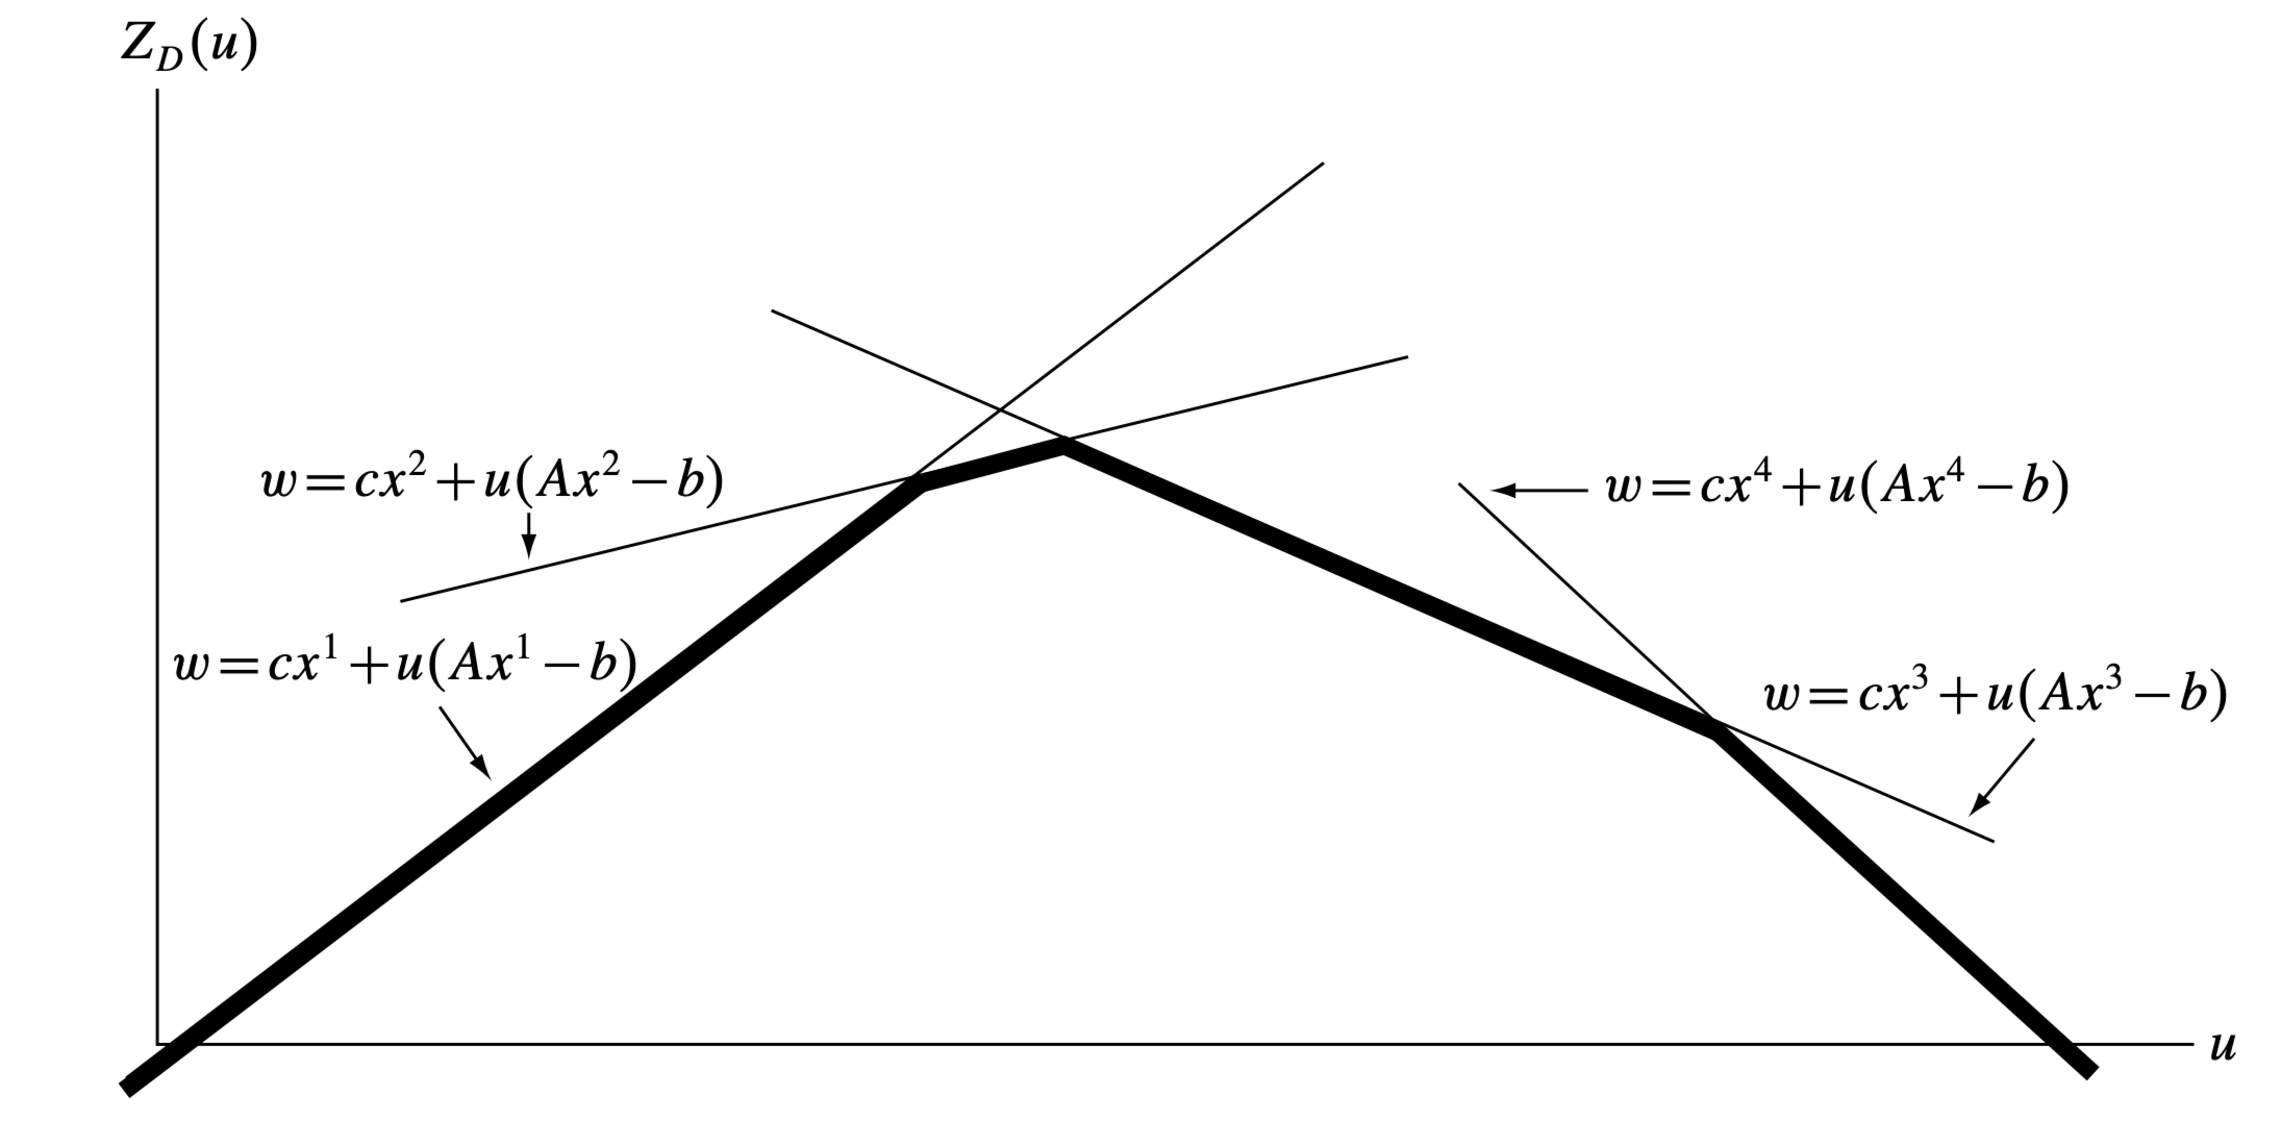
\includegraphics[width=0.9\textwidth]{figures/lag.pdf}
  \caption{$Z_D(u)$随$u$的变化(图中加粗黑线)\cite{Fisher2004} \\Fig~\ref{fig:lag}~ The value of $Z_D(u)$ as a function of $u$ \cite{Fisher2004}}
  \label{fig:lag}
\end{figure}

给定$u$的初始值$u_0$,后续乘子第$k$次迭代的值为$u^k$,迭代公式如下:
\begin{equation}
u^{k+1} = u^{k} + t_k(Ax^k-b) \label{eq:updlagmul}
\end{equation}

其中,其中$x^k$是$\mathrm{LR_{u^k}}$的最优解,
$t_k$是一个正数,称为迭代步长。
括号内的项$Ax^k-b$称作迭代方向。
Geoffrion\cite{Geoffrion1974}证明了当$t_k \rightarrow 0$
且$\sum_{i=0}^kt_i  \rightarrow \infty$时,$Z_D(u^k)  \rightarrow Z_D$。
常用的迭代步长公式如下:
\begin{equation}
   t_k = \frac{\alpha_k(Z^*-Z_D(u^k))} {||Ax^k-b||^2} 
\end{equation}

其中,$\alpha_k$是一个$(0,2]$之间的标量,$Z^*$是$Z_D$的上界,
通常由启发式获得。
$\alpha_k$的初始值一般设置为2,
当一定迭代次数后,$Z_D(u)$的值仍不能得到提升,则$\alpha_k$的值减半。

采用上述的次梯度法,不断迭代$u^k$的值,然后求解$Z_D(u^k)$,
使得松弛问题的目标函数值不断接近原问题的最优值。
需注意,由于松弛了P问题的约束,因此$Z_D(u^k)$的解对于P问题来说往往是不可行的。
通常采用启发式算法对$Z_D(u^k)$的解的进行修正,以获得P问题的可行解。

至此,本节推导了LR算法的原理。
第\ref{sec:LR框架}节将根据该原理,
为考虑节点失效风险的物流网络选址模型设计LR-ILS算法框架。

\section{算法设计}
\label{sec:LR框架}
本节将介绍采用LR-ILS算法求解考虑节点失效风险的物流网络选址模型的框架,
根据\ref{sec:LR概述}节所述,
LR算法主要包括获取下界(求解松弛模型)、获取上界、更新乘子等步骤。
注意,第\ref{sec:线性化}节中针对原模型进行了线性化处理,
所有推导内容均基于模型的线性化版本。
本节的LR-ILS算法框架参考了Snyder\cite{Snyder2005},
Yun等人\cite{yun2015, YUN2020}的文章,
以及Daskin\cite{Daskin书}使用LR关于求解UFL的方法。

为了便于理解,图\ref{fig:lr_frame}直观展示了LR-ILS的迭代流程,
图\ref{fig:lr_pseudo}提供了实现该算法的伪代码。
如图\ref{fig:lr_pseudo}所示,
在设计-ILS算法之前,需要先构造原问题M的松弛问题RM,
第\ref{subsec:约束松弛}节介绍了如何松弛问题M得到RM以及选取约束进行松弛的方法。
初始化已知最佳上界$ub^*$为正无穷,
最佳选址方案$Y^*$为空,
乘子初始化方法见第\ref{subsec:乘子更新}节。
LR-ILS算法迭代优化,
每次迭代使用精确方法获得下界(第\ref{subsec:下界获取}节),
根据下界解的选址方案构造启发式以获取上界可行解$ub$(第\ref{subsec:上界获取}节),
当上界解$ub$优于$ub^*$时,
则更新$ub^*$。
每次迭代中,LR-ILS算法使用次梯度法更新乘子,
第\ref{subsec:乘子更新}节介绍了乘子更新的方法。
当ILS条件被触发时,
ILS算法对当前解进行改进(第\ref{subsec:上界改进}节)。
若算法满足第\ref{subsec:停止条件}节的任意条件之一时,则退出迭代。
% 插入伪代码PDF代码
\begin{figure}[!ht] % use float package if you want it here
\setlength{\belowcaptionskip}{-0.5cm} 
  \centering
  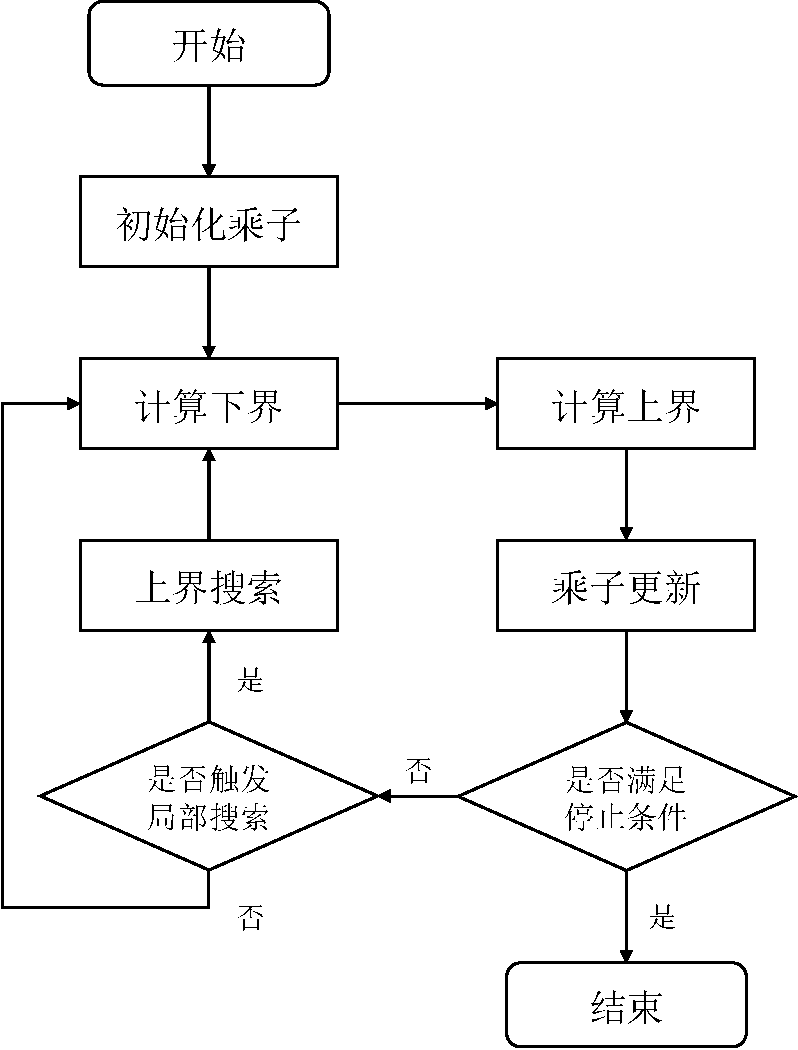
\includegraphics[width=0.5\textwidth]{figures/lr_frame.pdf}
  \caption{LR-ILS流程图\\Fig~\ref{fig:lr_frame}~ Flow chart for LR-ILS}
  \label{fig:lr_frame}
  \vspace{2ex}
\end{figure}

\begin{figure}[!ht]
    \centering
    \setlength{\belowcaptionskip}{-0.5cm} 
    \fbox{   
        \small
        \parbox[c]{0.8\textwidth}{
            \begin{algorithmic}[1] %每行显示行号
                \kaishu
                \Require 原模型M, 松弛模型RM  \Comment{ 参见第\ref{subsec:约束松弛}节}
                \State $\mu$ := 初始化乘子()  \Comment{ 参见第\ref{subsec:乘子更新}节}
                \State $ub^*$ := $+\infty$  
                \State $Y^*$ := $\emptyset$ 
                \Repeat
                    \State 下界$lb$, 选址方案$Y$ := 下界算法(RM($\mu$)) \Comment{参见第\ref{subsec:下界获取}节}
                    \State 上界$ub$ := 上界算法(M($Y$)) \Comment{ 参见第\ref{subsec:上界获取}节}
                    \If {$ub < ub^*$}                        %条件语句
                        \State $ub^*$ := $ub$
                        \State $Y^*$ := $Y$
                    \EndIf
                    
                    \State $\mu$ := 更新乘子($\mu$, $lb$, $ub^*$) \Comment{ 参见第\ref{subsec:乘子更新}节}
                    \If {ILS条件触发}                        %条件语句
                        \State $ub^*$ := ILS($ub^*$) \Comment{ 参见第\ref{subsec:上界改进}节}
                    \EndIf
                \Until{满足终止条件} \Comment{ 参见第\ref{subsec:停止条件}节}
                
                \State \textbf{return} $ub^*, Y^*$
            \end{algorithmic}
        }
    }
\caption{LR-ILS算法伪代码\\
    Fig~\ref{fig:lr_pseudo}~ Pseudocode for LR-ILS}
\label{fig:lr_pseudo}
\end{figure}



\subsection{约束松弛}
\label{subsec:约束松弛}
一般情况下,松弛不同的约束产生的效果不同,选取特定的约束进行松弛可加速求解过程。
Fisher\cite{Fisher2004}提出了两个选取松弛约束的准则:下(上)界的质量以及获得下(上)界所需计算量。
这两个准则是相互矛盾的,获得更高质量的界需要更多的计算量,较少的计算量生成的解的质量不佳。
因此,不同学者使用拉格朗日松弛求解选址问题时,构造松弛问题的方法也不尽相同,以权衡求解时长与求解质量。
Daskin\cite{Daskin书}使用拉格朗日求解UFL问题中松弛了关于所有客户都必须由某一个设施服务的约束,对应本文的约束(\ref{eq:st_assign2open})。
Snyder等人\cite{Snyder2005}求解RUFL问题松弛了每个客户的每一级都需要指派一个备用设施的约束,对应本文的约束(\ref{eq:st_trytimes})。
Yun等人\cite{YUN2020}松弛了已建成的设施才能成为客户的某一级的实体设施的约束,对应本文的约束(\ref{eq:st_assign2open})。

本文采用了Yun等人\cite{YUN2020}的松弛方法,松弛约束(\ref{eq:st_assign2open})。
使用该方法获得的松弛问题具有可继续拆分的特殊结构,利用此特性可以加快获取下界的过程。
第\ref{subsec:下界获取}节介绍了松弛问题的可拆分的特性以及获取下界的方法。

\subsection{下界获取}
\label{subsec:下界获取}
令原始模型为M,
设拉格朗日乘子$\mu = \{ \mu_{ij}\ge 0 | \forall i \in I , j \in J\}$,并将松弛的约束(\ref{eq:st_assign2open})与乘子相乘后与目标函数(\ref{eq:l_obj_model})相加,得到拉格朗日对偶问题的目标函数:
\begin{equation}
\begin{split}
\max_{\mu}\min_{x,y,w} C_D &= \sum_{j\in J}f_jy_j \\
&+ \sum_{i\in I}\lambda_i \sum_{k\in J_{ij}^+}\sum_{j\in \bar{J}} c_{kj} w_{ikj} \\
&+\sum_{i\in I}\sum_{j\in J}\mu_{ij}\left(\sum_{k\in J_{ij}^+}x_{ikj} -y_j \right)  
\end{split}
\end{equation}
整理可得,
\begin{equation}
\begin{split}
  \max_{\mu}\min_{x,y,w} C_D &= \sum_{j\in J} (f_j - \sum_{i\in I} \mu_{ij}) y_j \\
&+ \sum_{i\in I} \sum_{j\in J} \sum_{k\in J_{ij}^+} (\lambda_i c_{kj} w_{ikj} + \mu_{ij} x_{ikj}) \\
&+ \sum_{i\in I} \sum_{k\in J_{ij_0}^+}\lambda_i c_{kj_0} w_{ikj_0}  
\end{split}
\label{lag_obj}
\end{equation}
固定一组$\mu$的值,得到的松弛模型RM($\mu$)如下,为了方便阅读,本节给出了RM($\mu$)的约束,
这些约束与第\ref{sec:线性化}节中的线性约束是一致的。
\begin{equation}
\begin{split}
\min_{x,y,w} C_D(\mu) &= \sum_{j\in J} (f_j - \sum_{i\in I} \mu_{ij}) y_j \\
&+ \sum_{i\in I} \sum_{j\in J} \sum_{k\in J_{ij}^+} (\lambda_i c_{kj} w_{ikj} + \mu_{ij} x_{ikj}) 
+ \sum_{i\in I} \sum_{k\in J_{ij_0}^+}\lambda_i c_{kj_0} w_{ikj_0}  
\end{split}
\label{eq:rm_obj}
\end{equation}
\textit{s.t.}
\begin{gather}
\sum_{j\in J_{ii}^-}x_{iij} = \sum_{j\in J_{i{j_{0}}}^+} x_{ijj_0} = 1, \forall i \in I  \label{eq:rm_flow}\\
\sum_{k\in J_{ij}^-} x_{ijk} = \sum_{k\in J_{ij}^+} x_{ikj}, \forall i \in I, j \in J    \\
p_{iij} = x_{iij}, \forall i\in I, j\in J_{ii}^- \\
q_j\sum_{k\in J_{ij}^+} w_{ikj}= p_{ijj'}, \forall i \in I, j \in J, j'\in J_{ij}^- \\
\sum_{j\in J\cup\{i\}} \sum_{k\in J_{ij}^-} x_{ijk} \le R, \forall i\in I \\
w_{ijk} \le p_{ijk}, \forall i \in I, j \in J, j'\in J_{ij}^- \\
w_{ijk} \le x_{ijk}, \forall i \in I, j \in J, j'\in J_{ij}^- \\
w_{ijk} \ge p_{ijk} + x_{ijk} - 1, \forall i \in I, j \in J \cup \{i\}, j'\in J_{ij}^-
\end{gather}
\begin{equation}
0 \le w_{ijj'r} \le 1, \forall i \in I, j \in J, j'\in J_{ij}^- 
\end{equation}
\begin{equation}
x_{ijk} \in \{0,1\}, \forall i \in I, j \in J\cup \{i\}, k\in J_{ij}^-
\end{equation}
\begin{equation}
0 \le p_{ijk} \le 1, \forall i \in I, j \in J\cup \{i\}, k\in J_{ij}^- \label{eq:rm_p}
\end{equation}
\begin{equation}
y_{j} \in\{0,1\}, \forall j \in {J} \label{eq:rm_y}
\end{equation}

对于给定的任意$\mu$的值,RM($\mu$)的最优解一定是M的下界,相关证明见\ref{sec:LR概述}节。
根据目标函数(\ref{eq:rm_obj})的结构,松弛模型RM($\mu$)可拆分成两组子模型RM($\mu$)$_{sub1}$和RM($\mu$)$_{sub2}$。
其中,RM($\mu$)$_{sub1}$如下,
\begin{equation}
\min_{y} \sum_{j\in J} (f_j  - \sum_{i\in I}\mu_{ij}) y_j
\end{equation}
\textit{s.t.}
\begin{center}
   约束(\ref{eq:rm_y})
\end{center}
RM($\mu$)$_{sub2}$如下,
\begin{equation}
\max_{\mu}\min_{x,w} 
\sum_{i\in I} \sum_{j\in J} \sum_{k\in J_{ij}^+} (\lambda_i c_{kj} w_{ikj} + \mu_{ij} x_{ikj}) 
+ \sum_{i\in I} \sum_{k\in J_{ij_0}^+}\lambda_i c_{kj_0} w_{ikj_0}
\label{eq:rm2_obj}
\end{equation}
\textit{s.t.}
\begin{center}
   约束(\ref{eq:rm_flow}) - 约束(\ref{eq:rm_p})
\end{center}

在给定任意一组$\mu$的值的情况下,RM($\mu$)$_{sub1}$将变得十分容易求解,即给定一个最小化问题$\min_{y} \sum_{j\in J} (f_j  - \sum_{i\in I}\mu_{ij}) y_j$,其中$y_j,\forall j \in J$是0-1变量。
显然,
当$f_j - \sum_{i\in I}\mu_{ij} \ge 0 $时,$y_j=0$;
当$f_j - \sum_{i\in I}\mu_{ij} < 0 $时,$y_j=1$。

在给定任意一组$\mu$的值的情况下,RM($\mu$)$_{sub2}$还可进一步拆分成$|I|$个独立模型,
每个子模型RM($\mu$)$_{sub2}^i, \forall i \in I$是试错序列问题更一般的形式,
该问题的具体表述见第\ref{subsec:subprob}节。
RM($\mu$)$_{sub2}^i$与第\ref{subsec:subprob}节中介绍的问题的不同之处在于RM($\mu$)$_{sub2}^i$的目标函数不仅计算了期望成本,还计算了关于$\mu$的项。
不妨将$\mu_{ij}, \forall i \in I , j \in J$看作是客户$i$访问节点$j$的固定访问成本,
那么,RM($\mu$)$_{sub2}^i$可理解为从$i$点出发,
寻找一条到$j_0$的期望成本与固定访问成本最小的路径,
并且该路径经过的虚拟节点和实体节点总数不得大于$R$个。

本节已经给出了RM($\mu$)$_{sub2}$的线性混合整数规划模型,
使用上述的拆分方法固定$i\in I$的值即可获得RM($\mu$)$_{sub2}^i$,
然后可使用求解器求解RM($\mu$)$_{sub2}^i$。
当$\mu=0$时,
RM($\mu$)$_{sub2}^i$等价于第\ref{subsec:subprob}节中介绍的试错序列问题。
RM($\mu$)$_{sub2}^i$实质上是一个广义的最短路问题,
由于该问题是NP-hard问题,使用精确求解方法的计算时间较长,
而LR算法会多次迭代并反复调用求解该问题的方法,
因此本节给出两种快速求解RM($\mu$)$_{sub2}^i$的启发式算法以及一个精确方法。
启发式方法生成一个近似解,
精确方法在这个近似解的基础上进行改进,
可加快求解速度并获取下界的精确值。

(1){\textbf{插入启发式}}

已知客户$i$一定会从点$i$出发最终前往虚拟节点$j_0$,
因此可初始化一个从客户$i$到虚拟设施$j_0$的初始序列$s_i$。
在该方法中,$s_i$的期望成本与固定访问成本之和,即目标函数(\ref{eq:rm2_obj}),
记作$C_{lb}(s_i)$。
定义$s_i$中连续两点之间的位置集合为$P(s_i)$。
插入启发式算法的步骤如下:
\begin{enumerate}[leftmargin=0pt,itemindent=3.5\ccwd,nosep]
  \item[Step 0] 初始化序列$s_i:=[i,j_0]$, 计算$C_{lb}(s_i)$。
  \item[Step 1] 向$s_i$中每个位置$\rho \in P(s_i)$添加节点$j \in J$,并计算成本$C_{lb}^{\rho j}(s_i)$。
  \item[Step 2] 计算$\Delta_{\rho j} = C_{lb}(s_i) - C_{lb}^{\rho j}(s_i)$。
  \item[Step 3] 若所有$\Delta_{\rho j}<0$,则结束;否则将$\Delta_{\rho j}$最大值对应的节点$j^*$插入$s_i$的$p^*$位置,
  更新$s_i$,$P(s_i)$,$C_{lb}(s_i)$以及令$J:=J\backslash\{j^*\}$。
  \item[Step 4] 若$J=\emptyset$或$|s_i|=R+1$,则结束,否则重复Step 1-4。
\end{enumerate}

插入启发式从一个仅包含客户和虚拟节点的完整的初始序列出发,
因此初始序列的总成本等于惩罚成本。
每次插入实体节点之前,
评估每个节点插入每个位置之后得到的结果,
然后将实体节点插入序列中当前阶段的最佳位置,
使得总成本快速下降,直至不能插入任何节点。

(2){\textbf{构造启发式}}

已知客户$i$一定会从点$i$出发前往虚拟节点$j_0$。
构造启发式仅考虑每一阶段的最优,
向序列末尾逐个增加节点,
具体步骤如下:
\begin{enumerate}[leftmargin=0pt,itemindent=3.5\ccwd,nosep]
  \item[Step 0] 初始化序列$s_i:=[i]$, 令$C_{lb}(s_i)=0$。
  \item[Step 1] 计算所有点$j \in \bar{J}$添加至$s_i$末尾的增量成本$\Delta_{j} = C_{lb}(s_i+\{j\}) - C_{lb}(s_i)$。
  \item[Step 2] 令$j^* = \arg \min \Delta_{j}$,更新$s_i:=[s_i, j^*]$和$C_{lb}(s_i)$,$J:=J\backslash\{j^*\}$。
  \item[Step 3] 若$j^*=j_0$,则结束;若$|s_i|=R$,则$s_i:=[s_i, j_0]$,计算$C_{lb}(s_i)$并结束,否则重复Step 1-3。
\end{enumerate}

构造启发式从一个仅含客户的不完整路径出发,
每次向路径的末尾增加一个节点。
每次增加的过程都将增量成本最小的客户放在末尾,
直至添加了虚拟节点(构成了完整路径)或不再能添加节点(此时在末尾补充一个虚拟节点构成一个完整路径)。

上述两种算法均基于贪心算法,
插入启发式算法先接受高昂成本,
再插入节点以降低总成本。
插入启发式类似节约算法,初始成本很高,成本随节点插入逐渐降低。
构造启发式算法从无到有,逐渐拓展路径的长度,
每次拓展将增量成本最低的节点加入路径末尾。
插入启发式算法时间复杂度等于$O(m^2n)$,
构造启发式算法时间复杂度等于$O(mn)$,
其中$m=R$是客户拥有实体节点个数的上限,
$n=|J|$是备选点的数量。

需要注意,在给定$\mu$的值的前提下,上述的两种方法仅可以在多项式时间内获得近似最优解,
而不一定可以获得最优解。
这将导致RM($\mu$)$_{sub2}$不能获得最优解。
已知只有在子问题获得最优的前提下,才能保证下界小于上界(证明见第\ref{sec:LR概述}节)。
因此,采用上述方法获得的下界很有可能在最终收敛时超过上界,使算法无法证明上界的质量。

求解最短路问题经典的精确算法包括标签算法\cite{label}、脉冲算法\cite{pulse}等。
但这些算法不能直接应用于试错序列问题,
因为这些算法解决的问题中每个点并不存在失效概率,
且总成本等于路径长度简单和。
由于上述的启发式算法可以获得一个近似最优解,
本文将上述启发式算法获得的近似最优解带入深度优先搜索算法(Deep First Search, DFS),
并设计剪枝策略以求解试错序列问题的最优解。

(3){\textbf{DFS算法}}

DFS算法的伪代码如图\ref{fig:dfs_pseudo}所示。
DFS类似于构造启发式,
从客户点出发,
每一次向下分支就将一个节点添加至路径末尾,
直至遍历完这个分支的所有可能,
再选择该分支的某个分支继续遍历,
如此递归直至遍历完问题的所有可能。
对于该问题来说,递归的最大深度是有限的,
判定某个路径$s_i$是否到达最大深度的准则有三个: 
(1) $\bar{J} = \emptyset$; 
(2) $|s_i| = R$, 此时$s_i$只能以$j_0$结尾;
(3) $s_i$的已经以$j_0$结尾。
当搜索满足上述三种情况之一时,不再继续分支(到达叶子节点)。
然后计算路径成本$C_{ib}({s_i})$。
当$C_{ib}({s_i})$小于已知最优成本$C_{ib}({s_i^*})$,
则更新已知最优路径和已知最优成本。
DFS分支的过程采用了递归调用,
当搜索未达到最大搜索深度时,
继续向下分支的过程中,保存当前的父节点并在遍历完子节点及所有分支后恢复。
分支过程中,若当前路径的成本$C_{ib}({s_i+\{j\}})$大于已知最优成本$C_{ib}({s_i^*})$时,
则不再继续分支(剪枝)。

% \begin{figure}[hbt] % use float package if you want it here
%   %\setlength{\abovecaptionskip}{-0.2cm} %调整图片caption与正文之间的间距,table同理。可自己调整。
%   \setlength{\belowcaptionskip}{-0.5cm} 
%     \centering
%     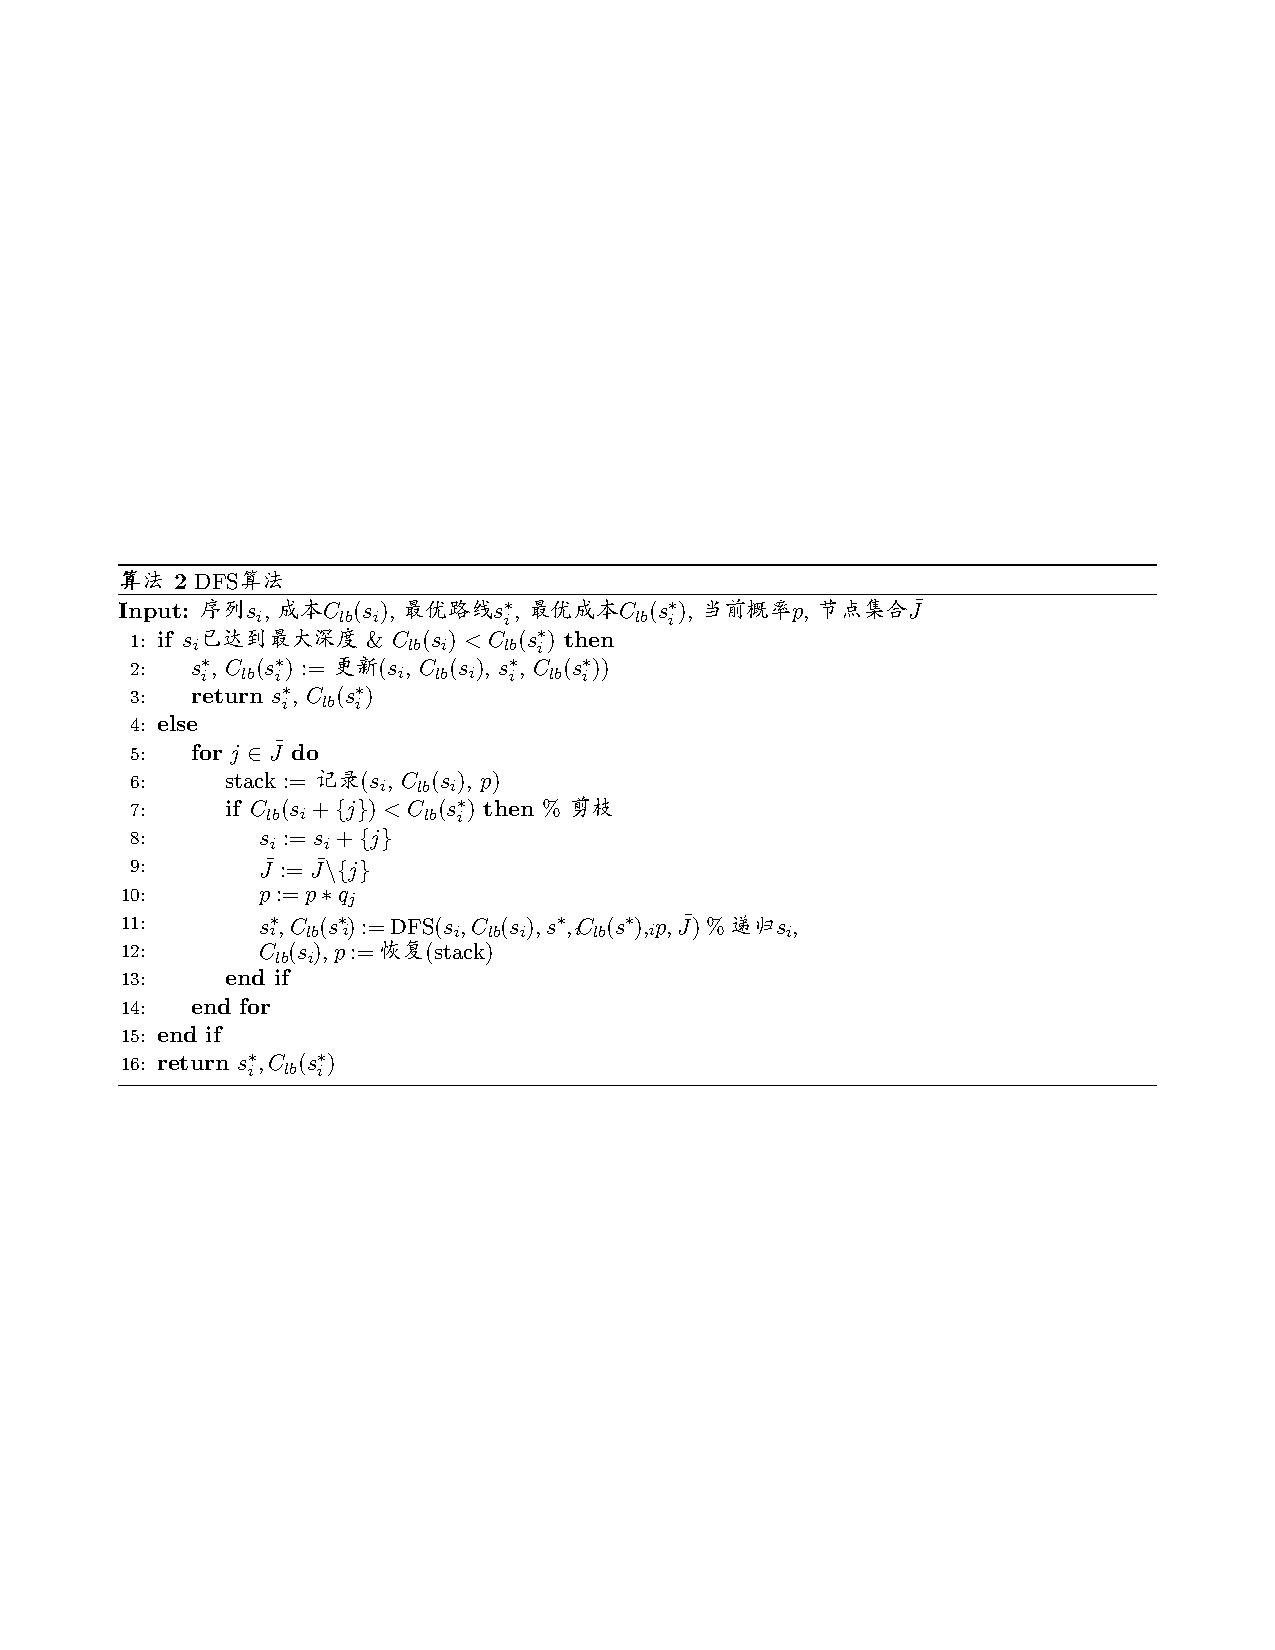
\includegraphics[width=\textwidth]{figures/dfs.pdf}
%     \caption{DFS算法伪代码。\\Fig~\ref{fig:dfs_pseudo}~ Pseudocode for DFS.}
%     \label{fig:dfs_pseudo}
% \end{figure}

\begin{figure}[htb]
    \centering
    \setlength{\belowcaptionskip}{-0.5cm} 
    \fbox{   
        \small
        \parbox[c]{0.9\textwidth}{
             \begin{algorithmic}[1] %每行显示行号
             \kaishu
                \Require 序列$s_i$, 成本$C_{lb}(s_i)$, 最优路线$s_i^*$, 最优成本$C_{lb}(s_i^*)$, 当前概率$p$, 节点集合$\bar{J}$
                % \Ensure 最优上界$ub^*$
                \If {$s_i$已达到最大深度~\&~$C_{lb}(s_i)<C_{lb}(s_i^*)$}                       %条件语句
                    \State $s_i^*$, $C_{lb}(s_i^*)$ := 更新($s_i$, $C_{lb}(s_i)$, $s_i^*$, $C_{lb}(s_i^*)$)
                    \State \textbf{return} $s_i^*$, $C_{lb}(s_i^*)$
                \Else
                    \For {$j \in \bar{J}$} 
                        \State stack := 记录($s_i$, $C_{lb}(s_i)$, $p$)
                        \If {$C_{lb}(s_i + \{j\})<C_{lb}(s_i^*)$} \% 剪枝
                            \State $s_i:=s_i + \{j\}$
                            % \State $C_{lb}(s_i)$ :=$C_{lb}(s_i + \{j\})$
                            \State $\bar{J} :=\bar{J} \backslash \{j\}$
                            \State $p: = p * q_j$
                            \State $s_i^*$, $C_{lb}(s_i^*)$ := DFS($s_i$, $C_{lb}(s_i)$, $s_i^*$, $C_{lb}(s_i^*)$, $p$, $\bar{J}$) \quad \% 递归
                            \State $s_i$, $C_{lb}(s_i)$, $p$ := 恢复(stack)
                        \EndIf  
                    \EndFor
                \EndIf
                \State \textbf{return} $s_i^*, C_{lb}(s_i^*)$
            \end{algorithmic}
        }
    }
\caption{DFS算法伪代码\\Fig~\ref{fig:dfs_pseudo}~ Pseudocode for DFS}
    \label{fig:dfs_pseudo}
\end{figure}


理论上,DFS可以求解任何最短路问题,
但是该算法并不是多项式时间算法,因此并不能保证计算时长在合理范围内。
本文可以采用DFS算法是因为搜索深度和客户的最大试错次数$R$正相关,
计算时间随搜索深度指数级增长,
但通常$R$的值并不会很大,
这使得DFS方案可行。
其次,上述的两个启发式方法可以获得近似解,
利用这个近似解可以在搜索过程中剪枝,
避免遍历所有情况。
最后,所有的成本均为非负值,即所有弧的权重为非负值,
这使得一条不完整路径$s_i$(不一定以$j_0$结尾)的产生的成本$C_{lb}(s_i)$
一定小于等于$s_i$被节点$\{j\}$拓展的路径的成本$C_{lb}(s_i+\{j\})$,
即到达子节点产生的费用一定大于等于父节点的费用。

综上,求解下界问题相当于求解一个最短路问题,
由于该问题是NP-hard问题,
本小节给出了两种多项式时间的启发式算法以获得近似最优解,
以近似最优解为已知最优解,
使用了DFS算法进行剪枝搜索以获得下界最优解。
此外,本小节给出了求解下界的数学规划模型,
亦可使用求解器对下界进行求解。

\subsection{上界获取}
\label{subsec:上界获取}
子问题的RM($\mu$)$_{sub1}$的解给出了选址方案$J^*$,
令选址方案对应的选址决策变量$y_j=1,\forall j\in J^*$
以及选址方案以外的选址决策变量$y_j=0,\forall j\in J \wedge j\notin J^*$,
作为约束条件加入原模型M中,
使用精确算法求解该模型,即可获得原模型的上界。
上界值等于建设节点的固定成本再加上客户的期望运输成本之和。
在已知选址方案$J^*$的情况下,
建设节点的固定成本等于被选中的候选节点的固定成本$f_j$的简单和。
已知选址方案$J^*$,求解客户的期望运输成本之和,
完全等价于第\ref{subsec:subprob}节介绍的试错序列问题,
即令拉格朗日乘子等于0。

然而,客户试错序列问题是一个NP-hard问题(第\ref{subsec:subprob}节给出了证明),
求解该问题的启发式算法以及精确方法已在第\ref{subsec:下界获取}节中介绍。
相较于下界,求解上界的过程较为简单:
首先,下界问题中所有的候选节点都可以被使用,
而在求解上界的过程只能使用已经建成的节点,问题规模缩小。
其次,下界问题中所有节点的都存在固定成本(拉格朗日乘子),
而上界问题中不存在固定成本。

由于本文考虑的是无容量限制的问题,
因此在给定选址方案后,模型可拆分成$|I|$个子问题,
这些子问题的最优解之和等于上界最优解,
每个子问题等价于试错序列问题也等价于RM$(\mu)_{sub2}^i$,
因此上界完全可以使用第\ref{subsec:下界获取}节中介绍的算法,
但为了加速获得每个客户的试错序列、获得高质量上界,
本节介绍了一种Dijkstra的变种算法,可以在多项式时间内求解上界。
注意该算法仅能快获得一个近似最优解,
并仅在不考虑访问节点固定成本(求解上界无拉格朗日乘子)的情况下表现良好。
类似Dijkstra原始版本,采用永久标号法的步骤如下:

\begin{enumerate}[leftmargin=0pt,itemindent=3.5\ccwd,nosep]
  \item[Step 0] 初始化每个节点的权重为$\infty$,到达每个节点的概率$p_j$为1,每个点的状态为未标记,设置客户为起点,每个节点的追踪标记等于客户。
  \item[Step 1] 从起点出发,计算到达所有未标记节点所需的成本,如果到达当前未标记节点的所需费用小于节点的权重,则更新该节点的权重。
  \item[Step 2] 在所有未标记节点中,找到权重最小的节点,将其设为起点,更新其到达概率等于上一个节点的到达概率乘以上一个节点的失效概率,更新其追踪标记为上一个起点。
  \item[Step 3] 重复Step 1-2。若当前起点为$j_0$,则结束,返回当前点的权重。
  若逆向追踪得到的路径中节点和客户总数等于$R$,则在路径最后补充一个$j_0$,计算路径成本,结束并返回路径成本。
\end{enumerate}

该算法对经典Dijkstra算法进行了修改,
在原有算法的基础上引入了到达该节点的概率,
并添加了终止规则。
算法的时间复杂度等于$O(mn)$,
其中$m$是客户最大尝试次数,
$n$是节点的个数。
该算法可以求解上界近似最优解,也可以求解下界近似最优解。
但是,求解下界解时加入了节点的固定访问成本,增加问题的复杂性,
使得这种方法求解下界的效果不佳。
在求解上界的过程中,由于不存在固定访问成本(拉格朗日乘子),
算法迭代更新虚拟设施$j_0$的权重的次数提升,
而每次更新$j_0$后,经过逆向追踪都可以获得一条更优的完整路径。
因此,求解上界的Dijkstra的变种算法并不适用于下界求解。
此外,Yun\cite{YUN2020}等人设计了一种辅助图方法,
基于辅助图,开发了另一种求解客户试错序列问题Dijkstra的变种算法。

回到整个拉格朗日算法框架,
获得上界的前提是子问题RM($\mu$)$_{sub1}$的解给出了选址方案$J^*$,
基于已知的选址方案可以获得质量较好的上界\cite{Daskin书,yun2015}。
本小节介绍了获取上界的方法,
根据已知的选址方案,使用Dijkstra变种算法生成每个客户的试错序列。
然而该方法对于求解下界效果不佳,但可以用来求解上界的近似最优解。
此外,求解下界的DFS方法同样适用于求解上界客户试错序列问题中,
将Dijkstra变种算法得到的解传递给DFS算法,
可在此近似解的基础上得到最优解,
该方法的详细操作见本章第\ref{subsec:下界获取}节。

\subsection{乘子更新}
\label{subsec:乘子更新}
第\ref{sec:LR概述}节介绍了LR算法常采用次梯度法进行乘子更新。
本文的算法和大多数LR算法一样\cite{Daskin书,yun2015,Snyder2005},
其算法的效率很大程度依赖乘子$\mu$的初始值。
合理的乘子初始值可以减少算法的迭代步骤,进而提升效率。
本文乘子初始值设定参考了Lim\cite{lim}的方法,
令$\mu^k=\{\mu_{ij}^k \ge 0\}$表示算法第$k$迭代时的乘子$\mu$的取值,
$\mu^0$表示乘子的初始值,其计算公式如下:

\begin{equation}
    \mu_{ij}^0 = \frac{1}{|J|}(\lambda_i c_{ij} + f_j), \forall i \in I, j\in J
\end{equation}

在第\ref{sec:LR概述}节拉格朗日松弛概述中,
公式(\ref{eq:updlagmul})展示了一般问题中拉格朗日乘子更新的迭代方法。
针对原问题M,乘子更新方法如公式(\ref{eq:updatemulti})所示,
\begin{equation}
\mu^{k+1}_{ij} = \mu^{k}_{ij} + t_k(\sum_{k\in J_{ij}^+}x_{ikj} -y_j),\forall i\in I,j\in J
\label{eq:updatemulti}
\end{equation}

其中,$t_k$表示迭代步长,计算方式如下,
\begin{equation}
t_k = \frac{\alpha_k(ub_k^* - lb_K)} {\sum_{i\in I}\sum_{j\in J}\sum_{k\in J_{ij}^+}|x_{ikj} -y_j|}
\label{eq:steplen}
\end{equation}

公式(\ref{eq:steplen})中$ub_k^*$和$lb_K$分别表示第$k$次迭代的已知最佳的上界和下界,
迭代步长系数$\alpha_k$是一个常量,
当算法连续$\kappa_{lb}$次迭代都未能使下界提升时(一般在情况下,下界会在此时产生振荡),
$\alpha_k$将除以比例因子$\theta_{lr}$,以缓解振荡。
关于公式(\ref{eq:steplen})右侧分母项,
本文参考了Yun\cite{YUN2020}关于迭代步长的设计,
修改了经典拉格朗日算法迭代步长分母取平方操作,
改用绝对值,以获得更优的收敛性。

\subsection{停止条件}
\label{subsec:停止条件}
为了在有限的时间内获得高质量的上界,
证明上界的质量,避免程序无意义的迭代,
当LR-ILS算法满足下列条件其中之一时,算法停止迭代:

\begin{enumerate}[label=(\arabic*),leftmargin=0pt,itemindent=3.5\ccwd, nosep]
    \item 迭代次数$k$大于等于最大迭代次数$\eta_{lr}$;
    \item 算法优化时长到达时间上限$\tau_{lim}$;
    \item 上下界间隙(gap)$(ub_k-lb_K)/ub_k \le \xi$;
    \item 迭代步长系数$\alpha_k <= \alpha_{min}$。
\end{enumerate}

条件(1)限制了拉格朗日算法的迭代次数,
条件(2)限制程序的运行时长,
条件(3)表明期望接受的解的优劣程度,
条件(4)避免算法后期不能提升下界的无用迭代。

\subsection{上界改进}
\label{subsec:上界改进}
上述小节\ref{subsec:约束松弛}至小节\ref{subsec:停止条件}已详细阐述了LR-ILS算法的细节,
使用上述方法可以获得可接受的结果\cite{yun2015,Daskin书,Fisher2004}。
但上述算法仍有一些缺陷:
上界解的选址方案是由下界解提供的,
下界解在算法后期收敛过程中并不能提供足够优质的选址方案,
或者下界在后期产生振荡。
为了加速算法上下界的收敛,
本节介绍的迭代ILS算法\deleted[id=yrf]{(Iterated Local Search, ILS)}对当前最佳选址方案$J^*$进行改进。


ILS算法可以作为独立的一种元启发式算法求解考虑节点失效风险的物流网络选址模型,
即在ILS每次迭代中,ILS提供选址方案,
再根据第\ref{subsec:上界获取}节获取上界的方法评估方案质量,
不断迭代直至算法连续多次迭代都不能获得更优解时结束。
但在本文中,将ILS嵌入LR迭代框架中(见图\ref{fig:lr_pseudo}),
当ILS算法被触发,会对$J^*$进行邻域搜索,
并将搜索到的更优解返回给LR,
以减少上下界之间的间隙。

本文嵌入的ILS算法的框架设计参考了Lourenço\cite{ils}等人书中内容,
该算法的伪代码如图\ref{fig:ils}所示。
ILS算法是一种基于单个解的局部搜索算法,
给定一个初始选址方案$J^*$(已知最优解),
ILS使用邻域算子搜索其邻域,
根据一定准则接受邻域中某个邻域解,
然后从这个邻域解出发继续搜索,搜索其邻域,
如此往复,迭代进行。
在搜索过程中,如果发现某个解优于已知最优解,
则用这个解替换已知最优解,并提前结束返回该解。

\begin{figure}[ht] % use float package if you want it here
%\setlength{\abovecaptionskip}{-0.2cm} %调整图片caption与正文之间的间距,table同理。可自己调整。
\setlength{\belowcaptionskip}{-0.5cm} 
  \centering
  \fbox{   
        \small
        \parbox[c]{0.9\textwidth}{
            \begin{algorithmic}[1] %每行显示行号
                \kaishu
                \Require 选址方案$J^*$
                \State 已知最佳选址方案$J^*_{best}$ := $J^*$
                \Repeat 
                    \State 邻域$\mathcal{N}(J^*)$ := 邻域算子($J^*$)
                    \State $obj_{\mathcal{N}(J^*)}$ := 目标函数($\mathcal{N}(J^*)$)
                    \If {min($obj_{\mathcal{N}(J^*)}$)$< obj_{J^*_{best}}$}
                        \State $J^*_{best}$ := $j$
                        \State \Return $J^*_{best}$
                    \Else 
                        \State $J^*$ := 接受准则($\mathcal{N}(J^*)$)
                    \EndIf
        
                \Until 终止条件满足
                \State \Return $J^*_{best}$
            \end{algorithmic}
        }
    }
  \caption{ILS算法伪代码\\Fig~\ref{fig:ils}~ Psuedocode for ILS}
  \label{fig:ils}
\end{figure} 

算法的邻域搜索过程包括三种算子\cite{sa_lp,ts_lp}:关闭、开启、交换算子。
关闭算子是指关闭$J^*$中的某个已建设节点,使得固定成本下降,运输成本上升,
以在效益背反的博弈中使得总成本降低;
开启算子是指开启$J^*$中的某个未建设节点,使得固定成本上升,运输成本下降;
交换算子是指交换$J^*$中关闭某个已建设节点并开启某个未建设的节点。

每次迭代ILS评估所有邻域解的质量,发现更优的解将返回这个解,
若没有发现更优解,则接受一个相对较差的解。
接受准则借鉴了模拟退火算法的设计思路\cite{sa},
当邻域解$j^*\in \mathcal{N}(J^*) $未改进$J^*_{best}$时,
$j^*$仍有$e^{[{obj(j^*)-obj(J^*_{best})}] / T}$的概率被接受,
其中$T$为模拟退火温度,
其初始值设定为$T_0$。
$T_0$的取值应使得ILS在$obj(j^*)/obj(J^*_{best})=\theta_{sa}$时的接受概率等于50\%,
其中$\theta_{sa}$是常数。
即在ILS算法初次迭代时,如果某个邻域解的目标函数是已知最优目标函数值$\theta_{sa}$倍时,
ILS有50\%的概率接受这个解。
温度$T$随ILS迭代次数线性减少,但不低于$T_{min}$。

当LR迭代过程中,连续$\kappa_{ub}$次未降低上界时,
ILS算法被触发。
ILS算法至多迭代$\eta_{ils}$次,
该值应设置成一个较小的数,
因为过多的搜索次数将降低算法整体的迭代效率。
此外,ILS也可以将当前迭代的邻域传递给下一次ILS触发,
相当于搜索算法的重启操作\cite{vrpdst},
重启ILS很可能产生不同的搜索过程,进而提升发现更优解的概率。

% 此外,除了在迭代过程中可以使用ILS改进上界,
% 在LR-ILS算法结束后,将最佳选址方案转为约束条件,
% 添加至原模型M中,
% 并使用求解器求解一次模型,
% 可以获得更加优质的上界,
% 以解决第\ref{subsec:上界获取}节Dijkstra变种算法不能获得最优试错序列的缺点。

\section{本章小结}
\label{sec:小节4}
本章阐述了求解考虑节点失效风险的物流网络选址模型的算法,
第\ref{subsec:约束松弛}节松弛了模型中所有客户必须分配给已建设设施的约束,
使得松弛问题可以拆分成多个子问题。
其中求解每个子问题的过程等价于一个最短路问题,
第\ref{subsec:下界获取}节采用了启发式加深度优先搜索算法求解这个子问题。
松弛模型的节提供了选址方案,
将该选址方案提供给上界问题(原模型),
求解上界的过程仍然是求解最短路问题,
第\ref{subsec:上界获取}节开发了Dijkstra变种算法,
在多项式时间内求解客户在给定选址方案的情况下的试错序列。
第\ref{subsec:乘子更新}节和
第\ref{subsec:停止条件}节阐述了拉格朗日乘子更新和停止条件。
特别地,本章的第\ref{subsec:上界改进}节给出了上界改进的方法,
介绍了一种可以嵌入拉格朗日松弛迭代中可以改进上界的ILS算法。
最后,值得一提的是,本章中所有的求解上界或下界的过程,
都可以使用求解器进行求解,
虽然求解时间随问题规模指数增长,
但提供了一种检验自设计算法有效性的方法或标准。
第\ref{cha:算法性能章}章对算法的性能进行了详细的分析,包括求解时间、求解质量等指标。
                % 第四章
 \setlength{\baselineskip}{20pt}
 \interfootnotelinepenalty=10000
 \setlength{\tabcolsep}{5pt}
\chapter{数值实验设计及算法性能分析}
\label{cha:算法性能章}

% \tinytodo[inline]{修改章节导言}
\added[id=yrf]{本章将进行一系列实验以测试LR-ILS算法的性能,
以此验证算法的有效性,
特别关注于LR-ILS算法在解决大规模问题时的求解质量和求解时长。}
第\ref{sec:实验设计}节阐述了计算实验的平台与环境,
算法的参数取值以及数据来源等。
% % 第\ref{sec:数值实验}节详细分析了数值实验的结果,
% % 特别是对算法的性能进行了分析。
% 本节进行数值实验的
% 目的是分析算法求解大规模问题的能力,
% 以判断其求解现实问题的实用性。
第\ref{sec:综合性能}节对算法的整体性能进行了分析;
第\ref{sec:下界性能}节和第\ref{sec:上界性能}节分别分析了算法求解上下界的能力;
第\ref{sec:乘子性能}节讨论了不同拉格朗日乘子初始设置和更新策略的效果;
第\ref{sec:线性化优势}节讨论了模型线性化带来的求解增益效果;
第\ref{sec:算例结果}节展示了算例的选址结果及灵敏度分析结果;
最后,第\ref{sec:本章小结5}节总结了本章的主要工作。

\section{实验设计}
\label{sec:实验设计}
实验采用的计算平台的配置如下:
主频3.1Ghz的6核心12线程CPU(AMD 1600)搭配8Gb内存,
操作系统为Windows 10。
LR-ILS算法主程序由Matlab 2022b构建,
使用Python 3.9调用Gurobi 9.5.2进行建模。
为了加快程序运行速度,
额外使用了Matlab Coder将算法的关键步骤编译成二进制mex文件,
并在其中使用了多线程计算。

本文的第\ref{cha:LR算法}章LR-ILS算法设计考虑了一系列控制算法效果的参数,
经过多次的预实验,这些参数的取值如表\ref{table:参数取值}所示。
在预实验中,给定算法的参数初始值(根据经验预估),
每次调整固定算法的其他参数值,只调整一个参数,
直至在该参数下算法效果最好,
再更换其他参数进行调整。
\vspace{-2ex}
\begin{table}[!htb]\normalsize   %%\small是为了设置表格中的字体比正文小
\setlength{\abovecaptionskip}{1ex} 

\centering
\renewcommand\arraystretch{0.8}
\caption{LR-ILS算法参数取值\\Table~\ref{table:参数取值}~Parameter Setting for LR-ILS}
\small{
	\begin{tabular}{p{1.6cm}<{\centering} p{1.6cm}<{\centering} p{1.6cm}<{\centering} p{1.6cm}<{\centering} p{1.6cm}<{\centering} p{1.6cm}<{\centering} }
		% \begin{tabular}{c}{l}
		\toprule %[2pt]设置线宽  
		\multicolumn{2}{c}{LR} & \multicolumn{2}{c}{ILS} & \multicolumn{2}{c}{Gurobi}\\
		\cmidrule(r){1-2} \cmidrule(r){3-4} \cmidrule(r){5-6}
		参数   & 取值 & 参数  & 取值 & 参数  &  取值 \\
		\midrule %[2pt]
		$\alpha_0$      & 2      & $\theta_{sa}$  & 1.2    & MIPGap    & 0.00001\\
		$\alpha_{min}$  & 0.0001 & $T_{min}$      & 0.0001 & TimeLimit & 1000\\
		$\theta_{lr}$   & 1.05    & $\kappa_{ub}$  & 200\\
		$\kappa_{lb}$   & 10     & $\eta_{ils}$   & 10\\
		$\eta_{lr}$     & 3000  \\
		$\tau_{lim}$    & 1000(s)  \\
		$\xi$           & 0.01  \\
		\bottomrule %[2pt] 
	\end{tabular}
}
\vspace{-1ex}
\label{table:参数取值}
\end{table}

本节数值实验采用的数据来源于Snyder\cite{Snyder2005},
是选址研究的经典数据集。
该数据集包含了49、88、150个点的三套数据,
可在Snyder\cite{Snyder2005}的个人主页\footnote{https:\slash \slash coral.ise.lehigh.edu\slash larry\slash research\slash data-sets-for-reliability-models-for-facility-location-the-expected-failure-cost-case}下载。
原始数据为1990年美国房价普查数据,
包含了美国各个州的人口和房价数据。
学者们常使用该数据模拟节点选址中的固定成本和需求\cite{Daskin书,Snyder2005,yun2015,Cui2010}。
本文参考了Yun\cite{yun2017}的处理方法,
令客户的需求等于州人口数除以$10^5$,
节点的固定成本$f_j, \forall j \in J$等于房价的中位数,
令节点失效的概率等于$q_j = \rho e^{-f_j/200000},\forall j \in J$,
其中$\rho$是控制失效概率大小的参数,
惩罚成本$\pi = 10^4$, 客户最大尝试次数$R=5$。
此外,令客户点等于需求点,即$I=J$,
这样可以使图$G$中点的数量翻倍,
也不必再区分数据集中哪些点是客户点或是节点候选点。
令任意两点之间的距离等于大圆距离,
该距离的具体计算方法可见参考文献\cite{Snyder2005,Yongzhen,yun2015}。


\section{综合求解性能分析}
\label{sec:综合性能}

本节分析了算法的综合性能,
分为四个内容,
首先对比测试了LR-ILS算法求解不同规模、不同参数取值的数据的性能;
其次,对比Gurobi分析了求解时间和求解质量;
然后,分析了模型中两个重要参数$\rho$和$R$对LR-ILS求解性能的影响;
最后,通过上下界优化曲线直观展示了算法的迭代过程。
附录B展示了使用LR-ILS求解包含49、88、150个点的数据集的所有计算结果,
其中参数
$\rho$分别取0.01、0.05、0.1、0.2、0.3、0.4、0.5,
$R$分别取2至10。

\subsection{求解性能对比}
表\ref{table:LR与GRB}分别展示了LR-ILS算法和Gurobi求解器求解
49个点、88个点、150个点以及参数$\rho$不同取值的计算结果。
表\ref{table:LR与GRB}的所有实验均默认参数$R=5$,
其中gap值等于上下界之差除以上界,
相对差距等于LR-ILS得到的上界值减去Gurobi得到的上界值再除以二者之间的较小值,
因此相对差距为负时,LR-ILS获得了更优的上界,该值越小表明LR-ILS得到的结果越好。
相对速度等于Gurobi的求解时间除以LR-ILS的求解时间,
该值越大表明LR-ILS求解速度越快。

\begin{table}[hbt]
	\setlength{\abovecaptionskip}{-0.05cm} %调整图片caption与正文之间的间距,table同理。可自己调整。
	\setlength{\belowcaptionskip}{-0.2cm} 
	\centering
	\renewcommand\arraystretch{1}
	\caption{LR-ILS与Gurobi结果对比\\Table~\ref{table:LR与GRB}~Results for LR-ILS and Gurobi}
	\resizebox{\linewidth}{!}{
		\begin{tabular}{cccccccccc}
		\toprule %[2pt]设置线宽 
		\multirow{2}[0]{*}{数据集} & \multirow{2}[0]{*}{$\rho$} & \multicolumn{3}{c}{LR-ILS} & \multicolumn{3}{c}{Gurobi} 
		& \multirow{2}[0]{*}{\makecell[c]{相对\\差距(\%)}} & \multirow{2}[0]{*}{\makecell[c]{相对\\速度(倍)}} \\
		\cmidrule(r){3-5} \cmidrule(r){6-8}
		&       & 上界    & gap(\%) & 时间(s) & 上界    & gap(\%) & 时间(s) &       &  \\
		\midrule %[2pt]
		49    & 0.01  & 965061.90 & 0.99  & 0.21  & 965227.40 & 0.19  & 39.37 & -0.02 & 187.48 \\
		49    & 0.05  & 1018144.58 & 0.89  & 0.40  & 1021312.55 & 2.54  & 1000.00 & -0.31 & 2500.00 \\
		49    & 0.10  & 1076487.05 & 0.99  & 0.53  & 1077872.84 & 8.92  & 1000.00 & -0.13 & 1886.79 \\
		49    & 0.20  & 1198200.17 & 1.15  & 13.27 & 1224021.70 & 19.67 & 1000.00 & -2.16 & 75.36 \\
		88    & 0.01  & 1361557.62 & 1.00  & 0.76  & 1360245.50 & 1.16  & 1000.00 & 0.10  & 1315.79 \\
		88    & 0.05  & 1440083.62 & 0.99  & 1.18  & 1438341.99 & 6.09  & 1000.00 & 0.12  & 847.46 \\
		88    & 0.10  & 1527361.61 & 0.92  & 6.67  & 1544990.68 & 12.90 & 1000.00 & -1.15 & 149.93 \\
		88    & 0.20  & 1721135.80 & 2.70  & 98.52 & 1762412.99 & 23.85 & 1000.00 & -2.40 & 10.15 \\
		150   & 0.01  & 2176492.30 & 1.00  & 13.63 & -     & -     & 1000.00 & -     & - \\
		150   & 0.05  & 2279427.84 & 1.39  & 19.26 & -     & -     & 1000.00 & -     & - \\
		150   & 0.10  & 2391069.73 & 1.93  & 46.93 & -     & -     & 1000.00 & -     & - \\
		150   & 0.20  & 2611120.81 & 3.31  & 184.14 & -     & -     & 1000.00 & -    & - \\
		  \bottomrule %[2pt]   
	\end{tabular}%
	}
 \vspace{-2ex}
	\label{table:LR与GRB}
\end{table}%

数值结果表明
LR-ILS算法的显著优势在于能够在相对较短的时间内
获得质量较高的近似最优解,
具体分析如下:
首先,从求解的时间和速度进行分析,
除了第一组数据外,
Gurobi求解时长均到达了设置的最大运行时长,
并且150个点的问题全部没有在规定时间内得到结果。
相比之下,LR-ILS算法的求解时间显著优于Gurobi,
注意到该问题为NP-hard问题,
问题规模随节点数量增加而指数级增长。
因此在求解49个点的问题时,LR-ILS算法的求解效率是Gurobi的数千(百)倍,
求解88个点的问题时,求解效率退化至数百倍,
求解150个点的问题时,求解效率退化至数十倍,
表\ref{table:LR与GRB}中``相对速度(倍)''列展示了这种趋势。
相比Gurobi,
LR-ILS算法的求解速度具有显著优势。
在上界质量接近的情况下,
LR-ILS的求解时间更短。

其次,从求解的质量进行分析。
对比Gurobi,
对于49个点的全部算例,
LR-ILS获得了更加优质的上界;
对于88个点的部分算例,
LR-ILS的上界值略差于Gurobi,
但二者之间的相对差距($\le 0.12\%$)几乎可以忽略不计;
对于150个点的全部算例,
LR-ILS得到了上界的计算结果,
而Gurobi未能得到可行解。
Gurobi的上界质量和LR-ILS上界质量相差无几,
观察表中的gap值项,
除了第一组较为简单的数据集之外,
Gurobi的gap值均大于LR-ILS的gap值。
这表明证明上界的最优性方面,
Gurobi明显不如LR-ILS,
即拉格朗日松弛得到的下界优于Gurobi内置的线性松弛得到的下界。

\subsection{算例参数\texorpdfstring{$\rho$}{p}的影响}
尽管LR-ILS可以求解更复杂的问题并提供了优质下界,
但观察到无论是LR-ILS还是Gurobi,
求解问题所需的时长以及gap值都随参数取值的变化而变化。
% 为了探索参数对LR-ILS算法求解的影响,
% 本节的后续内容分析了在相等规模的情况下LR-ILS求解不同参数取值的算例性能,
% 以及讨论了产生这些现象的原因。
参数$\rho$的取值将影响LR-ILS算法的求解性能。
该参数控制节点的失效概率大小,
使得节点的失效概率接近$\rho$自身,
但由于节点的建设成本不一,
各个节点的失效概率也不相等。
随着参数$\rho$的增加,
模型的复杂程度提高,
LR-ILS算法的表现也越来越退化。
本节使用了49个点的算例进行测试,
$\rho$取0.1至0.9间隔为0.1的9个值,
$R$取2至10的整数,
求解时间及gap值随$\rho$变化
如图\ref{fig:result_time_rho}和图\ref{fig:result_gap_rho}所示。


\begin{figure}[ht] % use float package if you want it here
%\setlength{\abovecaptionskip}{-0.2cm} %调整图片caption与正文之间的间距,table同理。可自己调整。
\setlength{\belowcaptionskip}{-0.5cm} 
  \centering
  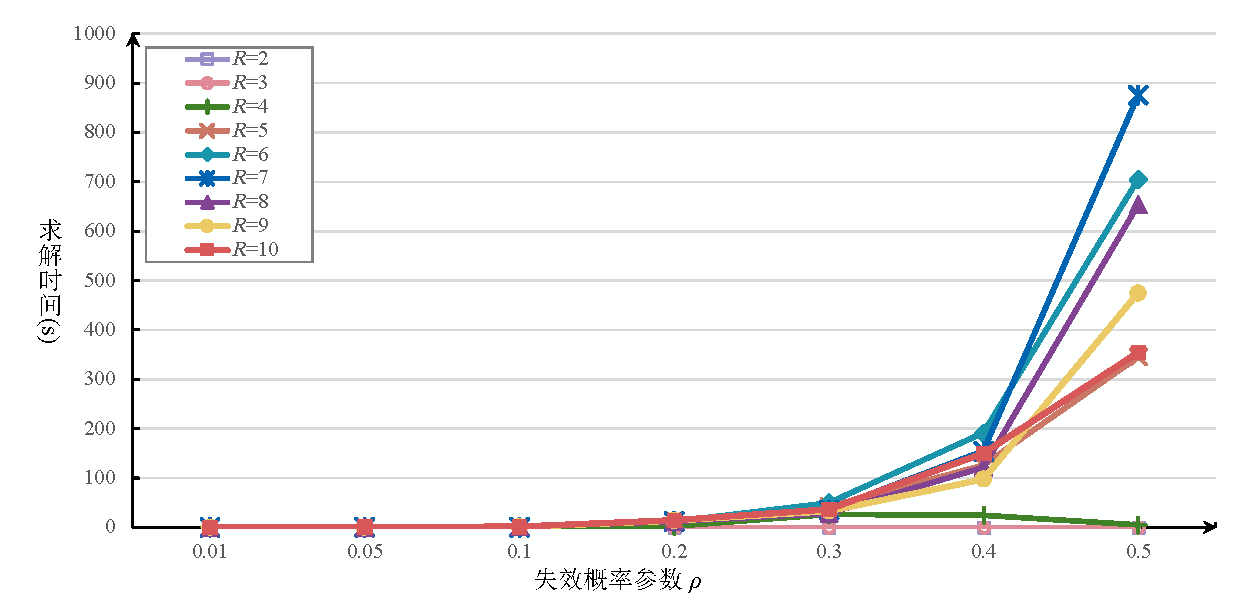
\includegraphics[width=0.9\textwidth]{figures/result_time_with_rho.pdf}
  \caption{LR-ILS算法求解时间随$\rho$的变化曲线\\Fig~\ref{fig:result_time_rho}~ Curves of LR computating time with respect to $\rho$}
  \label{fig:result_time_rho}
\end{figure}

\begin{figure}[ht] % use float package if you want it here
	%\setlength{\abovecaptionskip}{-0.2cm} %调整图片caption与正文之间的间距,table同理。可自己调整。
	\setlength{\belowcaptionskip}{-0.5cm} 
	  \centering
	  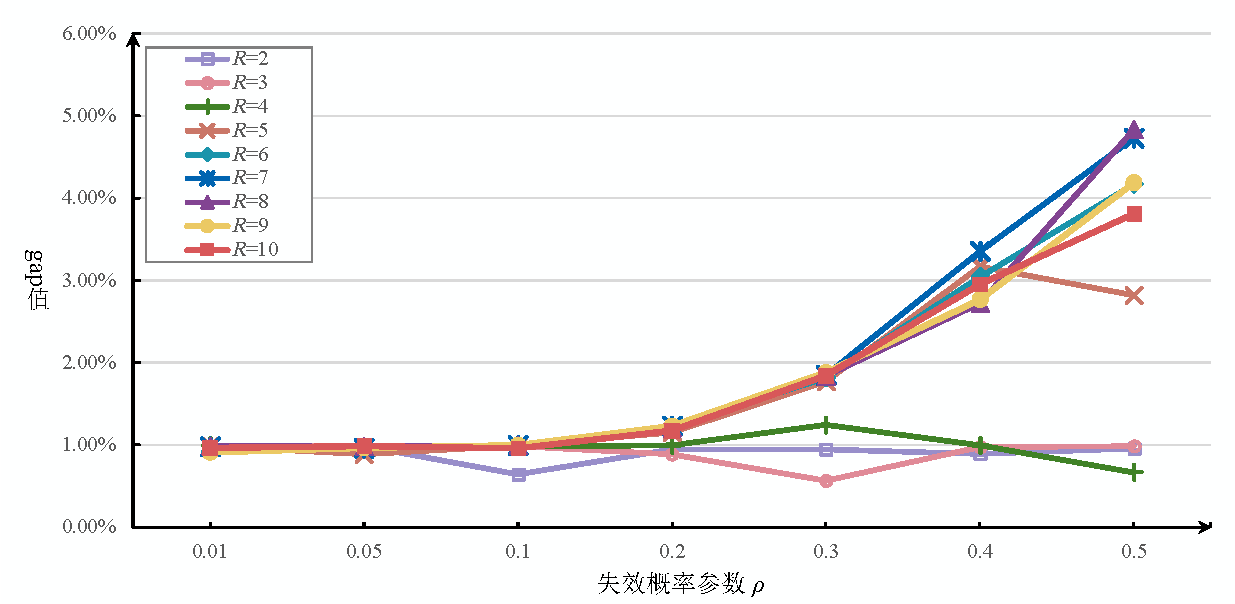
\includegraphics[width=0.9\textwidth]{figures/result_gap_with_rho.pdf}
	  \caption{LR-ILS算法求解gap随$\rho$的变化曲线\\Fig~\ref{fig:result_gap_rho}~ Curves of LR gap values with respect to $\rho$}
	  \label{fig:result_gap_rho}
\end{figure}


图\ref{fig:result_time_rho}和图\ref{fig:result_gap_rho}的横坐标轴表示参数$\rho$的变化范围,
纵坐标轴分别表示在此$\rho$取值下求解所需的计算时间以及结果的gap值,
不同颜色的线条表示不同$R$取值的结果。
首先分析求解时间与$\rho$的关系,
图\ref{fig:result_time_rho}中可见,参数$\rho$显著影响了求解的时间,
在大多数测试中,求解时间随参数$\rho$的增加而指数级增加,
特别是在$\rho=0.2$至0.5的区间内,
求解时间的增加变化十分明显。
这表明随着$\rho$取值变大,模型的复杂度提升,求解的难度随之增加。
求解难度提升的本质原因是随着节点失效概率增加,
求解客户试错序列的难度增加,
即安排客户不同等级的备用节点以充分降低惩罚成本,
以及在设施建设成本、期望运输成本以及惩罚成本三者之间权衡的难度增加。
这导致了算法的精确过程,例如DFS搜索过程的效率显著降低,
由于节点的失效概率增加,惩罚成本所占比重增加,
启发式不能提供一个优质的近似解导致DFS剪枝过程受影响,搜索次数、深度明显增加。
注意到在一些测试中,求解时长并不受$\rho$的显著影响,
这是因为这些测试的$R$的取值较小($\le 4$),
每个客户的常用节点和备用节点的指派任务较为简单(最优客户试错序列),
因此求解时长变化并不明显。
在$R \le 4$的情况下,
对于49个点的算例,LR-ILS算法可以在很短的时间内求解得到近似最优解。
对于$R$取值较大的情况,
LR-ILS也能在可接受的时间内求解得到一个结果。

其次,分析求解结果gap值随$\rho$的变化的关系。
与求解时间随$\rho$变化的情况类似,
在大部分测试中,
gap值同样随$\rho$增加而增加,
特别是在$\rho=0.2$至0.5的区间内的变化较为明显。
gap值证明了上界的最优性,
图\ref{fig:result_gap_rho}中所有的结果表明,
LR-ILS求解结果的gap值不超过5\%,
即LR-ILS算法求解49个客户点与49个备选点(或49个点以下)的问题时,
有能力得到一个在5\%误差内的近似最优解。
同样,$R \le 4$的测试结果中,
gap值受$\rho$变化的影响较小。
本文中LR-ILS算法设置停止准则的gap值为0.01,
因此一些测试的gap值只停留在1\%附近,
若改变算法参数,gap值有望进一步降低。

\subsection{算例参数\texorpdfstring{$R$}{R}的影响}
注意到在图\ref{fig:result_time_rho}和图\ref{fig:result_gap_rho}中,
并非$R$的值越大,求解的时间越久或gap值越高。
例如,在$\rho=0.5$时$R=7$的求解时间最长,
并且求解结果的gap值较高。
图\ref{fig:result_time_r}和图\ref{fig:result_gap_r}
从另一个角度分析了求解时间和gap值受参数$R$的影响程度。
图\ref{fig:result_time_r}和图\ref{fig:result_gap_r}
的横坐标表示$R$的不同取值,
纵坐标分别表示求解时间和gap值,
不同颜色的线条表示不同$\rho$的取值。

\begin{figure}[ht] % use float package if you want it here
	%\setlength{\abovecaptionskip}{-0.2cm} %调整图片caption与正文之间的间距,table同理。可自己调整。
	\setlength{\belowcaptionskip}{-0.5cm} 
	  \centering
	  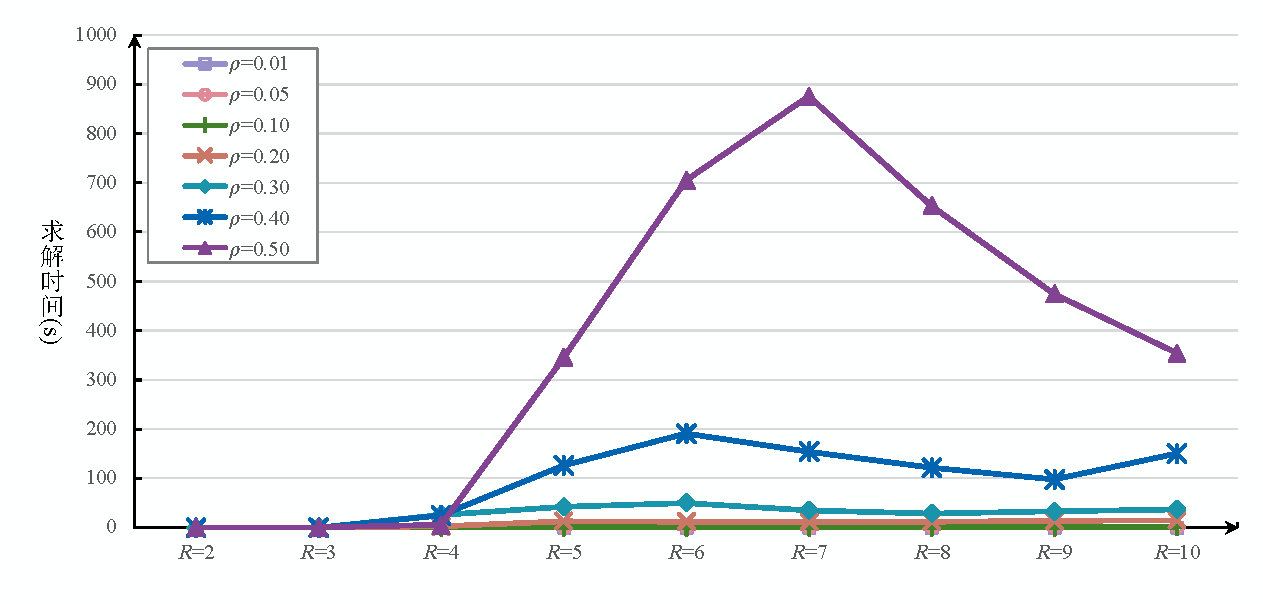
\includegraphics[width=0.9\textwidth]{figures/result_time_with_R.pdf}
	  \caption{LR-ILS算法求解时间随$R$的变化曲线\\Fig~\ref{fig:result_time_r}~ Curves of LR computating time with respect to $R$}
	  \label{fig:result_time_r}
\end{figure}
	
\begin{figure}[ht] % use float package if you want it here
	%\setlength{\abovecaptionskip}{-0.2cm} %调整图片caption与正文之间的间距,table同理。可自己调整。
	\setlength{\belowcaptionskip}{-0.5cm} 
		\centering
		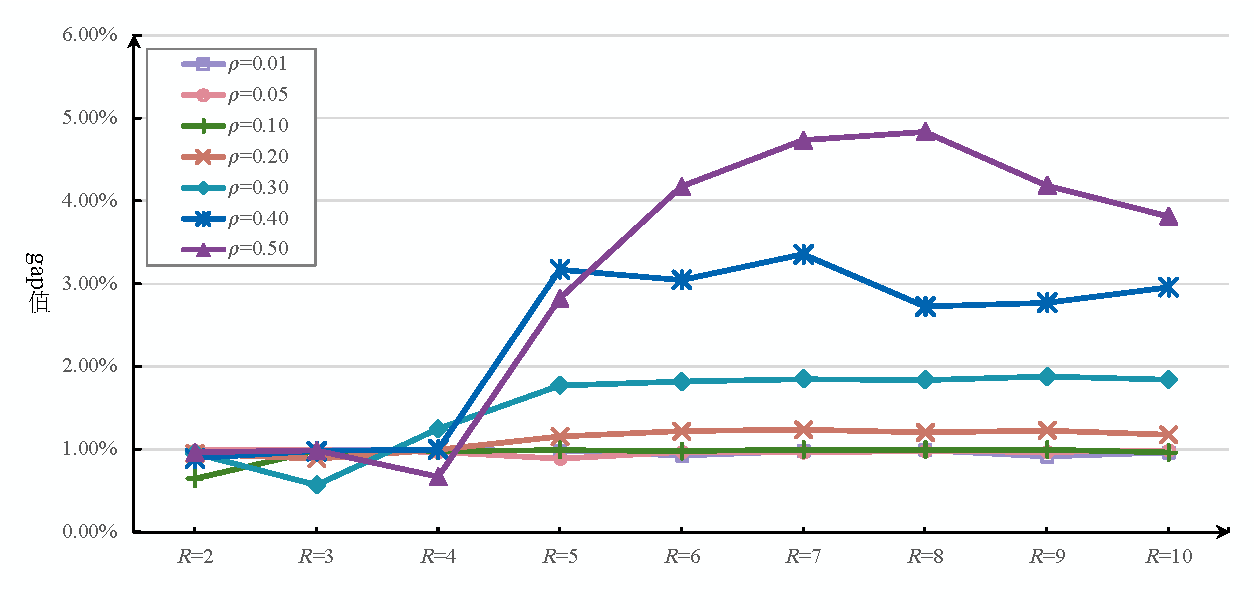
\includegraphics[width=0.9\textwidth]{figures/result_gap_with_R.pdf}
		\caption{LR-ILS算法求解gap随$R$的变化曲线\\Fig~\ref{fig:result_gap_r}~ Curves of LR gap values with respect to $R$}
		\label{fig:result_gap_r}
\end{figure}

在\ref{fig:result_time_r}和图\ref{fig:result_gap_r}中,
LR-ILS求解的时长以及gap值随参数$R$的增加
先上升后下降,这种趋势在$\rho$取值较大时更为明显。
产生该现象的原因是参数$R$和参数$\rho$对问题求解复杂程度的复合影响。
在$\rho$取值较大时,惩罚成本占比较高,
随着$R$不断增加,为了降低惩罚成本,
优化过程会为每个客户尽可能多地指派备用节点以降低惩罚成本,
因此求解模型的时间增加且gap值增加。
当$R$增加至一定值时,
求解时间或gap值增加到顶点。
对于49个点的算例来说,这个值是7或8。
随后,$R$值提升导致
客户前往接受惩罚的概率降低,
再增加$R$的值,
惩罚成本在总成本中的占比显著降低,
这反而降低了求解子问题的难度,
求解子问题时DFS剪枝策略又开始生效,
求解效率提升。
但是,随着$R$增加,问题更加复杂,
因此求解时间和gap值的表现也很难恢复至之前$R$取值较小的水平。

注意,上述分析单纯从数值角度出发,
在实际中,很少有节点伴随如此高的失效概率
($\rho = 0.5$时节点平均失效概率为35.14\%),
因此该算法仍可以求解现实问题。
本文同样给出了提高求解质量的途径:
参数调整方面,可适当增加LR的迭代次数,降低迭代步长比例因子,
算法设计方面,可改进上界获取的启发式,或开发求解试错序列问题的更有效算法。
即便LR-ILS算法求解失效概率较大的问题时,
获得的近似最优解gap不佳,
但该近似最优解仍优于Gurobi获得的解。
%TODO 令ILS连续出发值等于200 换图
\begin{figure}[htb] %这里使用的是强制位置,除非真的放不下,不然就是写在哪里图就放在哪里,不会乱动
	\centering  %图片全局居中
	\vspace{-0.35cm} %设置与上面正文的距离
	\subfigtopskip=2pt %设置子图与上面正文或别的内容的距离
	\subfigbottomskip=2pt %设置第二行子图与第一行子图的距离,即下面的头与上面的脚的距离
	\subfigcapskip=-5pt %设置子图与子标题之间的距离
	\subfigure[$\rho=0.01$]{
		\label{fig:lr_sub1}
		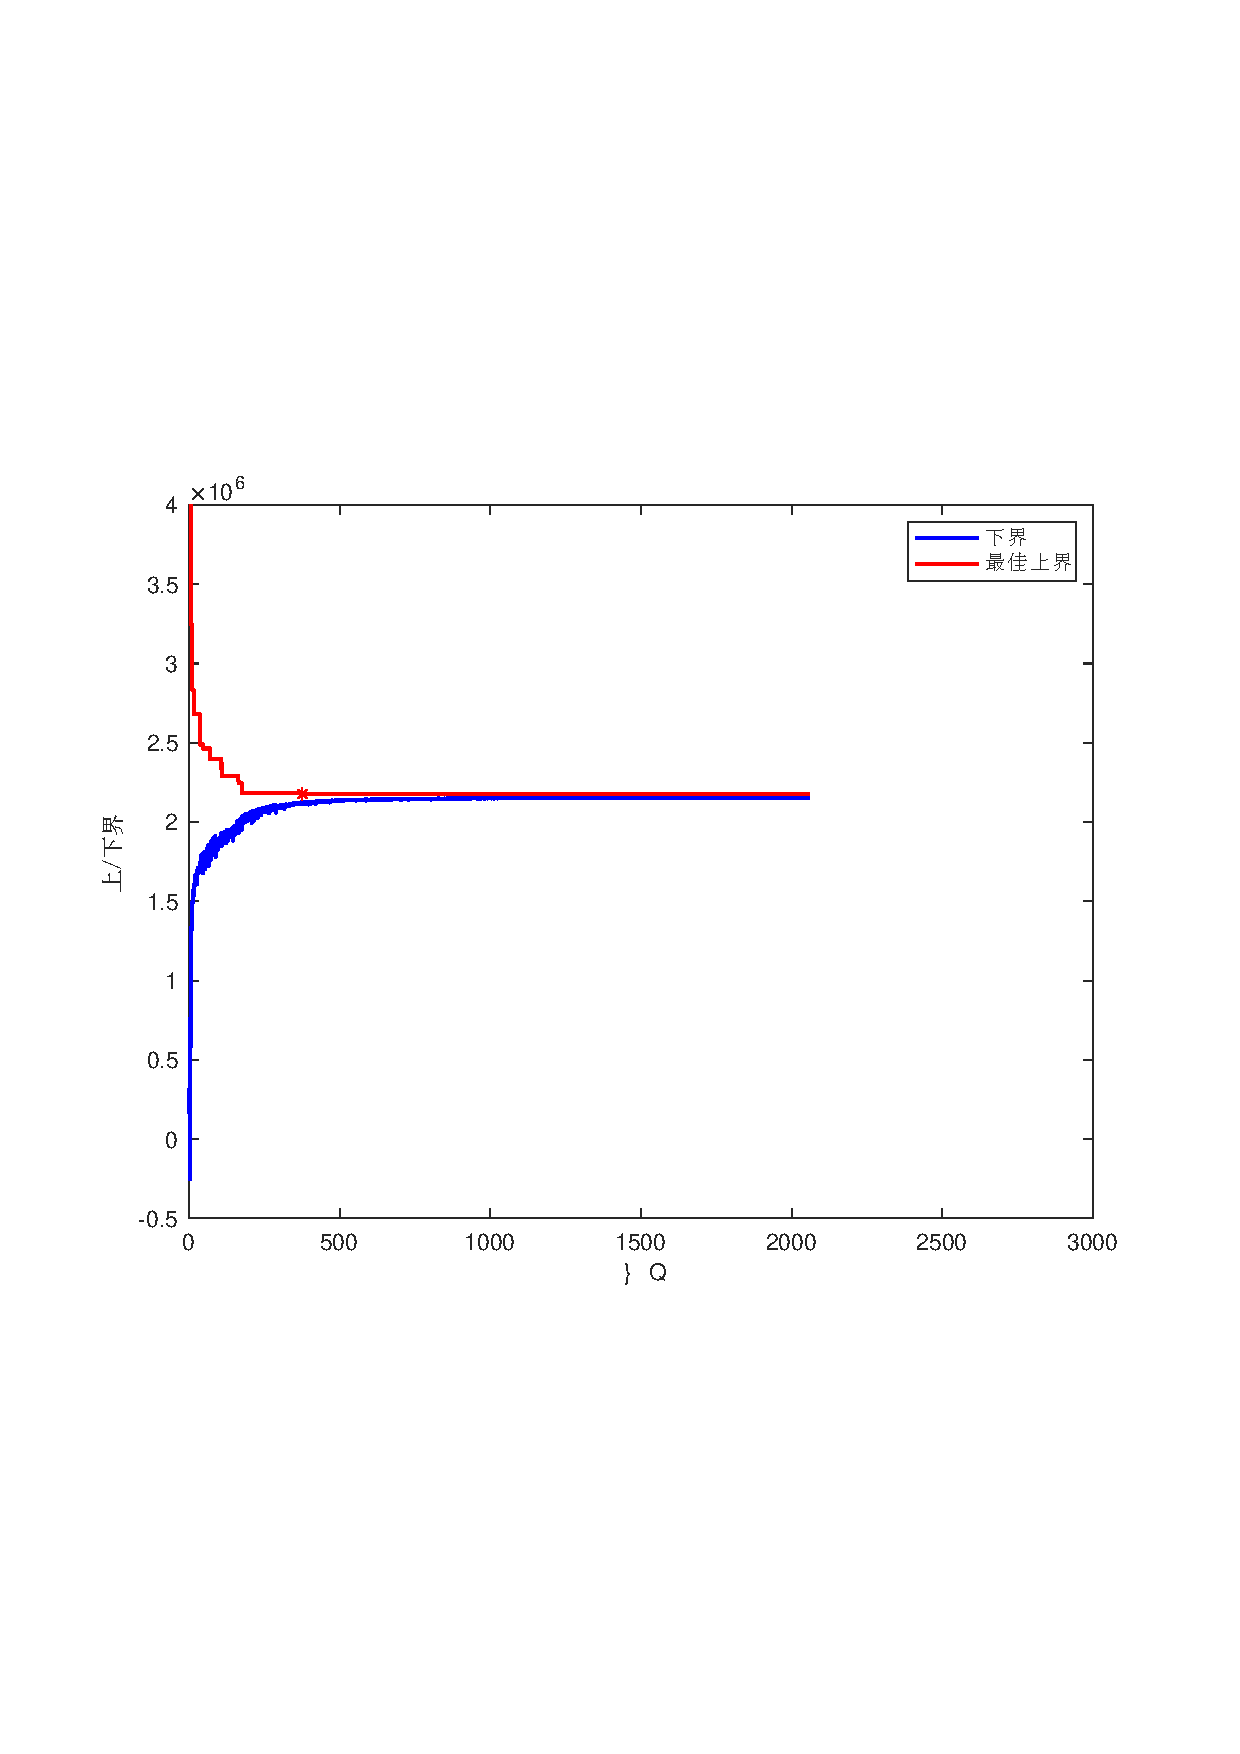
\includegraphics[width=0.47\linewidth]{figures/rslt_n150_rho0.01.pdf}}
	\quad %默认情况下两个子图之间空的较少,使用这个命令加大宽度
	\subfigure[$\rho=0.05$]{
		\label{fig:lr_sub2}
		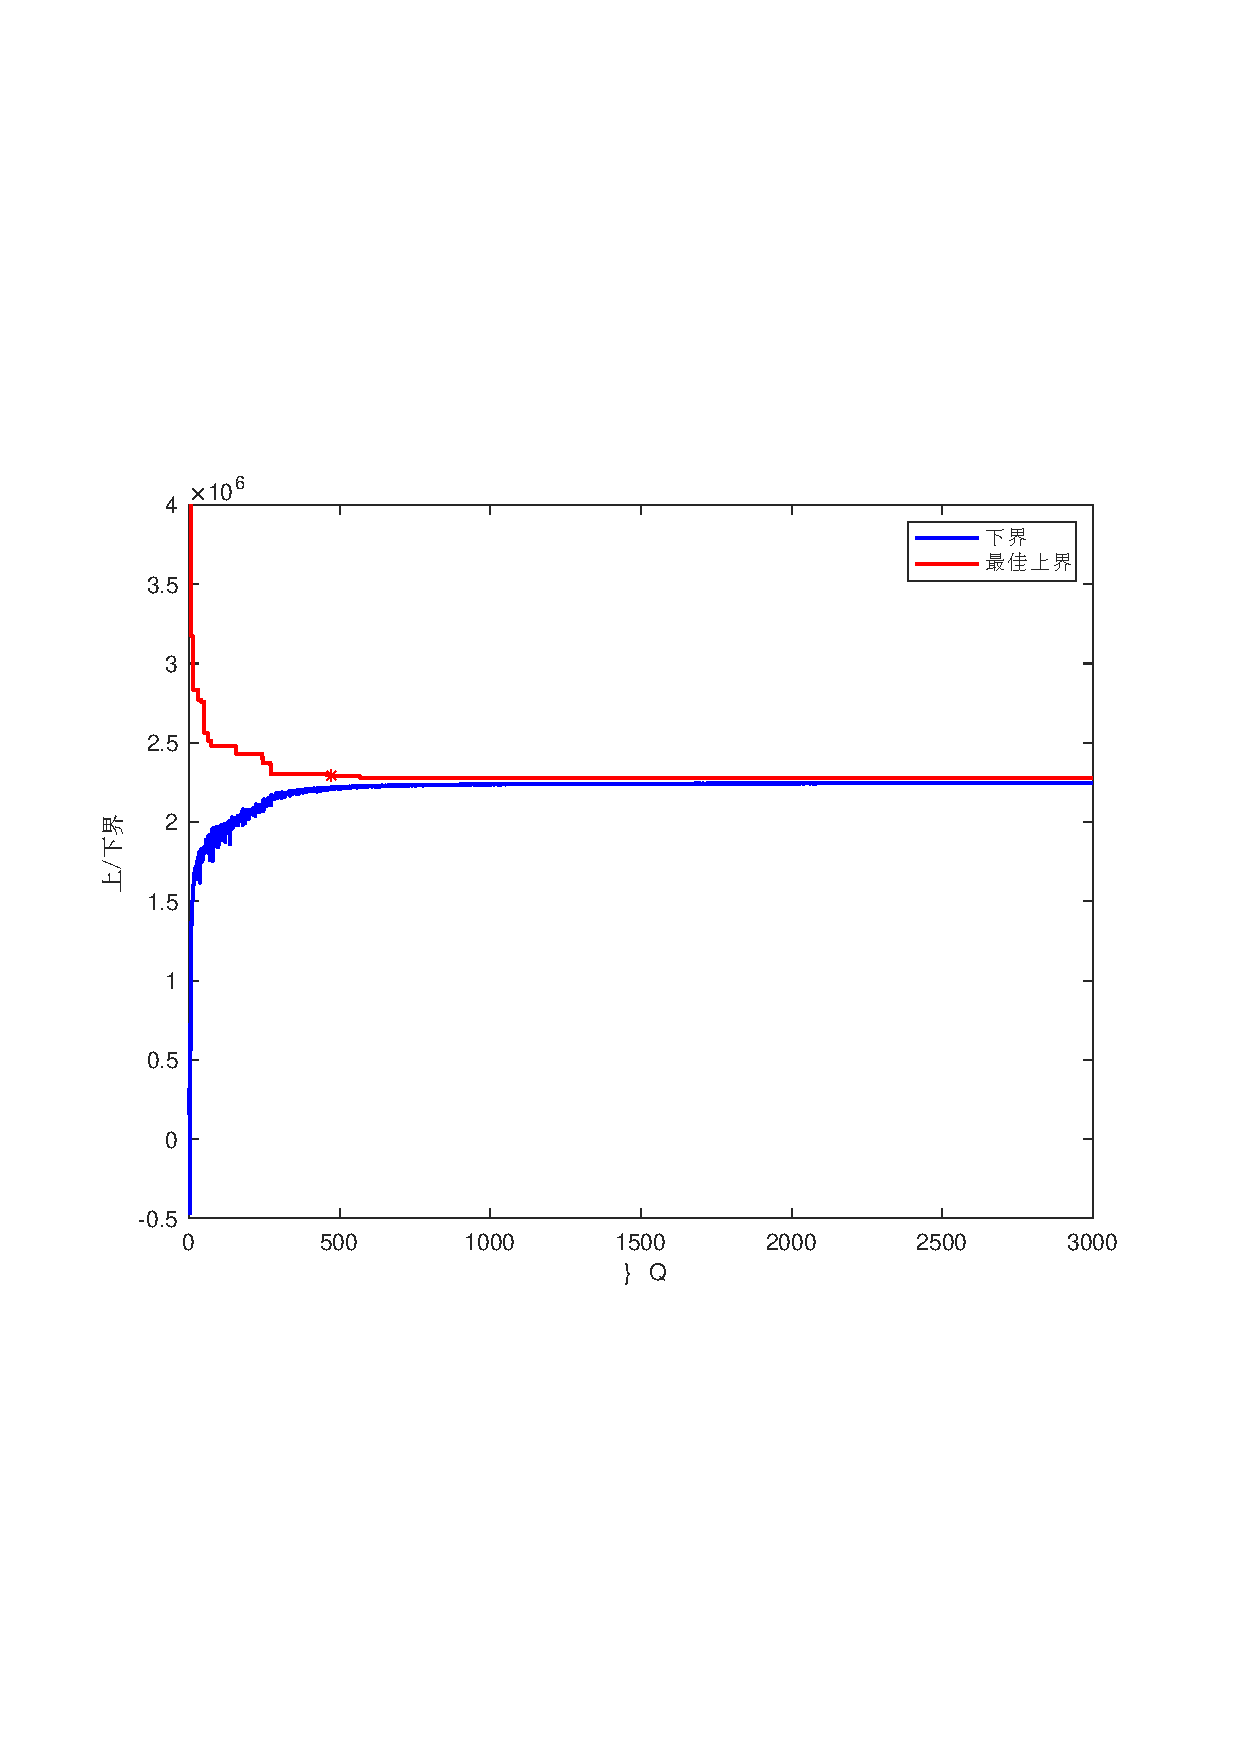
\includegraphics[width=0.47\linewidth]{figures/rslt_n150_rho0.05.pdf}}
	  %这里是空了一行,能够实现强制将四张图分成两行两列显示,而不是放不下图了再换行,使用\\也行。
	\subfigure[$\rho=0.10$]{
		\label{fig:lr_sub3}
		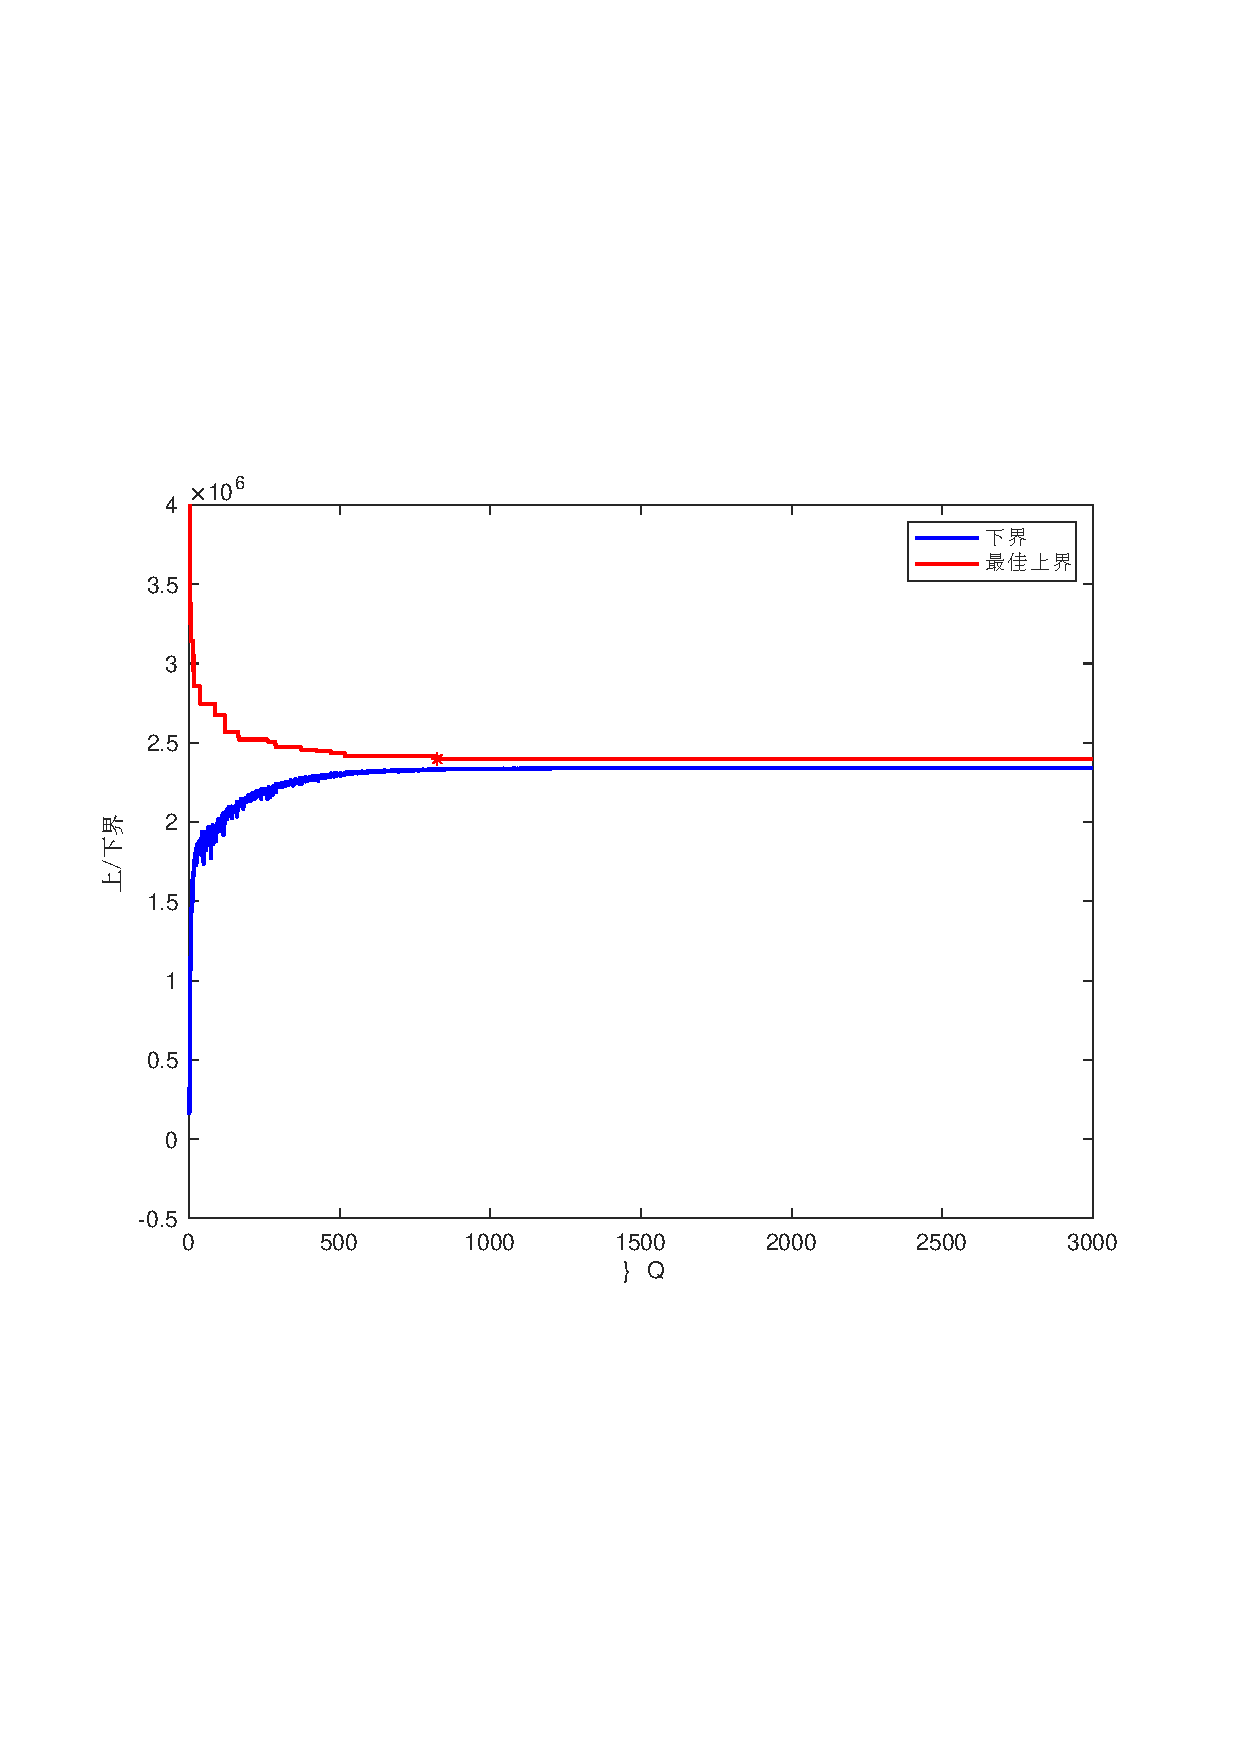
\includegraphics[width=0.47\linewidth]{figures/rslt_n150_rho0.1.pdf}}
	\quad
	\subfigure[$\rho=0.20$]{
		\label{fig:lr_sub4}
		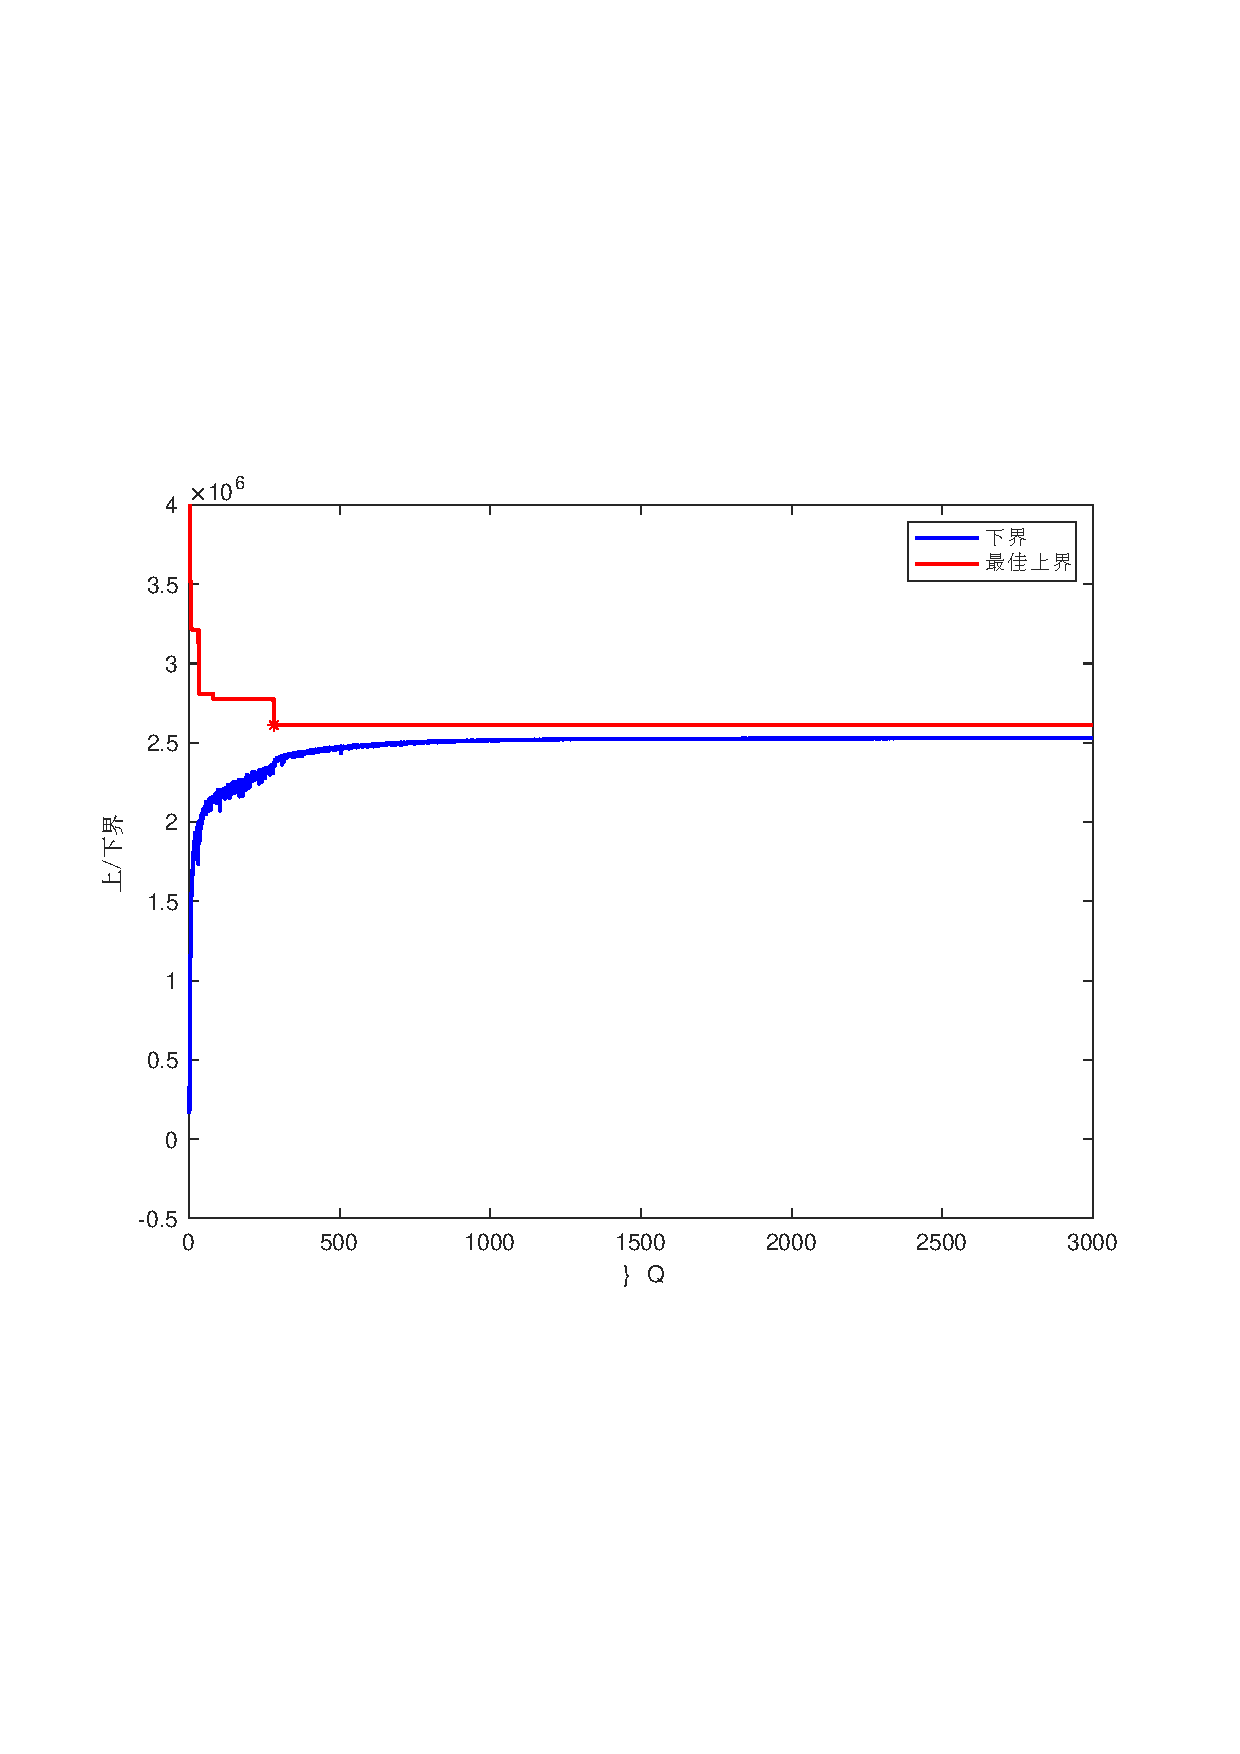
\includegraphics[width=0.47\linewidth]{figures/rslt_n150_rho0.2.pdf}}
	\caption{不同$\rho$取值的LR优化曲线\\Fig~\ref{fig:lr_curve_rho}~ LR optimization curves for different $\rho$}
	\label{fig:lr_curve_rho}
	\vspace{-0.35cm} %设置与上面正文的距离 
\end{figure}

\subsection{优化曲线}
最后,图\ref{fig:lr_curve_rho}直观展示LR-ILS算法优化过程,
使用了150个点的数据集,
默认参数$R=5$,
分别展示了了$\rho=0.01$、0.05、0.1、0.2,
不同取值的LR-ILS优化曲线。
图\ref{fig:lr_curve_rho}中,
横坐标表示迭代次数,
纵坐标表示上下界的取值;
红色的曲线表示最佳上界的变化,呈现阶梯状;
蓝色的曲线表示下界的变化,呈现锯齿状;
红色曲线上的标记表示ILS算子找到了更优的选址方案。
阶梯状上界的产生是因为LR-ILS每次迭代中仅记录最佳上界,
锯齿状下界的产生是因为迭代步长根据最佳上界值和当前下界值反复修正。
从图\ref{fig:lr_curve_rho}中可发现,算法的收敛过程相对较快,
可在500至1000次迭代内找到150个点的近似最优解,
然后下界不断提升证明其质量。
从图中可发现,
ILS可以改进上界,借助其搜索能力,
很容易根据当前上界解找到更优上界解,
进一步改进上界。
LR-ILS的大部分迭代过程在证明上界的质量,
优质上界主要由子模型RM$(\mu)_{sub1}$提供,
ILS算子的改进过程起到辅助作用。

\section{下界求解性能分析}
\label{sec:下界性能}
本节将分析算法中启发式与DFS算法求解下界解的性能,
由于构造启发式的时间复杂度优于插入启发式算法(第\ref{subsec:下界获取}节),
本节仅测试了插入启发式配合DFS算法求解下界的能力。
实验采用49个点的数据集,
$\rho$的值分别取$0.1$, $0.2$,$0.3$,
$R$值分别取2至10的整数,
拉格朗日乘子分别取全0、初始值与随机值,
其中随机值为0至30000之间的随机数。
仍采用Gurobi作为对比项,
Gurobi参数设置同表\ref{table:参数取值}一致。


测试结果如表\ref{table:下界性能}所示,
表中HEU表示仅使用启发式,
HEU-DFS表示使用启发式与DFS算法,
GRB表示使用Gurobi求解。
在测试得到的结果中,
HEU-DFS与GRB得到的结果为最优解,
HEU得到的结果为近似最优,
因此计算了HEU与最优值之间的差距,
并命名为gap*,求解时间的单位为秒,
HEU及HEU-DFS均为Matlab编码并转译生成的二进制文件,
采用了多线程计算。
表\ref{table:下界性能}中所有的结果均为$R$值分别取2至10的平均值,
该表的完整内容见附录B中的附表2。


\begin{table}[hbt]
	\small
	\setlength{\abovecaptionskip}{-0.05cm} %调整图片caption与正文之间的间距,table同理。可自己调整。
	\setlength{\belowcaptionskip}{-0.2cm} 
	\centering
	\renewcommand\arraystretch{1}
	\caption{下界求解性能\\Table~\ref{table:下界性能}~Performance on solving lower bound}
	% \resizebox{\linewidth}{!}{
		\begin{tabular}{crccccccc}
			\toprule
			\multirow{2}[1]{*}{\makecell[c]{乘子\\取值}} & \multicolumn{1}{c}{\multirow{2}[1]{*}{$\rho$}} & \multicolumn{2}{c}{HEU-DFS} & \multicolumn{3}{c}{HEU} & \multicolumn{2}{c}{GRB} \\
			\cmidrule(r){3-4} \cmidrule(r){5-7} \cmidrule(r){8-9}
			&       & 上界值   & 时间    & 上界值   & 时间(s) & gap*  & 上界值   & 时间(s) \\
			\midrule %[2pt]
			\multirow{3}[0]{*}{全零} & 0.1   & 224533.85 & 0.009 & 228752.63 & 0.001 & 0.42\% & 224532.63 & 85.260 \\
				  & 0.2   & 475214.35 & 0.012 & 493006.24 & 0.001 & 1.24\% & 475211.87 & 204.624 \\
				  & 0.3   & 756334.13 & 0.019 & 801825.67 & 0.000 & 2.68\% & 756331.82 & 388.021 \\
			\multirow{3}[0]{*}{初始} & 0.1   & 406887.38 & 0.002 & 411208.16 & 0.000 & 0.54\% & 406887.38 & 24.521 \\
				  & 0.2   & 702966.10 & 0.006 & 723855.37 & 0.000 & 1.92\% & 702966.10 & 120.713 \\
				  & 0.3	  & 1023301.45& 0.023 &1075474.89 & 0.000 & 3.23\% &1023301.45 & 349.158 \\ 
				%   & 0.3   & 513187.16 & 0.010 & 531729.61 & 0.001 & 1.36\% & 513185.96 & 164.628 \\
			\multirow{3}[1]{*}{随机} & 0.1   & 2077863.06 & 0.001 & 2082803.64 & 0.000 & 0.20\% & 2077863.06 & 15.280 \\
				  & 0.2   & 2570295.08 & 0.001 & 2600906.18 & 0.000 & 1.07\% & 2570295.08 & 15.393 \\
				  & 0.3   & 3066433.78 & 0.002 & 3140069.58 & 0.000 & 2.20\% & 3066433.78 & 22.739 \\
			\bottomrule
		\end{tabular}%
	% }
 	\vspace{-2ex}
	\label{table:下界性能}
\end{table}%

表\ref{table:下界性能}展示了采用三种方法求解得到的结果。
首先,分析三种方法的求解时间的差异。
尽管DFS算法并不是多项式时间算法,
但采用启发式搭配DFS算法得到的最优解的计算时间并不长,
并且随参数变动而变动的幅度较小。
而Gurobi的求解时间随参数变动而变动,
特别是随着$\rho$值升高,
Gurobi求解时间显著增长。
此外,拉格朗日乘子的取值对Gurobi的影响也十分大,
当乘子全为0时,Gurobi计算所有案例的平均时长为225.969s,
当乘子为初始值时,平均时长为164.797s,
当乘子取随机值时,平均时长为17.804s。
产生这种现象的原因是精确求解方法受参数影响较大。
当$R$值升高时,约束(\ref{eq:st_trytimes})变得松弛,
因此精确方法(Gurobi内置的各种Branch and Bound,Cutting Planes等方法)效果变差。
同理,随着$\rho$参数增加,节点失效概率参差不齐,
模型同样变得复杂。
拉格朗日乘子被视作访问节点的固定成本,
因此当乘子等于0时,求解器求解该模型相对困难,原因同上。
当乘子不等于0时,
精确方法可快速缩小可行域范围,
进而求解时间较短。
回到本文的启发式算法,
由于该算法是多项式时间算法,
因此求解时长随参数变动较小。
DFS算法虽然不是多项式时间算法,
但是剪枝过程大幅度缩短了计算所需的步骤,
与Gurobi相比是一种更有效地获取最优解的策略。

其次,分析三种方法求解结果的差异,
已知启发式搭配DFS算法和Gurobi可以获得最优解,
启发式方法可以获得近似解。
该启发式方法在$R$取值较大时、$\rho$取较小时,
表现良好。
并且受乘子取值的影响,
乘子不为零时表现良好。
分析该启发式的贪心策略可知,
算法每次将成本最小的节点增加至末尾。
当$R$值增加时,惩罚成本的比重逐渐被稀释,
使得贪心策略效果提升。
而$R$值较小时,贪心策略仅能考虑当前最优,
未能考虑最终惩罚成本的影响。
同理,当乘子不为零时,
乘子影响的贪心过程的决策,
进而提升了启发式的质量。
启发式方法获得的近似解总体质量较好(最大误差8.18\%,最小0.02\%,平均1.50\%),
但为了得到下界的最优解以证明上界的质量,
在本文算法仍使用了启发式搭配DFS的方式。
最后,值得注意的是,
尽管DFS和Gurobi都获得了最优解,
但在一些算例中,
Gurobi得到的值小于DFS方法得到的值。
经过排查,为决策变量$w_{ijk}$的值小于$10^{-6}$,
在Gurobi中认定为0。
有关Gurobi数值精度问题,
请参考Gurobi在线手册
\footnote{https:\slash \slash www.gurobi.com\slash documentation\slash 9.5\slash refman\slash guidelines\_for\_numerical\_i.html}。

\section{上界求解性能分析}
\label{sec:上界性能}

本文的第\ref{subsec:上界获取}节介绍了获取上界值的方法,
在给定选址方案$J^*$的前提下,
可很容易计算得到节点建设的固定成本,
计算客户的期望运输成本等于求解第\ref{subsec:subprob}节的客户试错序列问题。
第\ref{subsec:上界获取}节介绍的Dijkstra变种算法可以获得客户试错序列的近似解;
第\ref{subsec:上界获取}节提出可用DFS算法获得上界的最优值。
此外,还可使用Gurobi求解器求解模型的上界值。

本节对求解上界的性能进行了测试,
分别使用了Dijkstra变种算法(本节简称为DIJK),
Dijkstra变种算法搭配DFS算法(本节简称为DIJK-DFS),
以及Gurobi求解器(本节简称为GRB)求解了49个点的不同算例。
已知选址方案$J^*$中设施的个数显著影响算法求解时长,
因此,本节分别测试了10,20,30,40个点的选址方案,
参数$\rho$取值0.1,0.2,0.3,
参数$R$取值为大于等于2小于等于10的整数。
测试结果如表\ref{table:上界性能}所示,
表中近似解与最优之间的差距命名为gap*。
求解时间单位为秒,
DIJK算法与DIJK-DFS算法均为Matlab编码并转译成C++二进制文件,
采用了多线程计算。
表\ref{table:上界性能}中所有的结果均为$R$值分别取2至10的平均值,
该表的完整内容见附录B中的附表3。
 

\begin{table}[hbt]
	\small
	\setlength{\abovecaptionskip}{-0.05cm} %调整图片caption与正文之间的间距,table同理。可自己调整。
	\setlength{\belowcaptionskip}{-0.2cm} 
	\centering
	\renewcommand\arraystretch{1}
	\caption{上界求解性能\\Table~\ref{table:上界性能}~Performance on solving upper bound}
		\begin{tabular}{crccccccc}
			\toprule
			\multirow{2}[1]{*}{\makecell[c]{$|J^*|$}} & \multicolumn{1}{c}{\multirow{2}[1]{*}{$\rho$}} & \multicolumn{2}{c}{DIJK-DFS} & \multicolumn{3}{c}{DIJK} & \multicolumn{2}{c}{GRB} \\
			\cmidrule(r){3-4} \cmidrule(r){5-7} \cmidrule(r){8-9}
			&       & 上界值   & 时间    & 上界值   & 时间(s) & gap*  & 上界值   & 时间(s) \\
			\midrule %[2pt]
			\multirow{3}[0]{*}{10} 	& 0.1   & 1611587.91 & 0.001 & 1640555.97 & 0.006 & 1.90\% & 1611590.82 & 5.111 \\
									& 0.2   & 1925003.60 & 0.001 & 2011904.94 & 0.001 & 4.68\% & 1925001.32 & 5.803 \\
									& 0.3   & 2287526.81 & 0.001 & 2472292.62 & 0.001 & 8.35\% & 2287525.39 & 6.340 \\
	 		\multirow{3}[0]{*}{20} 	& 0.1   & 2067339.22 & 0.001 & 2072951.15 & 0.001 & 0.22\% & 2067342.67 & 10.999 \\
									& 0.2   & 2335167.39 & 0.002 & 2371565.20 & 0.001 & 1.39\% & 2335168.60 & 11.597 \\
									& 0.3   & 2639304.64 & 0.002 & 2750515.28 & 0.001 & 4.01\% & 2639302.63 & 14.668 \\
	  		\multirow{3}[0]{*}{30} 	& 0.1   & 2752865.35 & 0.003 & 2761269.07 & 0.001 & 0.22\% & 2752853.58 & 19.238 \\
									& 0.2   & 3011919.92 & 0.006 & 3097686.57 & 0.001 & 2.61\% & 3011907.14 & 25.567 \\
									& 0.3   & 3305273.39 & 0.006 & 3490345.05 & 0.001 & 5.16\% & 3305262.35 & 45.998 \\
	  		\multirow{3}[0]{*}{40} 	& 0.1   & 3323545.36 & 0.004 & 3331937.55 & 0.001 & 0.20\% & 3323545.56 & 48.869 \\
									& 0.2   & 3575894.34 & 0.006 & 3640638.02 & 0.001 & 1.66\% & 3575893.29 & 84.519 \\
									& 0.3   & 3858144.43 & 0.017 & 4031583.03 & 0.001 & 4.25\% & 3858140.97 & 156.080 \\
			\bottomrule
		\end{tabular}%
 	\vspace{-2ex}
	\label{table:上界性能}
\end{table}%


表\ref{table:上界性能}展示了使用三种方法求解上界的结果,
从求解时间的角度分析,
对比Gurobi求解器,
DIJK算法以及DIJK-DFS算法具有显著优势。
对于所有算例,上述两种算法可以在0.1秒内给出上界值,
而Gurobi虽然可以获得上界值,
但求解时间明显与这两种算法不在同一数量级
(最小差距1131.29倍,最大差距63136.36倍,详见附表3)。
并且Gurobi的求解时间随参数变动而变动,
$|J^*|$越大、参数$\rho$越大、参数$R$越大,
则模型越复杂,导致Gurobi求解时间越长。
最短可在几秒内完成简单算例的求解,
最长需要几分钟。
DIJK算法以及DIJK-DFS算法求解时间则非常稳定,
最长不超过0.1秒。
Gurobi求解时长随参数变化的原因已在第\ref{sec:下界性能}节分析。

已知在本测试中,
Gurobi和DIJK-DFS获得上界的最优值,
但DIJK算法只能获得近似值。
表\ref{table:上界性能}的gap*列
展示了该算法获得的近似上界值和最优值之间的相对差距,
在$R$值较大时,DIJK算法得到的解质量较好。
但在$R$值较小时,DIJK算法算法表现劣化。
DIJK算法是基于Dijkstra算法进行了问题的适配,
但保留了Dijkstra算法永久标号的主要想法,
所以不可修改的标号将在$R$值较小时生成质量欠佳的决策,
进而影响解的质量。
当$R$值较大时,即便初始步骤生成的路径质量欠佳,
可通过后续决策降低惩罚成本的比重。
即便DIJK算法求解$R$值较小的问题的效果较差,
但DFS算法在$R$值较小时因搜索深度较小而展现了良好的性能。

综上,求解上界的Dijkstra变种算法在求解$R$值较小的问题时,
得到的上界质量较差,但DFS算法的搜索深度较浅,
可快速基于Dijkstra变种算法的解获得最优解。
在$R$值较大时,Dijkstra变种算法得到的上界质量较好,
为DFS算法提供了一个质量较好的已知解,
加速了DFS中剪枝的过程。
两种算法优势互补,使求解上界的过程十分有效。


\section{乘子更新效果讨论}
\label{sec:乘子性能}
本文的第\ref{subsec:乘子更新}小节阐述了拉格朗日乘子初始设置以及乘子更新的方法,
本节将对比多种乘子初始化方法以及两种乘子更新方法的不同效果。
为了显著体现不同拉格朗日乘子设置产生的效果,
本节使用了相对较小的49个点的数据集进行实验,
对比分析拉格朗日优化曲线的收敛性。
在本节中,默认设置参数$R=5$,
参数$\rho$分别取值0.05、0.1、0.2、0.3。
为了消除其他因素的干扰,
本节的所有测试均关闭了ILS算子。

\begin{figure}[!t] %这里使用的是强制位置,除非真的放不下,不然就是写在哪里图就放在哪里,不会乱动
	\centering  %图片全局居中
	\vspace{-0.35cm} %设置与上面正文的距离
	\subfigtopskip=2pt %设置子图与上面正文或别的内容的距离
	\subfigbottomskip=2pt %设置第二行子图与第一行子图的距离,即下面的头与上面的脚的距离
	\subfigcapskip=-5pt %设置子图与子标题之间的距离
	\subfigure[$\rho=0.05$]{
		\label{fig:mp_sub1}
		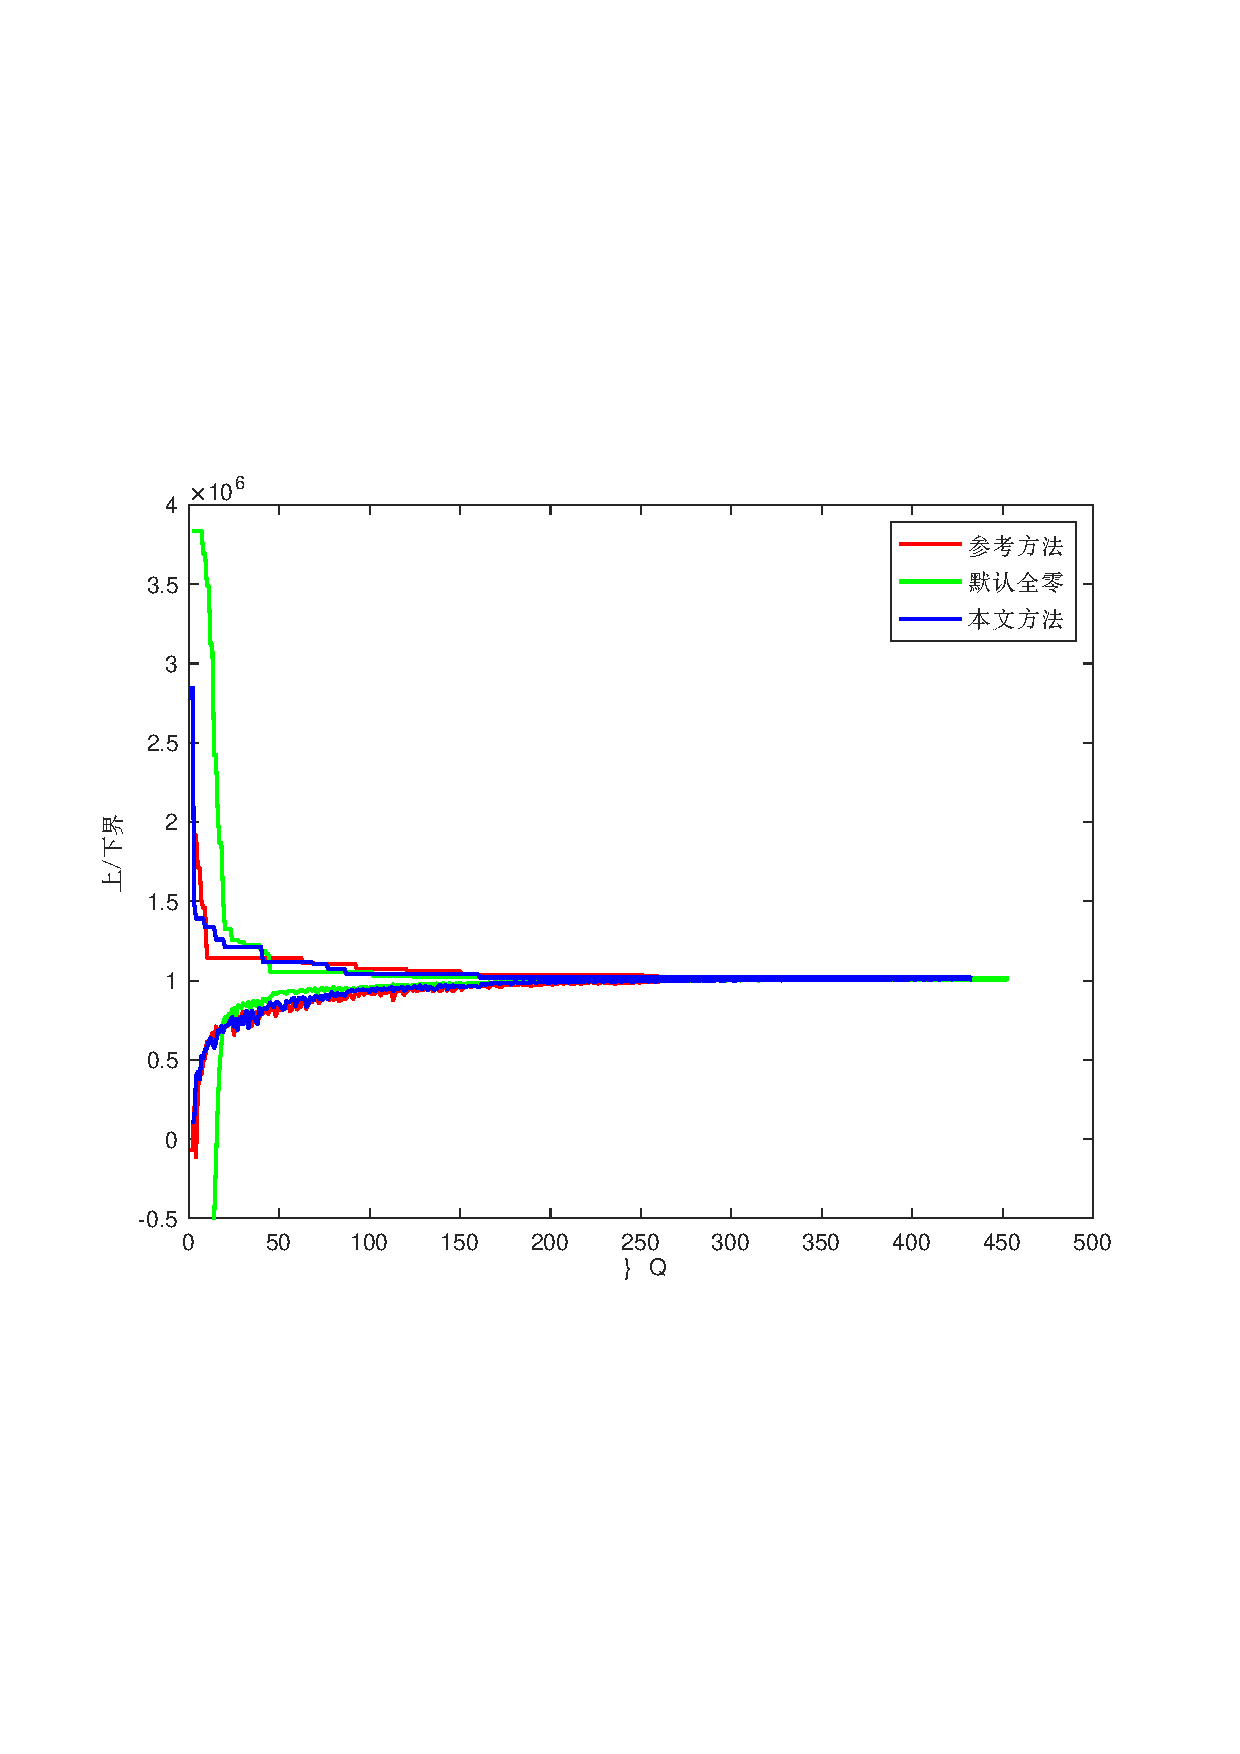
\includegraphics[width=0.47\linewidth]{figures/result_mp_rho0.05.pdf}}
	\quad %默认情况下两个子图之间空的较少,使用这个命令加大宽度
	\subfigure[$\rho=0.1$]{
		\label{fig:mp_sub2}
		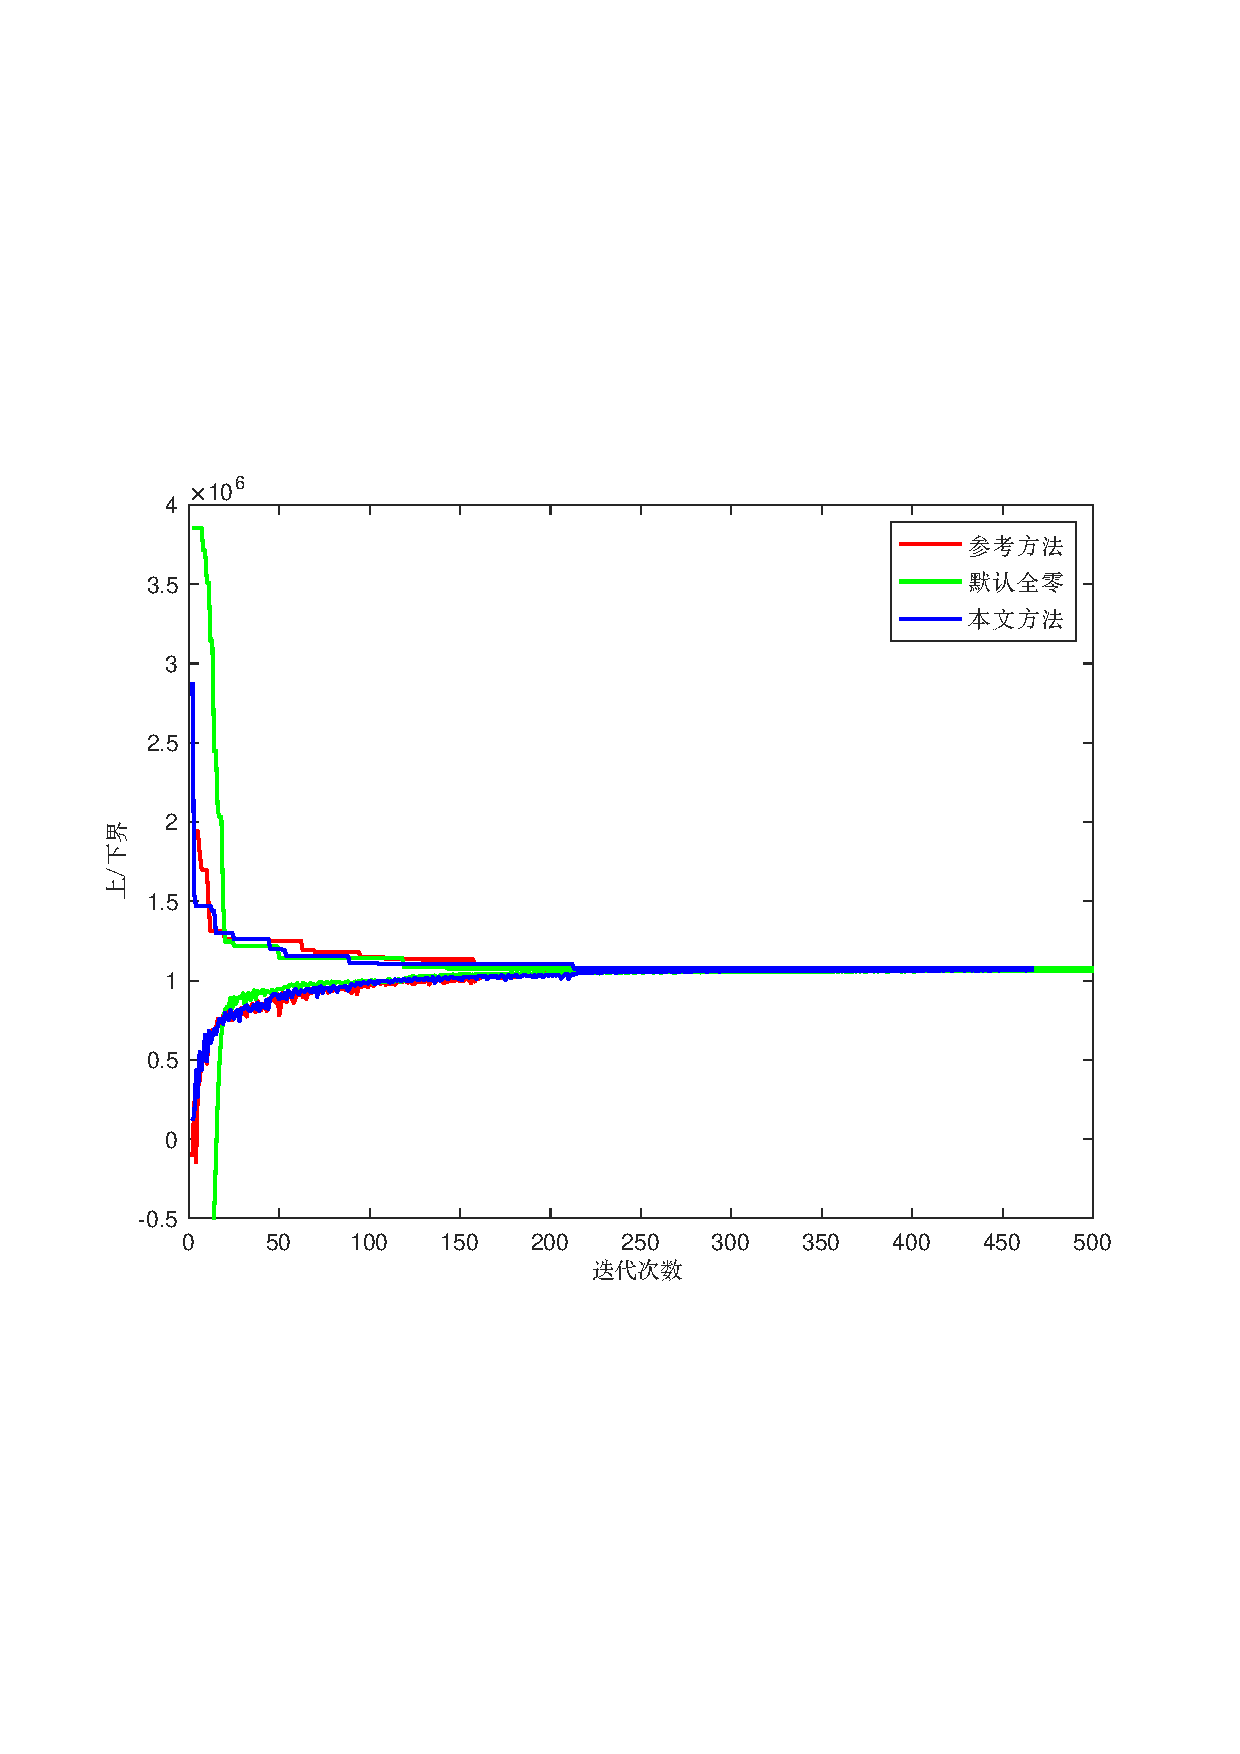
\includegraphics[width=0.47\linewidth]{figures/result_mp_rho0.1.pdf}}
	  %这里是空了一行,能够实现强制将四张图分成两行两列显示,而不是放不下图了再换行,使用\\也行。
	\subfigure[$\rho=0.2$]{
		\label{fig:mp_sub3}
		% \includegraphics[width=0.47\linewidth]{figures/result_mp_rho0.2.eps}}
		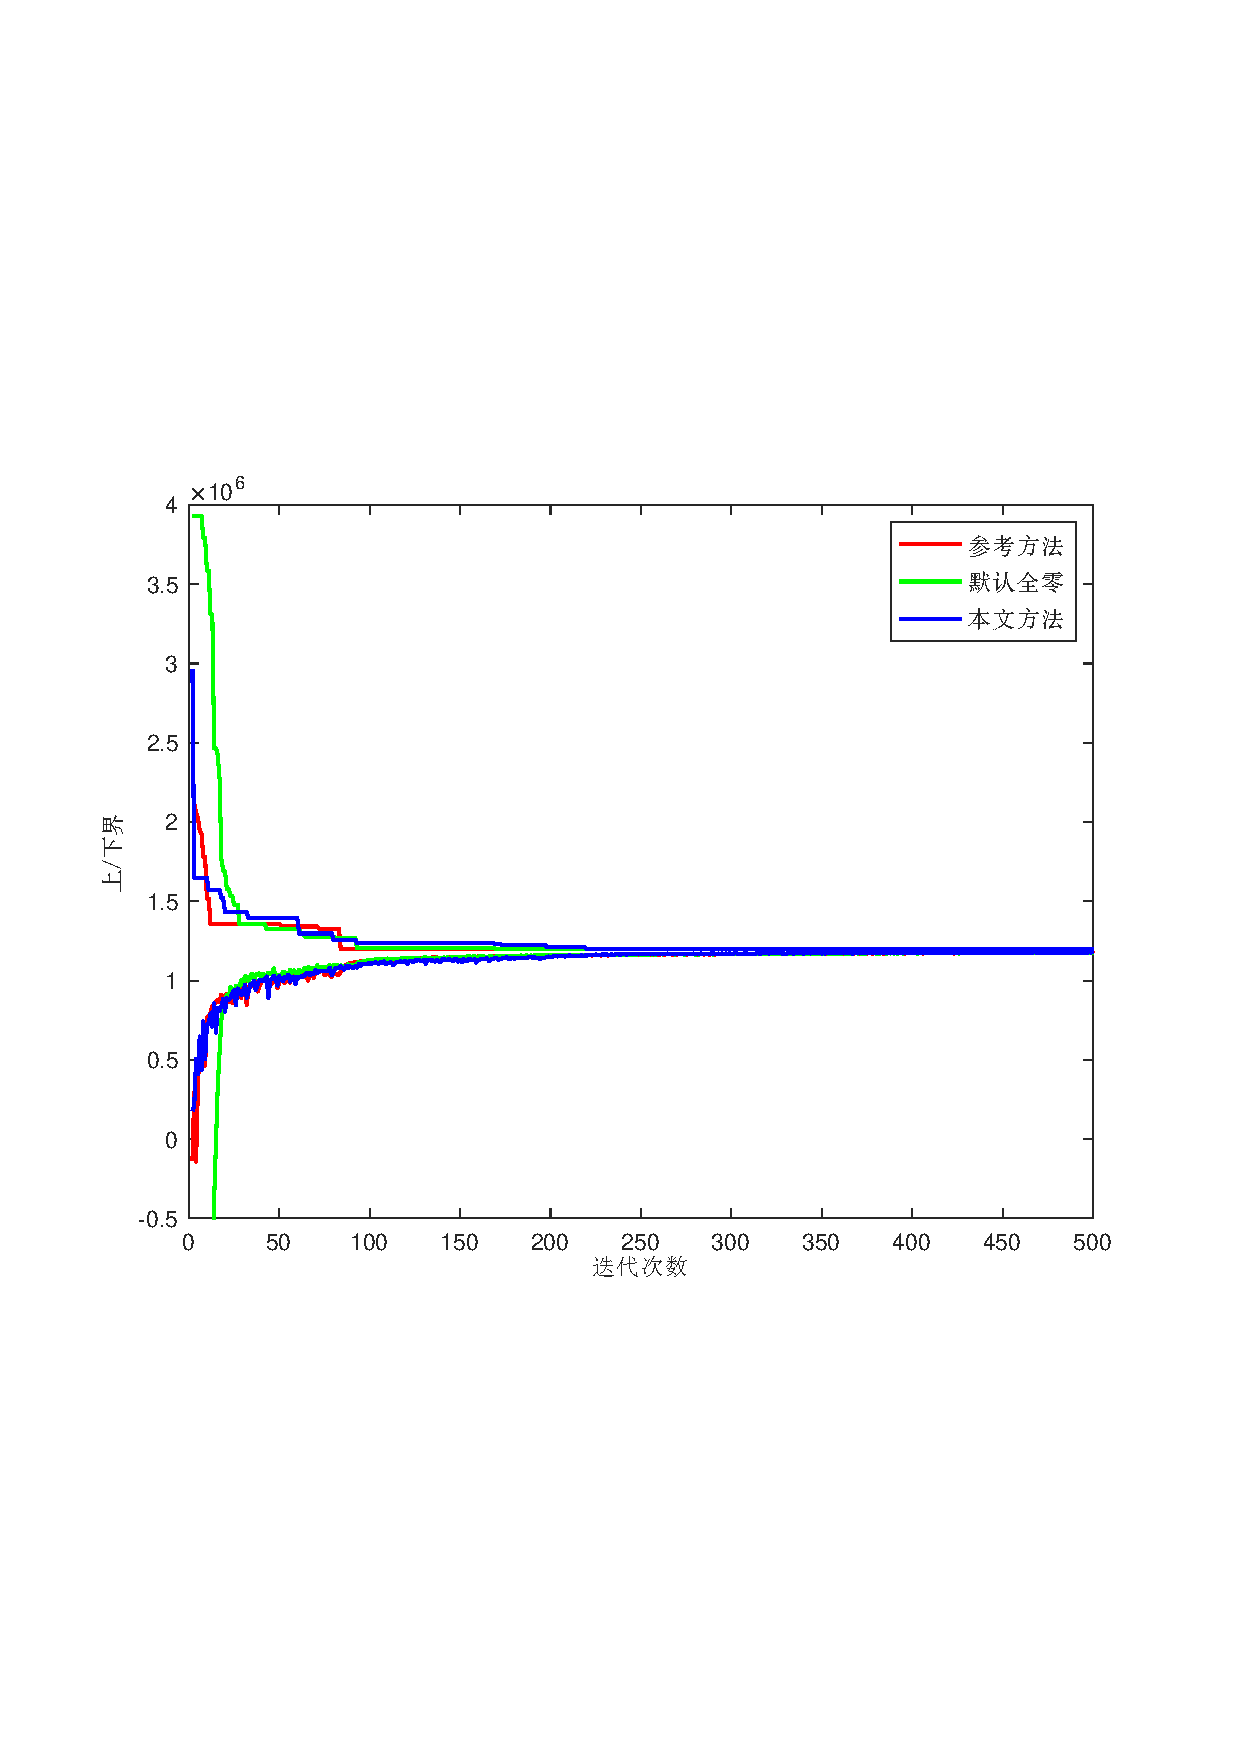
\includegraphics[width=0.47\linewidth]{figures/result_mp_rho0.2.pdf}}
	\quad
	\subfigure[$\rho=0.3$]{
		\label{fig:mp_sub4}
		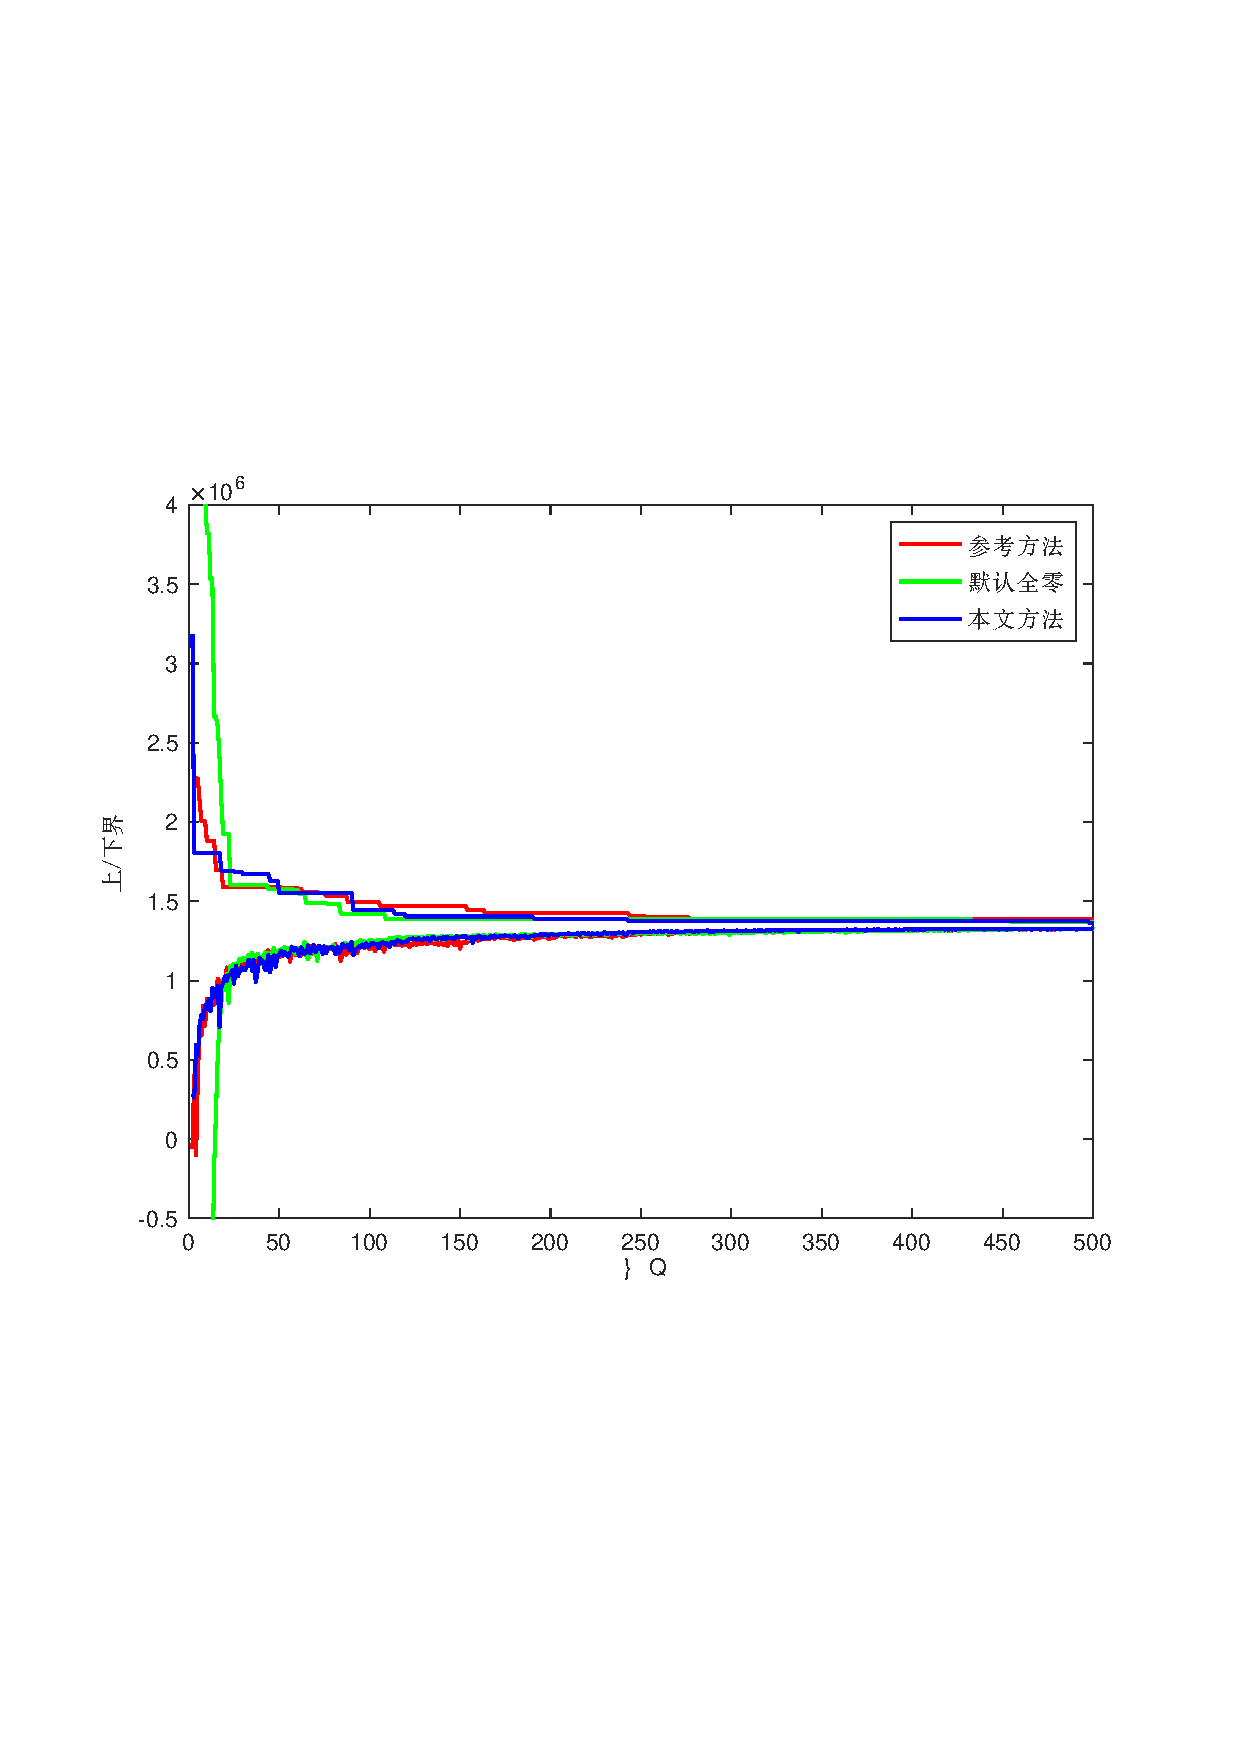
\includegraphics[width=0.47\linewidth]{figures/result_mp_rho0.3.pdf}}
	\caption{乘子初始值的不同策略对优化过程的影响\\Fig~\ref{fig:mp_curves}~ Effect of initialization strategies of the multiplier on the optimization process}
	\label{fig:mp_curves}
	\vspace{-0.35cm} %设置与上面正文的距离
\end{figure}

图\ref{fig:mp_curves}中展示了在不同$\rho$取值的情况下,
算法前500次迭代的结果。
图中绿色曲线表示将全部乘子初始值设置成0的结果,
红色表示文献\cite{yun2015}使用的乘子初始化方法,
蓝色曲线表示本文使用的乘子初始化方法。
从整体优化的趋势来看,
三种方法的优化曲线都呈现良好的收敛趋势,
最终上下界都收敛只最优解附近。
然而,效果最差的初始乘子方法是默认全零方法,
该方法的初始gap值非常大,
并且在$\rho=0.05$的情况下迭代次数最多。
虽然该方法的前期gap值非常差,
但可以快速收敛,
并且在所有测试中下界收敛效果最好。
对比文献\cite{yun2015}的方法,
本文的方法在LR迭代的第一次迭代时得到的上界更大,
但可以快速下降。
本文方法获得的上界结果不如文献\cite{yun2015}的方法,
但获取下界的效果更好,
体现在下界初始波动更小,
获得的下界值更高。
为了方便展示优化曲线的主体部分,
图\ref{fig:mp_curves}忽略了默认全零方法前几次迭代的下界结果,
该下界结果的量级在$-10^{7}$左右。
相比之下,其他两种方法的初始下界均在0附近。

得益于良好的迭代策略,
三种方法最后都收敛于最优解附近。
公式(\ref{eq:steplen})展示了拉格朗日乘子步长设置的准则,
对基础乘子更新策略中迭代步长进行了改进,
取消了分母的二次项并设置为一次项。

图\ref{fig:step_curves}展示了算法两种不同乘子更新策略的结果,
同样以49个点的为基准进行测试,
其中默认$R=5$,
参数$\rho$分别取值0.05、0.1、0.2、0.3。
图中红色的曲线表示若公式(\ref{eq:steplen})分母项取二次(即原始步长公式)获得的上下界迭代效果,
蓝色曲线表示公式(\ref{eq:steplen})(即本文使用的改进公式)的效果。
显然,无论是收敛性还是上下界质量,
使用改进公式的效果都十分明显。
产生这样的差异的原因是,
当公式(\ref{eq:steplen})的分母取平方项时,
生成的迭代步长过小,
每次迭代对拉格朗日乘子的修正较小,
因此获取上下界的效果较差。
改进的公式取消了平方操作,
每次迭代的步长较大,乘子更新更为激进,
进而得到了良好的效果。


\begin{figure}[htb] %这里使用的是强制位置,除非真的放不下,不然就是写在哪里图就放在哪里,不会乱动
	\centering  %图片全局居中
	\vspace{-0.35cm} %设置与上面正文的距离
	\subfigtopskip=2pt %设置子图与上面正文或别的内容的距离
	\subfigbottomskip=2pt %设置第二行子图与第一行子图的距离,即下面的头与上面的脚的距离
	\subfigcapskip=-5pt %设置子图与子标题之间的距离
	\subfigure[$\rho=0.05$]{
		\label{fig:step_sub1}
		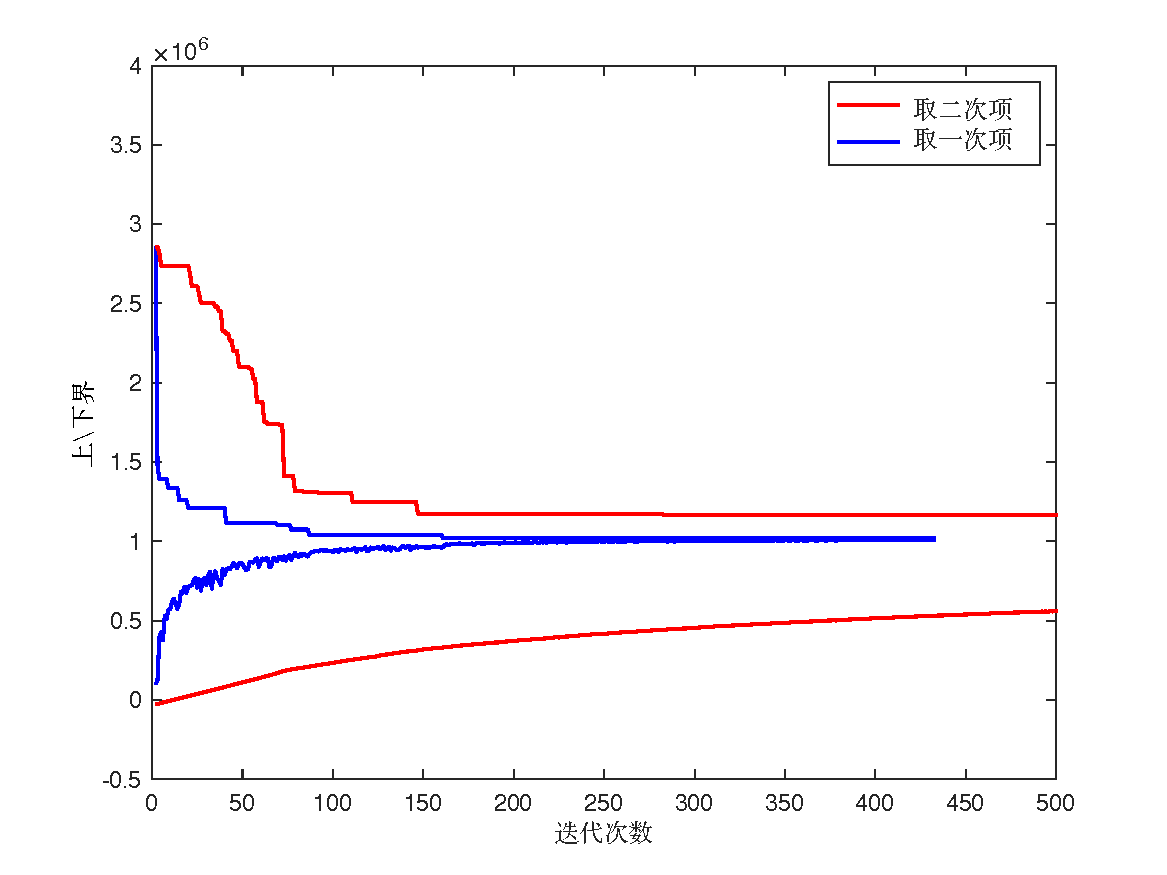
\includegraphics[width=0.47\linewidth]{figures/result_mu_update0.05.pdf}}
	\quad %默认情况下两个子图之间空的较少,使用这个命令加大宽度
	\subfigure[$\rho=0.1$]{
		\label{fig:step_sub2}
		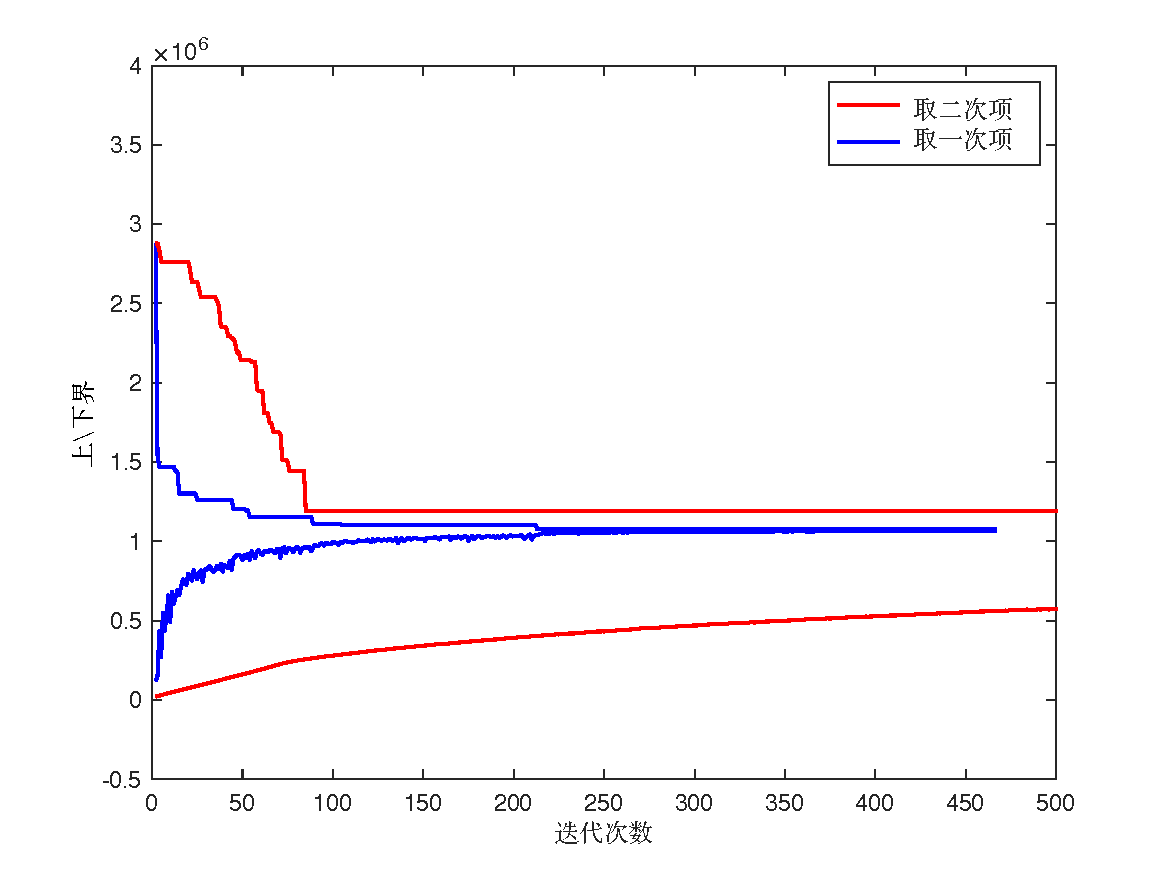
\includegraphics[width=0.47\linewidth]{figures/result_mu_update0.1.pdf}}
	  %这里是空了一行,能够实现强制将四张图分成两行两列显示,而不是放不下图了再换行,使用\\也行。
	\subfigure[$\rho=0.2$]{
		\label{fig:step_sub3}
		% \includegraphics[width=0.47\linewidth]{figures/result_mp_rho0.2.eps}}
		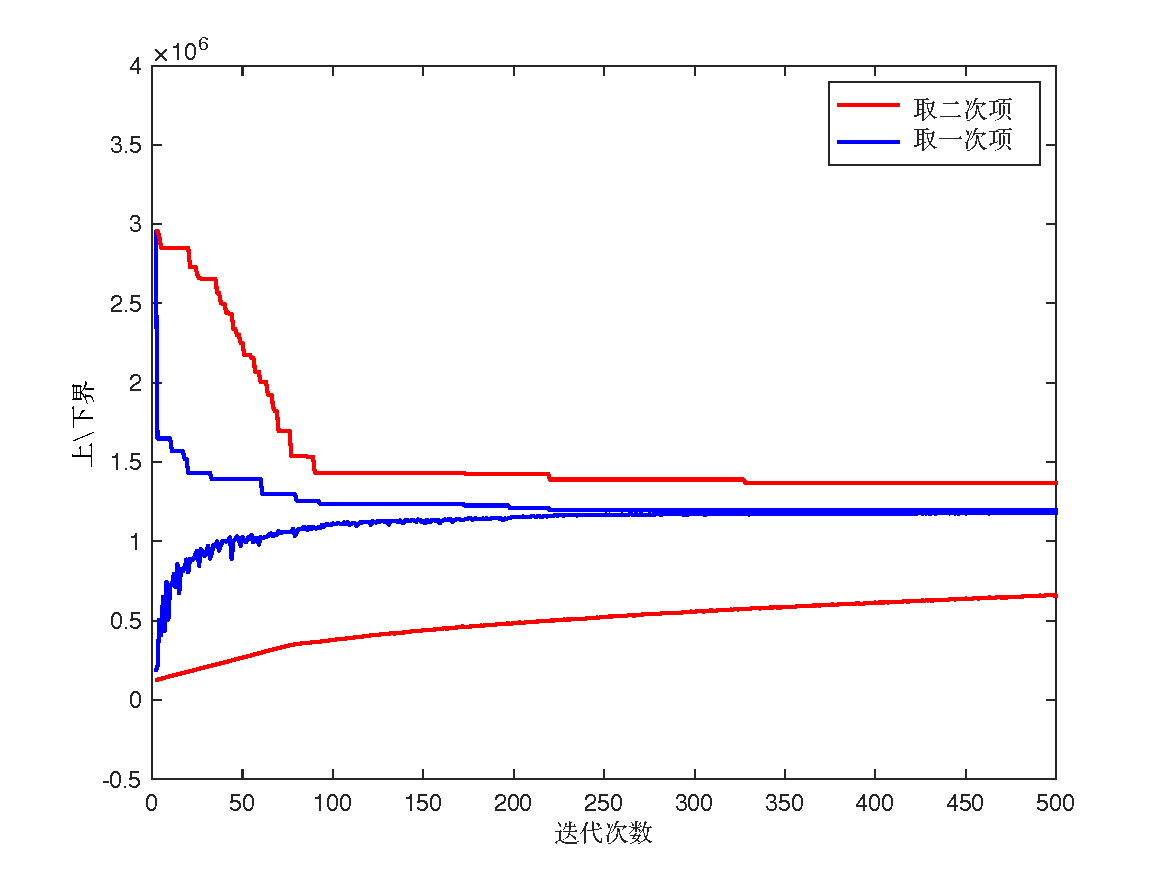
\includegraphics[width=0.47\linewidth]{figures/result_mu_update0.2.pdf}}
	\quad
	\subfigure[$\rho=0.3$]{
		\label{fig:step_sub4}
		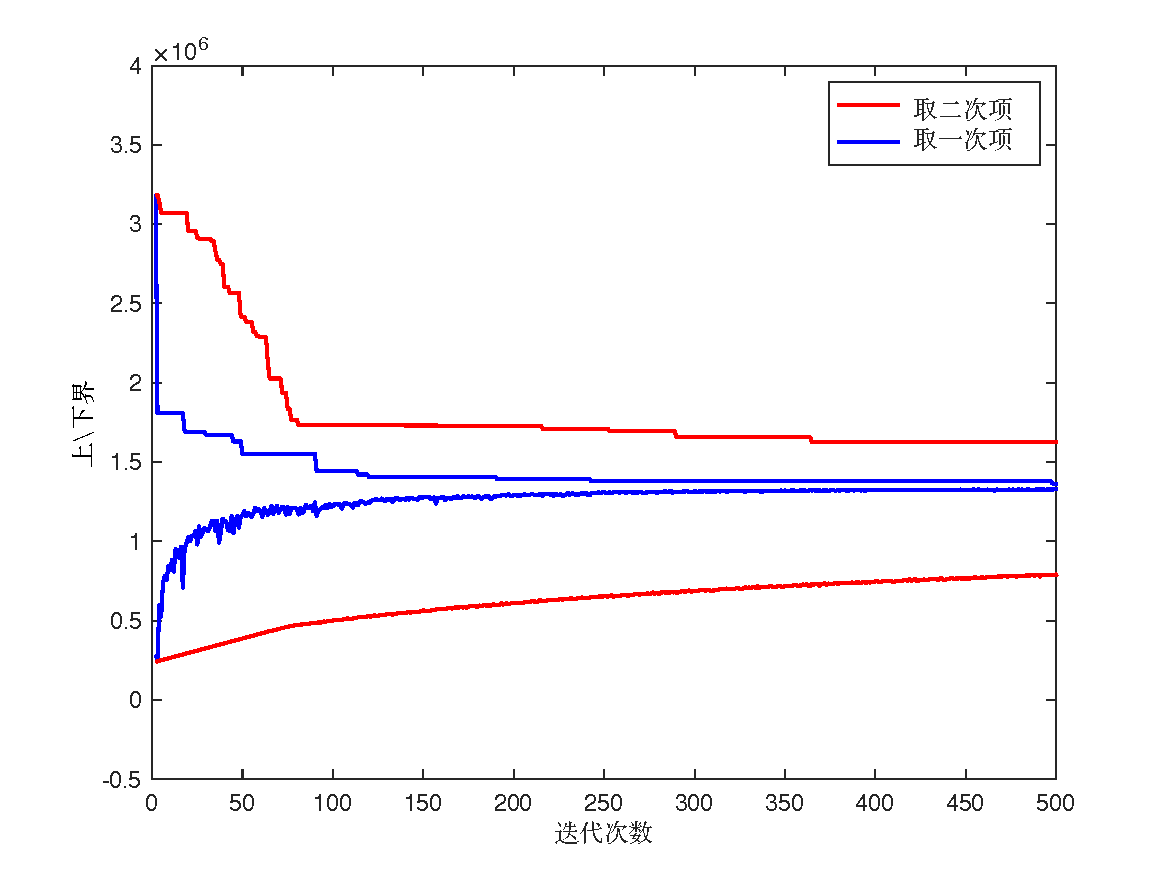
\includegraphics[width=0.47\linewidth]{figures/result_mu_update0.3.pdf}}
	\caption{迭代步长对优化过程的影响\\Fig~\ref{fig:step_curves}~ Effect of step length strategies of the multiplier on the optimization process}
	\label{fig:step_curves}
	\vspace{-0.35cm} %设置与上面正文的距离
\end{figure}


\section{线性化效果讨论}
\label{sec:线性化优势}

本文的第\ref{sec:线性化}节提出了模型的线性化方法,
该方法消除了模型中的二次项,
在理想情况下可降低采用精确方法求解问题的难度。
本节将对比使用Gurobi求解线性模型和非线性模型的性能差距。
求解器参数设置同表\ref{table:参数取值}一致,
测试了15个点的小规模数据集,
其来源于49个点的数据集的前15个点。
设置参数$\rho$分别等于0.05,0.1,0.2,0.3,
参数$R$为大于等于2小于等于10的整数,
求解结果如表\ref{table:线性化结果}所示。
表中上界值为模型的目标函数值,
即目标函数(\ref{eq:obj_model})和目标函数(\ref{eq:l_obj_model}),
gap值为Gurobi返回的gap结果,
求解时间为Gurobi求解时长(秒)。


从表\ref{table:线性化结果}的结果综合来看,
使用Gurobi求解器求解线性模型和非线性模型的困难程度相差不大。
在上述测试中,求解线性模型的平均时间为494.35秒,
求解非线性模型的平均时间为469.79秒;
求解线性模型平均gap值为1.82\%,
非线性模型平均gap值为1.87\%。
对于小规模的15个点的问题,
当参数$\rho$较小时,
求解线性模型相对容易,
当参数$\rho$较大时,
线性化的作用并不明显,
在某些数据测试中,求解线性模型较为简单,
在其他数据测试中,求解非线模型较为简单。

{ \small
\begin{longtable}{ccrrrrrr}
	\caption{非线性模型和线性模型求解结果对比\\Table~\ref{table:线性化结果}~Comparing the results of solving the linear and non-linear models}
    \label{table:线性化结果} \\ % add \\ command to tell LaTeX to start a new line
 
    % Appear table header at the first page as well
    \toprule
	\multirow{2}[0]{*}{$\rho$} & \multirow{2}[0]{*}{$R$} & \multicolumn{3}{c}{非线性模型} & \multicolumn{3}{c}{线性模型} \\
	\cmidrule(r){3-5} \cmidrule(r){6-8}
	&       & \multicolumn{1}{c}{上界值} & \multicolumn{1}{c}{gap} & \multicolumn{1}{c}{时长(s)} & \multicolumn{1}{c}{上界值} & \multicolumn{1}{c}{gap} & \multicolumn{1}{c}{时长(s)} \\
    
	\hline
    \endfirsthead
 
    % Appear the table header at the top of every page
	\multicolumn{8}{r}%
	{{(续\tablename\thetable{})}} \\
    \toprule
	\multirow{2}[0]{*}{$\rho$} & \multirow{2}[0]{*}{$R$} & \multicolumn{3}{c}{非线性模型} & \multicolumn{3}{c}{线性模型} \\
	\cmidrule(r){3-5} \cmidrule(r){6-8}
	&       & \multicolumn{1}{c}{上界值} & \multicolumn{1}{c}{gap} & \multicolumn{1}{c}{时长(s)} & \multicolumn{1}{c}{上界值} & \multicolumn{1}{c}{gap} & \multicolumn{1}{c}{时长(s)} \\
	\hline
	\endhead 
 
    % Appear \hline at the bottom of every page
    \hline
	\multicolumn{3}{l}{{(接续\tablename\ \thetable{})}} \\ 
    \endfoot 
	
	\hline
	\endlastfoot
    % data begins here]
	% Table generated by Excel2LaTeX from sheet '线性化'

			& 2     & 1184928.86 & 0.00\% & 0.07  & 1184928.86 & 0.00\% & 0.08 \\
			& 3     & 664900.02 & 0.00\% & 3.48  & 664900.02 & 0.00\% & 2.83 \\
			& 4     & 644206.22 & 0.00\% & 6.02  & 644206.22 & 0.00\% & 5.47 \\
			& 5     & 643430.51 & 0.00\% & 5.55  & 643430.51 & 0.00\% & 4.52 \\
	  0.05  & 6     & 643401.30 & 0.00\% & 6.55  & 643401.87 & 0.00\% & 4.22 \\
			& 7     & 643401.56 & 0.00\% & 6.03  & 643401.17 & 0.00\% & 3.70 \\
			& 8     & 643401.34 & 0.00\% & 4.57  & 643402.93 & 0.00\% & 3.57 \\
			& 9     & 643409.86 & 0.00\% & 6.67  & 643401.18 & 0.00\% & 3.97 \\
			& 10    & 643401.32 & 0.00\% & 5.30  & 643401.11 & 0.00\% & 5.13 \\
			& 2     & 1736825.35 & 0.00\% & 0.04  & 1736825.35 & 0.00\% & 0.05 \\
			& 3     & 777800.34 & 0.00\% & 11.69 & 777800.34 & 0.00\% & 13.23 \\
			& 4     & 698526.23 & 0.00\% & 509.63 & 698526.23 & 0.10\% & 1000.08 \\
			& 5     & 692637.63 & 0.06\% & 1000.07 & 692637.63 & 0.00\% & 164.69 \\
	  0.1   & 6     & 692205.27 & 0.00\% & 117.82 & 692205.25 & 0.01\% & 138.43 \\
			& 7     & 692175.16 & 0.05\% & 1000.07 & 692174.56 & 0.00\% & 210.79 \\
			& 8     & 692176.10 & 0.00\% & 45.59 & 692174.51 & 0.04\% & 1000.05 \\
			& 9     & 692176.11 & 0.00\% & 44.68 & 692174.55 & 0.00\% & 187.83 \\
			& 10    & 692175.82 & 0.00\% & 50.29 & 692174.53 & 0.04\% & 1000.09 \\
			& 2     & 2719339.96 & 0.00\% & 0.05  & 2719339.96 & 0.00\% & 0.06 \\
			& 3     & 1114008.80 & 0.00\% & 14.36 & 1114008.80 & 0.00\% & 9.11 \\
			& 4     & 845062.91 & 5.40\% & 1000.24 & 845062.91 & 5.92\% & 1000.04 \\
			& 5     & 804766.33 & 2.55\% & 1000.25 & 804766.33 & 2.01\% & 1000.15 \\
	  0.2   & 6     & 798898.18 & 2.19\% & 1000.20 & 798898.18 & 2.03\% & 1000.31 \\
			& 7     & 798124.48 & 1.96\% & 1000.16 & 798124.48 & 1.63\% & 1000.06 \\
			& 8     & 798124.42 & 1.88\% & 1000.07 & 798124.48 & 2.22\% & 1000.13 \\
			& 9     & 798124.48 & 1.66\% & 1000.09 & 798124.48 & 1.64\% & 1000.07 \\
			& 10    & 798124.48 & 1.27\% & 1000.49 & 798124.47 & 1.79\% & 1000.13 \\
			& 2     & 3625538.91 & 0.00\% & 0.06  & 3625538.91 & 0.00\% & 0.07 \\
			& 3     & 1568969.60 & 0.00\% & 70.28 & 1568969.60 & 0.00\% & 36.28 \\
			& 4     & 1068970.09 & 18.97\% & 1000.29 & 1068970.07 & 18.19\% & 1000.22 \\
			& 5     & 946883.17 & 8.00\% & 1000.27 & 949174.41 & 8.29\% & 1000.27 \\
	  0.3   & 6     & 921146.27 & 5.79\% & 1000.63 & 920491.77 & 4.79\% & 1000.21 \\
			& 7     & 914794.24 & 4.68\% & 1000.26 & 914460.06 & 4.34\% & 1000.30 \\
			& 8     & 913246.31 & 4.41\% & 1000.12 & 913246.31 & 4.47\% & 1000.27 \\
			& 9     & 913511.86 & 4.43\% & 1000.25 & 913246.31 & 4.20\% & 1000.13 \\
			& 10    & 913246.31 & 4.08\% & 1000.10 & 913246.31 & 3.88\% & 1000.23 \\

  
	\bottomrule %[2pt] 
\end{longtable}
}


线性化提升求解效率的局限性主要体现在三个方面:
首先,线性化将模型中的二次项消除,
但相应增加了决策变量和等价约束的个数,
其中变量增加数为$O(|I||J|^2)$,
约束增加数为$O(|I||J|^2)$。
这些额外增加的约束使得线性模型求解难度并没有降低太多。
此外,线性化没有改变模型是混合整数规划模型的本质,
因此,增加的约束和变量增加了模型的维度,
使分支定界的过程同样变得复杂。
最后,线性化没有改变问题是NP-hard的本质,
采用精确求解的方法并不适用于大规模问题或者小规模但复杂的问题。

但线性化仍有一定意义,
它提供了一种可能的降低模型求解难度的方法,
在表\ref{table:线性化结果}中,
对于某些数据集,线性模型显著优于非线性模型。
并且在所有测试结果中,
两种模型的上界值相对误差几乎为0,
区别在于证明上界的最优性以及求解所需的时长。
这表明对于线性模型Gurobi可能已经得到了一个近似最优或最优的上界,
Gurobi的大部分计算时间在证明其最优性。
注意到在本问题中,
线性化技术解决的问题是客户的试错序列中的概率递推关系。
而该问题本质上是一个基本最短路问题,
有学者\cite{jepsen}开发了Branch and Cut算法求解最短路问题,
向模型中增加有效割平面的Branch and Cut算法可能会更加适用于线性模型。

\section{算例结果及灵敏度分析}
\label{sec:算例结果}
本章的前几个小节验证了算法的有效性,
本节将展示算例的选址结果并对模型中重要参数的灵敏度展开分析。
由于本文可以求解150个客户及150个选址点的大规模算例,
因此围绕150个点的数据集展开结果分析。

\subsection{结果展示}
\begin{figure}[!b] % use float package if you want it here
	%\setlength{\abovecaptionskip}{-0.2cm} %调整图片caption与正文之间的间距,table同理。可自己调整。
	\setlength{\belowcaptionskip}{-0.5cm} 
	  \centering
	  \includegraphics[width=0.9\textwidth]{figures/r0.pdf}
	  \caption{算例结果\\Fig~\ref{fig:result_map}~ Results for numerical study}
	  \label{fig:result_map}
\end{figure}

选取150个点的数据集,
设置参数$R=5$,即每个客户最多拥有1个常用节点、3个备用节点和1个虚拟节点,
设置参数$\rho=0.1$。
得到选址方案及网络拓扑结构如图\ref{fig:result_map}所示,
图中蓝色点表示客户点,红色点表示选址点,
图中节点和客户之间的直线表示分配关系,
节点与节点之间的直线表示客户试错策略中两节点的关联性,
两个若节点同时作为客户的相邻等级的常用节点或备用节点,
则两个节点的直线更粗。

在该网络中,
优化结果共选取了9个点作为建设节点,
为全网络中150个客户提供服务。
图\ref{fig:result_map}中所有点的分布呈现西疏东密的趋势,
但在选址结果上,东西两个部分的选址数量接近。
空间上,节点建设更偏向于沿海地区,
中部地区建设节点数量较少。
这与经典选址理论将节点安排在拓扑结构相对中心的位置的经验结果是相悖的,
产生这样现象的原因是节点的损坏概率和建设费用对选址结果的共同作用。

图\ref{fig:result_backup}展示了每个客户的常用节点以及一级至三级备用节点。
空间上,
该图中每个客户与其常用节点的距离相对较近,
当常用节点失效时,客户会前往其余备用节点。
从网络的拓扑结构可发现,
该网络可分成两个独立的网络,
第一个子网络由经度上从左向右4个节点以及相关客户构成,
第二个子网络由其余5个节点和相关客户构成。
产生这样现象的原因是客户和节点的空间位置分布呈现明显的左右分割特征。
由于客户的试错策略以及节点的失效概率,
即使某些备用节点空间上更加靠近客户,
但其并不能成为低等级的备用节点。

\begin{figure}[hbt] %这里使用的是强制位置,除非真的放不下,不然就是写在哪里图就放在哪里,不会乱动
	\centering  %图片全局居中
	\vspace{-0.35cm} %设置与上面正文的距离
	\subfigtopskip=2pt %设置子图与上面正文或别的内容的距离
	\subfigbottomskip=2pt %设置第二行子图与第一行子图的距离,即下面的头与上面的脚的距离
	\subfigcapskip=-5pt %设置子图与子标题之间的距离
	\subfigure[常用节点]{
		\includegraphics[width=0.47\linewidth]{figures/r1.pdf}}
	\quad %默认情况下两个子图之间空的较少,使用这个命令加大宽度
	\subfigure[一级备用]{
		\includegraphics[width=0.47\linewidth]{figures/r2.pdf}}
	  %这里是空了一行,能够实现强制将四张图分成两行两列显示,而不是放不下图了再换行,使用\\也行。
	\subfigure[二级备用]{
		% \includegraphics[width=0.47\linewidth]{figures/result_mp_rho0.2.eps}}
		\includegraphics[width=0.47\linewidth]{figures/r3.pdf}}
	\quad
	\subfigure[三级备用]{
		\includegraphics[width=0.47\linewidth]{figures/r4.pdf}}
	\caption{客户的常用节点和备用节点\\Fig~\ref{fig:result_backup}~ Primary and backup nodes for customers}
	\label{fig:result_backup}
	\vspace{-0.2cm} %设置与上面正文的距离
\end{figure}

\vspace{1ex}
\subsection{参数\texorpdfstring{$\rho$}{p}灵敏度分析}
参数$\rho$控制节点的失效概率,
本小节分析了在参数$R=5$的情况下,
参数$\rho$的取值对选址结果和成本的影响。
其中,参数$\rho$取0.1只0.9之间,间隔为0.1的值。
相关选址结果及成本如表\ref{table:sens_rho}所示。
在本文中,惩罚成本计算在期望运输成本中(参考第\ref{cha:model}章模型目标函数),
为了分析成本的构成及变化情况,
本小节将期望运输成本拆分成运输成本和惩罚成本。

\begin{table}[htbp]
    \setlength{\abovecaptionskip}{-0.05cm} %调整图片caption与正文之间的间距,table同理。可自己调整。
    \setlength{\belowcaptionskip}{-0.2cm} 
    \centering
    \renewcommand\arraystretch{0.9}
    \caption{不同参数$\rho$取值的选址结果。
    \\Table~\ref{table:sens_rho}~Results for different $\rho$.}
	\resizebox{\linewidth}{!}{
		\small{
			\begin{tabular}{clcccc}
				\toprule %[2pt]设置线宽 
				\multirow{2}[0]{*}{$\rho$} & \makecell[c]{\multirow{2}[0]{*}{选址方案}} & \multirow{2}[0]{*}{总成本} & \multirow{2}[0]{*}{固定成本} & \multicolumn{2}{c}{期望运输成本} \\
				\cmidrule{5-6}
					&       &       &       & 运输成本  & 惩罚成本 \\
				\midrule
				0.1 & 	81,94,120,123,127,131,141,142,150	& 2435470.40	& 870000.00	& 1564493.34	& 977.06 \\
				0.2 & 	81,94,112,120,123,126,127,131,142,150	& 2663160.76	& 1090000.00	& 1562646.61	& 10514.15 \\
				0.3 & 	81,86,94,120,123,127,131,132,138,142,150	& 2898709.21	& 1140000.00	& 1694377.11	& 64332.10 \\
				0.4 & 	81,94,95,120,122,132,142,143,150	& 3306483.46	& 1020000.00	& 2126422.07	& 160061.38 \\
				0.5 & 	86,88,94,112,120,122,126,135,142	& 3804266.94	& 1170000.00	& 2347124.47	& 287142.46 \\
				0.6 & 	18,65,81,120,126,135,137,140,142	& 4075532.71	& 1390000.00	& 2531507.27	& 154025.44 \\
				0.7 & 	8,31,54,57,65,110			& 4464655.64	& 1500000.00	& 2910757.78	& 53897.86 \\
				0.8 & 	27,54,61,65,66,124,126		& 4713189.05	& 1730000.00	& 2889043.65	& 94145.40 \\
				0.9 & 	8,9,43,54,102,122			& 4679935.27	& 1650000.00	& 2960134.85	& 69800.42 \\
				\bottomrule  
			\end{tabular}%
		}
	}
    \label{table:sens_rho}
\end{table}%

随着参数$\rho$增加,
选址节点的数量在不断变化,
且选址方案变化较大。
在相对较小的$\rho$取值下,
结果表明候选点81、94、112、120、122、127、131、142、150更易被选为建设节点,
当$\rho$值较大时,
节点建设方案不固定且变化巨大。
这表明,节点的失效概率影响选址结果,
特别是影响选址建设方案。
在参数$\rho$变化一定程度内,
选址方案变动不大。
当超过一定值时,选址方案随参数的变化发生巨大变动。

综合分析成本,
随着节点的失效概率增加,
系统的总成本呈现增加趋势,
为可视化各项成本的变动,
图\ref{fig:sens_rho}展示了各项成本随参数$\rho$变化的曲线。
首先,总成本曲线表明系统的总成本随$\rho$的增加而增加。
其次,三项成本之间的权衡曲线表明,
随着节点失效概率的增长,
最开始,系统不得不建设更多的设施、产生更多的固定成本以缓和总成本的增加,
接着运输成本大幅上升,系统不得不缩减固定成本以降低总成本增长趋势。
运输成本随节点失效概率的增加而增加,
相应结果下固定成本下降,
产生``效益背反''现象。
最后,系统的惩罚成本随节点的失效概率的增加先上升后下降,
同样为系统的成本权衡结果。
为了降低总成本,系统不得不牺牲一部分的可靠性,
换取相对较低的总成本。

\begin{figure}[hbt] % use float package if you want it here
	%\setlength{\abovecaptionskip}{-0.2cm} %调整图片caption与正文之间的间距,table同理。可自己调整。
	\setlength{\belowcaptionskip}{-0.5cm} 
	  \centering
	  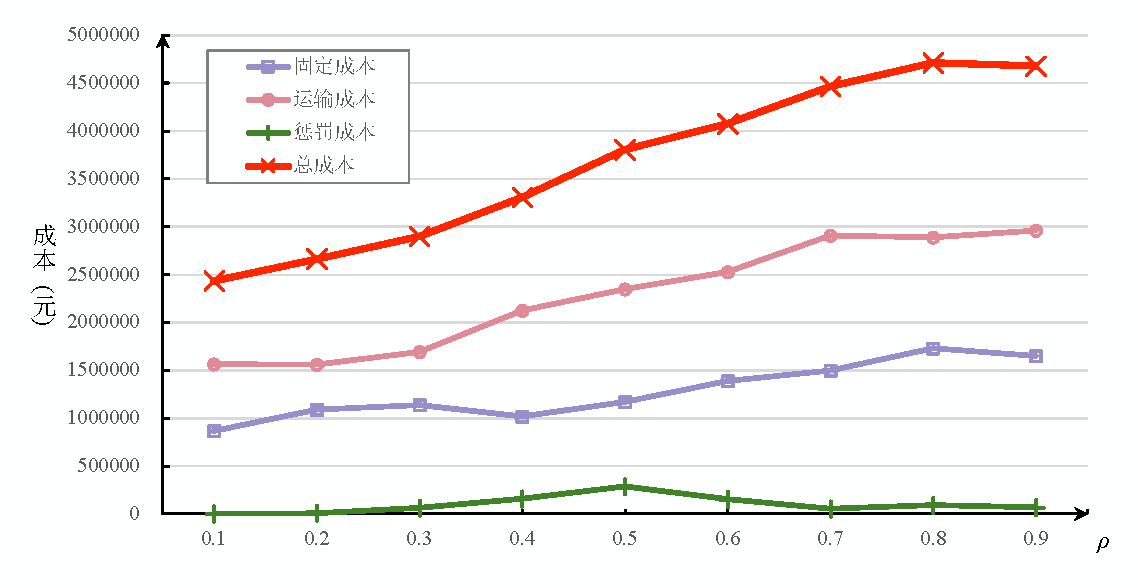
\includegraphics[width = 0.9 \textwidth]{figures/sens_rho.pdf}
	  \caption{成本随$\rho$变动的权衡曲线\\
	  Fig~\ref{fig:sens_rho}~ Trade-off curves for the variation of each cost with $\rho$}
	  \label{fig:sens_rho}
\end{figure}

\subsection{参数\texorpdfstring{$R$}{R}灵敏度分析}
本小节将分析参数$R$对选址结果的影响,
设置参数$\rho=0.1$,
参数$R$等于2至10的不同整数值,
即每个客户拥有0个至8个备用节点。
参数$R$控制每个客户拥有的常用节点、备用节点和虚拟节点的总数量。
已知每个客户必须拥有一个虚拟节点和一个常用节点,
则$R$的最小值为2。
表\ref{table:sens_r}展示了不同$R$取值下的选址方案和成本构成。



\begin{table}[htbp]
    \setlength{\abovecaptionskip}{-0.05cm} %调整图片caption与正文之间的间距,table同理。可自己调整。
    \setlength{\belowcaptionskip}{-0.2cm} 
    \centering
    \renewcommand\arraystretch{0.9}
    \caption{不同参数$R$取值的选址结果。
    \\Table~\ref{table:sens_r}~Results for different $R$.}
	\resizebox{\linewidth}{!}{
		\small{
			\begin{tabular}{clcccc}
				\toprule %[2pt]设置线宽 
				\multirow{2}[0]{*}{$R$} & \makecell[c]{\multirow{2}[0]{*}{选址方案}} & \multirow{2}[0]{*}{总成本} & \multirow{2}[0]{*}{固定成本} & \multicolumn{2}{c}{期望运输成本} \\
				\cmidrule{5-6}
					&       &       &       & 运输成本  & 惩罚成本 \\
				\midrule
				2&	8,13,54,66					&4670884.11	&1620000	&1984693.82	&1066190.29 \\
				3&	81,94,95,120,127,142,149,150			&2591989.01	&890000		&1510101.65	&191887.36\\
				4&	81,94,120,123,127,131,141,142,149,150		&2410503.11	&1000000	&1395715.25	&14787.86\\
				5&	81,94,120,123,127,131,141,142,149,150		&2397743.05	&1000000	&1396787.65	&955.40\\
				6&	79,81,94,120,123,127,131,138,141,142,150	&2398531.47	&1130000	&1268481.33	&50.14\\
				7&	81,94,120,123,127,131,138,141,142,150		&2402250.12	&1000000	&1402247.14	&2.98\\
				8&	81,94,120,123,127,131,141,142,149,150		&2396859.14	&1000000	&1396858.93	&0.21\\
				9&	81,94,120,123,127,131,141,142,149,150		&2396858.96	&1000000	&1396858.95	&0.01\\
				10&	81,94,120,123,127,131,141,142,149,150		&2396858.95	&1000000	&1396858.95	&0.00\\
				\bottomrule  
			\end{tabular}%
		}
	}
    \label{table:sens_r}
\end{table}%

首先分析选址方案的变化,
当$R=2$时,此时问题的退化成UFL问题,
此时选址的数量较少,但固定成本较高。
由于未向任何客户指派备用节点,因此$R=2$时方案的惩罚成本非常高。
当$R=3$时,即向每个客户指派1个备用节点,
惩罚成本大幅度下降。
这说明向客户即便向每个客户仅指派1个备用节点,
也能显著提高网络的可靠性。
随着每个客户备用节点数量的增加,
惩罚成本下降。
最终选址方案趋于稳定,总成本不再明显变化。
选址方案受参数$R$的影响较小,
结果鲁棒性较强,
表明在81、94、120、123、127、131、142、149、150等选址点处建设设施具有可靠性。

其次,相关成本随$R$的变化如图\ref{fig:sens_r}所示,
随着参数$R$的增加,
网络的总成本逐渐下降并趋于稳定。
产生该现象的原因是为每个客户安排常用节点,
降低了惩罚成本,
当惩罚成本几乎不变时,
选址结果同样不会变动。
图\ref{fig:sens_r}中展示的优化曲线表明为每个客户安排一个常用节点和三个备用节点时,
该网络已经变得足够可靠,
再向其添加备用节点对选址总成本不会产生较大的影响。

\begin{figure}[hbt] % use float package if you want it here
	%\setlength{\abovecaptionskip}{-0.2cm} %调整图片caption与正文之间的间距,table同理。可自己调整。
	\setlength{\belowcaptionskip}{-0.5cm} 
	  \centering
	  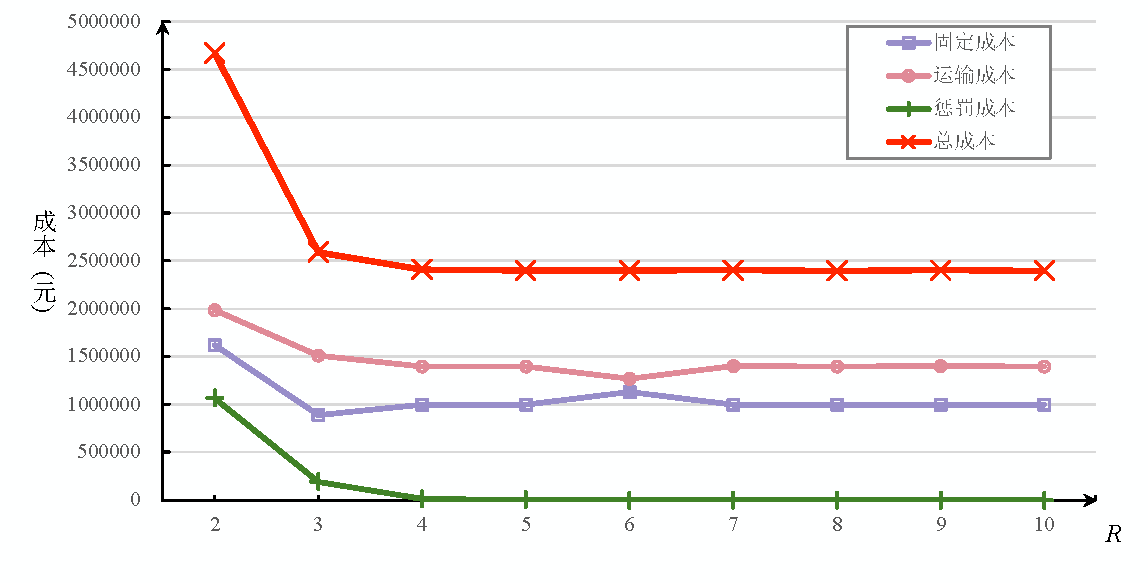
\includegraphics[width = 0.9 \textwidth]{figures/sens_r.pdf}
	  \caption{成本随$R$变动的权衡曲线\\
	  Fig~\ref{fig:sens_r}~ Trade-off curves for the variation of each cost with $R$}
	  \label{fig:sens_r}
\end{figure}

在本算例的灵敏度分析中,
系统的可靠性随备用节点个数的增加而增加。
然而,仅依靠增加备用节点个数以提高网络可靠性是有边界的。
超过此边界后,
再增加节点也很难影响选址方案和总成本。
在本算例中,$R=5$是每个客户拥有的最佳节点数量。
若$R$低于此值,网络变得不可靠,
若$R$高于此值,增加了运算量的同时对网络选址结果不产生较大影响。

\section{本章小结}
\label{sec:本章小结5}
本章的主要内容为数值实验和算例分析。
首先采用经典选址数据集构造了数值实验的算例,
对比分析了LR-ILS算法与商业求解器的求解结果。
结果表明,
根据问题定制的LR-ILS算法可以在短时间内获得近似最优解,
并且可以求解150个客户与150个候选位置的大规模数据。
在绝大多数算例中,
LR-ILS求解结果和求解时间显著优于求解器。
此外,数值实验还针对LR-ILS算法的各种算子性能和算法设计展开了分析,
特别是求解模型上界、下界的性能,
以及多种乘子初始化和更新方法的效果。
数值实验还讨论了模型线性化的效果,
对比分析使用求解器求解非线性模型和线性模型的差异。
最后,给出了算例选址结果,以及重要参数的灵敏度分析结果。
值得注意的是,
由于该算法使用了元启发式算子,
算法本质上带有随机性,
因此会造成运行最终结果中上界不稳定的情况。
但是,算法的下界提供了上界质量的证明。

                % 第五章
 \setlength{\baselineskip}{20pt}
\chapter{总结与展望}
\label{cha:summary}

本章的\ref{sec:summary}节总结本文工作内容,
并指出了本文可完善的部分,
为后续工作指明改进方向,
此外,
第\ref{sec:future}节还展望了有关可靠选址问题的未来研究方向,
提出了当前研究的热点和未来有意义的研究内容。

% TODO 拉格朗日松弛-迭代局部搜索算法 

\section{工作总结}
\label{sec:summary}
本文研究了物流节点可靠选址及客户分配模型与算法,
研究的主要内容为模型和算法。
考虑到物流节点在现实运营中将面临一系列可能导致其失效的风险因素,
以及节点失效时客户的行为,
本文构建了考虑节点失效风险的物流网络选址模型,
并设计了基于迭代局部搜索改进的拉格朗日松弛算法。
数值实验结果展示了算法可求解大规模算例的优越性能。
最后,本文进行物流节点可靠选址算例计算,
为物流节点选址提供了理论支撑。
论文的主要研究内容总结和结论如下:

\begin{enumerate}[label=(\arabic*),leftmargin=0pt,itemindent=3.5\ccwd, nosep]
    \item 基于可靠选址理论,考虑到客户的不完全信息状态,
    本文描述了客户的试错过程,
    构建了节点端提供服务的物流节点可靠选址问题,
    该问题被证明为NP-hard问题。
    本文的问题可构建为非线性整数规划模型,
    使用线性化技术消除模型中的非线性成分。
    此外,本文提出了一个与该问题相关的最短路问题,
    并给出了该问题的数学模型。
    
    \item 本文定制了基于迭代局部搜索改进的拉格朗日松弛算法,
    启发式算子快速获得模型的上下界的近似值,
    深度优先搜索算法再对上下界结果进行改进,得到上下界的精确值。
    迭代局部搜索算子对拉格朗日松弛上界选址方案进行局部搜索以进一步提升上界质量。

    \item 本文对比了基于迭代局部搜索改进的拉格朗日松弛算法和求解器的性能,
    实验结果表明基于迭代局部搜索改进的拉格朗日松弛算法具有求解大规模问题和现实案例的能力。
    本文详细讨论了算法每个算子的效果,
    通过数值实验对比了算子的效率,
    虽然深度优先搜索算子是非多项式时间算法,
    但在求解该问题时仍展现了良好的效果。
    
    \item 本文进行了灵敏度分析,
    结果表明:
    每个客户拥有一个常用节点和两个备用节点即可提升网络的可靠性。
    在一定范围内,
    随着运价和失效概率的提升,
    系统的总成本提升但能保持选址方案不变。
    当运价和失效概率的提升超过一定幅度,
    增加节点建设数量是降低系统成本、维持系统可靠性的方法之一。
    
\end{enumerate}

限于作者的自身理论水平以及代码编写水平,
本文的研究内容也有一系列的局限性。
模型方面,本文描述了客户常用节点失效后的试错以寻找设施的行为,
绝对的不完全信息场景和绝对的完全信息场景都是假设前提,
但现实中的情况远远比实际情况复杂,
很可能是不完全信息场景和完全信息场景的混合。
此外,模型假设每个节点的失效是彼此独立的,
该假设主动忽视了节点之间的联系。
算法方面,虽然拉格朗日松弛算法能提供一个相对较紧的下界,
但对于大规模的问题,
该算法的效果同样有限。
并且,拉格朗日松弛算法在大多数情况下只能得到一个近似最优解。
此外,算法的算子为非多项式时间算法,
对于一些特殊且复杂的问题,
在最差的情况下无法保证求解时间。
最后,受限于作者编写代码水平和Matlab解释型语言的性能,
当前算法仍有进一步改进的空间。


\section{研究展望}
\label{sec:future}

针对当前研究的局限性,
未来研究的可改进之处以及研究方向如下:

\begin{enumerate}[label=(\arabic*),leftmargin=0pt,itemindent=3.5\ccwd,listparindent = 2\ccwd, nosep]
    \item 现有模型考虑因素的改进。
    
    未来研究可对当前的模型考虑的不完全信息场景进一步改进,
    可混合完全信息和不完全信息场景,
    使得模型更加贴近现实。
    此外,现实中风险可导致多个节点同时失效,
    模型的节点失效独立性假设也可进一步改进。
    如何构建节点之间的失效关联方程,
    特别是离散选址模型中该方程的定义,
    是未来研究的重点。
    对于当前研究的可靠选址问题,
    未来的研究中还可将其应用至更多场景中,
    例如可靠基础设施选址(电动车充电站、零售企业选址)等,
    还可与其他经典选址问题融合,
    构建可靠选址-路径问题、可靠选址-库存问题、多周期可靠选址问题等。

    \item 现有算法的改进。
    
    在本文原模型的上界和下界的求解过程中,
    都不可避免地反复求解一个最短路问题。
    该最短路问题考虑了每个节点的失效可能,
    具有一定的特殊性,
    使得经典求解最短路问题的算法失效。
    但是,在该最短路问题中,
    所有弧的权重为正值,
    利用该特性可以降低求解该问题的复杂性。
    由于该问题同样为NP-hard问题,
    因此求解该问题的不存在多项式时间算法,
    但可能存在伪多项式时间算法。
    可考虑将脉冲算法、标签算法移植到本问题中,
    推动求解原问题的进程,
    使得算法更具有效率。

    \item 求解模型的其他算法。
    
    使用拉格朗日松弛算法得到结果不能保证其最优性,
    但可获得解的下界。
    利用本文中构建迭代局部搜索算子的思路,
    可以开发出元启发式算法。
    但元启发式算法只能给出一个可行解,
    并不能证明解的质量。
    所以,未来研究的另一个方向是开发求解模型的精确算法。
    Benders分解是一种求解混合整数规划问题、选址问题常用的精确算法。
    开发求解本问题的Benders分解算法,
    是未来研究中有深度的算法创新。

\end{enumerate}
                % 第七章
 
\nocite{*}
\bibliography{reference/ref}                % 参考文献

\backmatter
\setlength{\baselineskip}{16pt}
\chapter{附录A}
\label{cha:app1}
%\section*{附录标题}
%\zihao{5}
%[内容为五号宋体。] 附录是作为论文主体的补充项目,并不是必须的。
%论文的附录依序用大写正体英文字母A、B、C……编序号,如:附录A。
%\vspace{0.75cm}
\begin{center}
\zihao{3}
\textbf{ILS-LR算法源码}
\end{center}

\indent
\zihao{-4}
该代码包含算法的主程序及所有函数,
算法所需的数据请见正文中的参考文献。
此外,作者的Github开源仓库\footnote{https:\slash \slash github.com\slash yrf990409\slash LR\_for\_RUFL}
提供了同样的代码、数据以及环境配置方法,
以方便感兴趣的读者复现。
本附录的第一部分是LR-ILS算法的Matlab算法,
第二部分是Gurobi建模Python代码。

\subsection*{LR-ILS算法源码(Matlab)}
\vspace{-20pt}
\small{
    \begin{lstlisting}[language=Matlab,
        breaklines=true, % 自动换行
        frame = leftline,
        linewidth = \textwidth,
        texcl = false,
        columns=flexible,
        lineskip=1pt,
        keywordstyle=\color{blue!90}\bfseries, %代码关键字的颜色为蓝色,粗体
        numbers=left,%左侧显示行号
        numberstyle=\small, %行号字体用小号
        showspaces=false, %
        fontadjust,
        basicstyle = \fontspec{Times New Roman},
        basicstyle = \songti
        ]
    % 拉格朗日松弛求解可靠设施选址问题(RUFL)
    % 编码方式: UTF-8
    % 操作系统: Windows 10/11 & MacOs 13
    % 运行平台:
    % Matlab R2022a/b 
    % 工具箱 Matlab Coder & Parallel Computing
    % Gurobi 9.5.2
    % Python 3.10

    % 清除
    clc
    clear all
    clear classes
    close all 
    diary off
    diary 'LR.log'
    disp(['程序开始: ', datestr(now)])

    %% 参数控制
    lr_para = struct();             % LR 算法的参数
    lr_para.alpha       = 2;        % 步长参数初始值
    lr_para.alpha_min   = 0.0001;   % 步长参数最小值
    lr_para.theta_lr    = 1.05;      % 步长比例系数
    lr_para.kappa_lb    = 10;       % 下界连续不变次数
    lr_para.eta_lr      = 3000;     % 迭代次数
    lr_para.tau_lim     = 1000;     % 优化时长
    lr_para.xi          = 0.01;     % 接受gap
    lr_para.theta_sa    = 1.2;      % 模拟退火初始温度参数
    lr_para.T_lim       = 0.0001;   % 模拟退火最低温度
    lr_para.kappa_ub    = 100;      % 触发ILS上界连续不变次数 (200)
    lr_para.kappa_ubdfs = 500;      % 触发上界DFS搜索(delete)
    lr_para.eta_ils     = 10;       % ILS迭代次数
    lr_para.grb_model   = 1;        % 使用Gurobi建模 取值 0 1
    lr_para.grb_ub      = 1;        % 使用Gurobi获取上界 取值0 1
    lr_para.dfs_gap     = 0.2;      % gap小于此值才启动DFS
    lr_para.print       = true;     % 解池的大小

    %% 案例参数
    % lr_case = struct();
    % path = './data/SnyderData/49nodes/';
    lr_case.data = data_reader(path);
    lr_case.rho = prob_rho;                                     % 损坏概率控制参数
    lr_case.q = lr_case.rho * exp(-lr_case.data.fix/200000);    % 损坏概率
    lr_case.q(1) = 1;                                           % 虚拟设施的损坏概率
    lr_case.max_try = out_index;                                % 最大尝试次数(R)
    lr_case.cus_num = length(lr_case.data.dmd);                 % 客户数量
    lr_case.node_num = size(lr_case.data.price,1);              % (虚拟 实体 客户)的总数
    lr_case.fac_num = lr_case.node_num - lr_case.cus_num - 1;   % 设施总数
    lr_case.bar_J = (0:lr_case.fac_num)+1;                      % 设施集合拓展集
    lr_case.I = (lr_case.fac_num+1 : lr_case.node_num-1)+1;     % 客户集合
    lr_case.mu = zeros(lr_case.cus_num, length(lr_case.bar_J)); % 生成初始乘子
    for i = 1:lr_case.cus_num
        cus_ind = lr_case.I(i)-lr_case.I(1)+1;
        for j = lr_case.bar_J(2:end)
            lr_case.mu(:,j) = (lr_case.data.dmd(cus_ind) * lr_case.data.price(cus_ind,j) + ...
                lr_case.data.fix(j)) / length(lr_case.data.fix);
        end
    end

    %% 优化
    lr_result = lr_ils(lr_para, lr_case);

    %% 结果处理
    % draw_fig(lr_result)

    % 保存
    file_name = ['结果', ...
                num2str(lr_case.node_num), '-' , ... % 点数
                num2str(lr_case.rho),      '-' , ... % rho取值
                num2str(lr_case.max_try),  '-' , ... % 最大试错次数
                '.mat'];
    save(file_name,'lr_result')

    % fprintf('rho \t 最大试错次数 \t 上界 \t 下界 \t 求解时间\text{\\n}')
    fprintf('%d \t %.2f \t %d \t %.2f \t %.2f \t %.2f \n', lr_case.node_num, lr_case.rho, lr_case.max_try, lr_result.bst_ub, lr_result.bst_lb, lr_result.time)
    diary off

    function data = data_reader(f_path)
    %DATA_READER 读取数据
    %   data包含三个数据
    %% 数据读取
    % disp(['导入数据,当前路径: ', f_path])
    data.price = load([f_path, 'cost.csv']); % 价格矩阵
    data.dmd = load([f_path, 'dmd.csv']);    % 客户需求
    data.fix = load([f_path, 'fc.csv']);     % 固定成本
    % disp('导入完成!')
    % disp('---------------------------------')

    % 验证数据
    validateattributes(data.price, {'double'}, {'size', [length(data.dmd)+length(data.fix), length(data.fix)]})

    end

    function [ub,best_r] = lb_dfs(r, best_r, ub, cur_cost, cur_prob, fac, cus_dmd, ...
        cost_mat, R, pi, probDisr, cus_mu)
    % global x
    % x = x+1
    if length(r) <= R+1 % 没有到达设施数量的上界
        if r(end) == 1 % 如果结尾是虚拟,那么获得了一个完整路径
            tempCost = cur_cost;
            if tempCost < ub % 小于上界 则更新
                ub = tempCost;
                best_r = r;
                return
            end
            return
        else % 否则不是一个完整路径
            if isempty(fac) % 没有设施可以填充了,route最后一个不以虚拟结尾
                r = [r,1]; % route必须是虚拟收尾了

                tempCost = cur_cost + cus_dmd*pi*cur_prob;
                if tempCost < ub % 小于上界 则更新
                    ub = tempCost;
                    best_r = r;
                    return
                end
                return
            else % 还有设施可以填充
                if length(r) == R+1 % 已经填满,放不下了,只差一个虚拟设施
                    r = [r,1]; % route必须是0收尾了
                    tempCost = cur_cost + cus_dmd*pi*cur_prob;
                    if tempCost < ub % 小于上界 则更新
                        ub = tempCost;
                        best_r = r;
                        return
                    end
                    return
                else % 向下继续分支
                    for i = 1:length(fac) % i : index of facilities
                        stackR = r;
                        stackC = cur_cost;
                        stackP = cur_prob;

                        r = [r,fac(i)];
                        tempCost = cur_cost + cost_mat(r(end-1),r(end))*cur_prob*cus_dmd + cus_mu(1,fac(i));

                        if tempCost>ub % 剪枝
                            r = stackR; % 直接恢复不再细分
                        else
                            tempFacy = fac;  % 递归 继续分支
                            tempFacy(tempFacy==fac(i)) = [];
                            cur_prob = cur_prob*probDisr(r(end));
                            [ub,best_r] = lb_dfs(r,best_r,ub,tempCost,cur_prob,tempFacy,cus_dmd,cost_mat,R,pi,probDisr,cus_mu);
                            r = stackR;
                            cur_cost = stackC;
                            cur_prob = stackP;
                        end
                    end
                end
            end
        end
    else
        return
    end
    end
    
    function [trans_cost, plan] = lb_x(lr_case, flag_fast)
    %lb_dfs_x 深度搜索获取每个客户的尝试路径

    % 输入 lr_case 字段
    % I         客户索引 向量
    % bar_J     设施索引 向量
    % data      数据 结构体 字段 price价格矩阵 dmd客户需求 fix固定成本
    % q         每个设施失效概率 向量
    % mu        拉格朗日乘子 矩阵
    % max_try   客户最大尝试次数 整数
    % dfs_falg  是否使用DFS 逻辑值

    % 输出
    % trans_cost    期望运输成本   浮点数矩阵
    % plan          计划          整数矩阵

    %% 初始化
    % 提取
    I = lr_case.I;
    bar_J = lr_case.bar_J;
    data = lr_case.data;
    q = lr_case.q;
    mu = lr_case.mu;
    max_try = lr_case.max_try;
    trans_cost = zeros(length(I),1);    % 记录每个客户的期望运输成本

    %% 贪心路径构建
    [plan, trans_cost] = greedy_build(I, max_try, bar_J, data, mu, q, trans_cost);

    %% DFS改进当前解
    if ~flag_fast % 快速模式不启动dfs
        dmd = data.dmd;
        price = data.price;
        pi = price(2,1);    % 惩罚成本
        parfor j = 1:length(I)
            cus = I(j);
            best_r = plan(j,:); % 当前最优路径
            ub = trans_cost(j); % 当前上界
            cus_dmd = dmd(j); % 客户的需求
            cus_mu = mu(j,:);  % 拉格朗日乘子

            R = coder.ignoreConst(max_try-1);
            coder.varsize('cus', [1 100], [0 1]);
            coder.varsize('best_r');
            coder.varsize('bar_J');
            coder.varsize('price');
            coder.varsize('q');
            coder.varsize('cus_mu');

            [ub, best_r] = lb_dfs(cus, best_r, ub, 0, 1, bar_J, cus_dmd, price, R, pi, q, cus_mu); % 深度优先搜索
            trans_cost(j) = ub; % 更新上界

            if length(best_r) < max_try+1
                plan(j,:) = [best_r, zeros(1, max_try+1-length(best_r))];
            else
                plan(j,:) = best_r; % 记录方案
            end

        end
    end
    end


    function [plan, trans_cost] = greedy_build(I, max_try, bar_J, data, mu, q, trans_cost)
    % 路线构建的贪心算法
    % 在每个路径的最后增加一个算子
    plan = zeros(length(I), max_try+1); % 记录每个客户的方案
    dmd = data.dmd; % 客户的需求
    price = data.price; % 价格矩阵
    for k = 1:length(I)
        cus = I(k);
        % 直接采用构造法生成一个初始路径
        route = zeros(1, max_try+1); % 路径
        route(1) = cus; % 路径的起点是客户
        prob = 1;   % 初始概率是1
        fee = 0;    % 初始费用是0
        fac = bar_J;    % 设施的复制
        cus_dmd = dmd(k); % 客户的需求
        jdg_brk = false;
        
        mu_k = mu(k,:);
        % 每次讲增量成本最小的设施放在路线最后(贪心构建)
        for i = 2:max_try
            add_fee = zeros(1,length(fac));
            for j = 1:length(fac)
                add_fee(j) = prob * cus_dmd * price(route(i-1),fac(j)) ...
                    + mu_k(fac(j));
            end
            [min_add_fee,min_ind] = min(add_fee); % 指向最小的费用
            route(i) = fac(min_ind); % 路线更新
            prob = prob * q(route(i)); % 概率更新
            fee = fee + min_add_fee; % 费用更新
            if route(i) == bar_J(1)
                jdg_brk = true;
                break % 如果虚拟设施被添加到路径中则退出
            end
            fac(min_ind) = []; % 否则去除已经添加的设施
        end

        if jdg_brk % 提前退出
            plan(k,:) = route; % 记录路径
            trans_cost(k) = fee; % 记录成本
        else
            route(route==0) = []; % 去除路径中的多余0
            trans_cost(k) = fee + cus_dmd * prob * price(route(end),1); % 直接计算成本

            formated_route = [route, 1, zeros(1, max_try-length(route))]; % 记录路径
            plan(k,:) = formated_route; % 记录路径
        end
    end
    end


    function [cost_for_fac, location] = lb_y(lr_case)
    %LB_Y获取y变量的下界
    % 给定一个乘子,返回y的最佳选址location以及设施建设成本cost_for_fac

    % 初始化
    bar_J = lr_case.bar_J;
    data = lr_case.data;
    mu = lr_case.mu;

    location = false(1,length(bar_J));     % 选址方案
    cost_for_fac = zeros(1,length(bar_J)); % 下界Sub_1问题的目标函数

    for j = 2:length(bar_J)
        fac = bar_J(j);
        sum_mu = sum(mu(:,fac)); 
        jdg = data.fix(fac) - sum_mu; % 判别

        if jdg > 0 % 判别数大于0 不选这个位置
            location(fac) = 0;
        else
            location(fac) = 1; % 小于等于0 选
            cost_for_fac(fac) = data.fix(fac) - sum_mu;
        end

    end

    end

    function lr_result = lr_ils(lr_para, lr_case)
    % LR_ILS 拉格朗日松弛-局部迭代搜索算法
    % 传入 案例参数lr_case 以及算法参数lr_para
    % 传出 lr_result结果

    %% 初始化
    tic
    % 记录 recorder
    rec_lb  = zeros(lr_para.eta_lr, 1);     % 下界记录 record
    rec_ub  = zeros(lr_para.eta_lr, 1);     % 上界记录
    rec_ils = false(lr_para.eta_lr, 1);     % ILS发挥作用记录

    % 计数器 count
    cnt_step = 0;   % 下界连续不上升计数
    cnt_ils  = 0;   % 上界连续不下降计数
    cnt_ub   = 0;   % 最佳上界保持的迭代次数
    cnt_iter = lr_para.eta_lr;  % 算法真正的迭代次数

    % 最佳解 best_solution
    bst_loc  = false(1, length(lr_case.bar_J));             % 最佳选址方案 location
    bst_sqc  = zeros(length(lr_case.I), lr_case.max_try+1); % 最佳客户序列 sequence
    bst_ub   = inf;     % 最佳上界
    bst_lb   = -inf;    % 最佳下界
    gap = 1;

    % 条件判断 flag
    flag_fast = true;       % 算法快速模式
    flag_modify = false;    % 快速\&慢速切换时强制更正上下界
    flag_ils_continue = false;  % ILS是否继承上一次的结果

    % 邻域
    cur_ub = inf;
    cur_loc = false(1,length(lr_case.bar_J));     % 选址方案

    %% LR-ILS优化
    for iter = 1:lr_para.eta_lr
        % 获取下界
        [lb_val_x, lb_sqc] = lb_x(lr_case, flag_fast);  % 获取Sub_2的值
        [lb_val_y, lb_loc] = lb_y(lr_case);             % 获取Sub_1的值
        lb = sum(lb_val_x) + sum(lb_val_y);

        % 获取上界
        [ub, sqc, ~] = ub_xy(lr_case, lb_loc, flag_fast);

        % ILS搜索上界
        if cnt_ub >= lr_para.kappa_ub && gap > 2*lr_para.xi
            if flag_ils_continue
                [nb_ub, nb_loc, cur_ub, cur_loc] = ub_ils(lr_case, cur_ub, cur_loc, lr_para);
            else
                [nb_ub, nb_loc, cur_ub, cur_loc] = ub_ils(lr_case, bst_ub, bst_loc, lr_para);
            end

            if nb_ub < bst_ub
                % 得到更好的上界
                bst_loc  = nb_loc;  % 选址方案
                bst_ub   = nb_ub;   % 上界 
                rec_ils(iter) = true;
            else
                flag_ils_continue = true;  % ILS继承上一次的结果
            end

            cnt_ub = 0;
        end

        % 记录最佳上界
        if ub <= bst_ub
            % 得到了更好的上界
            bst_loc  = lb_loc;  % 选址方案
            bst_sqc  = sqc;     % 客户序列
            bst_ub   = ub;      % 上界
            % 计数器更新
            cnt_ils = 0;        % 上界连续不下降
            cnt_ub  = 0;        % 最佳上界保持次数
            % 局部迭代搜索更新

        else
            % 计数器更新
            cnt_ils = cnt_ils + 1; % 上界连续不下降
            cnt_ub  = cnt_ub + 1;  % 最佳上界保持次数
        end

        % 记录最佳下界
        if lb >= bst_lb
            bst_lb = lb;
            cnt_step = 0;
        else
            cnt_step = cnt_step + 1; % 否则下界未更新计数+1
        end

        % 更新乘子
        [lr_case.mu, cnt_step, lr_para.alpha] = update_mu(lr_case, lr_para, lb, bst_ub, lb_sqc, lb_loc, cnt_step);

        % 迭代记录
        rec_lb(iter)  = lb;         % 下界记录 record
        rec_ub(iter)  = bst_ub;     % 上界记录
        

        % 打印
        gap = (bst_ub-bst_lb) / bst_ub; % 计算gap
        t = toc;
        if lr_para.print
            formatSpec = "iter:%.0f, best-ub:%.2f, best-lb:%.2f, gap:%.4f%%, time:%.2f, ub:%.2f, lb:%.2f\n";
            fprintf(formatSpec, iter, bst_ub, bst_lb, gap*100, t, ub, lb);
        end
        

        % 快速慢速切换
        if gap <= lr_para.dfs_gap && ~flag_modify % gap小于一定的值 关闭快速模式
            flag_fast = false;  % 关闭快速模式
            flag_modify = true; % 强制修正
            % 快速模式获得的下界不是最优解,因此下界是虚标的,在此处进行修正
            [lb_val_x, ~] = lb_x(lr_case, flag_fast);  % 获取Sub_2的值
            [lb_val_y, ~] = lb_y(lr_case);             % 获取Sub_1的值
            bst_lb = sum(lb_val_x) + sum(lb_val_y);    % 强制修正下界
            gap = (bst_ub-bst_lb) / bst_ub;            % 修正之后的gap
        end

        % 终止条件
        if t > lr_para.tau_lim
            disp('stop, time') % 时间限制
            cnt_iter = iter;
            break
        else
            if lr_para.alpha < lr_para.alpha_min
                disp('stop, alpha') % 迭代值限制
                cnt_iter = iter;
                break
            elseif gap < lr_para.xi
                disp('stop, gap') % gap值达标
                cnt_iter = iter;
                break
            end
        end
    end
    if cnt_iter == lr_para.eta_lr
        disp('stop, iteration') % 迭代次数限制
    end

    %% 封装 & 返回      
    % 重新计算
    t = toc;
    lr_result         = struct();
    lr_result.rec_lb  = rec_lb;
    lr_result.rec_ub  = rec_ub;
    lr_result.rec_ils = rec_ils;
    lr_result.bst_loc = bst_loc;
    lr_result.bst_sqc = bst_sqc;
    lr_result.bst_ub  = bst_ub;
    lr_result.bst_lb  = bst_lb;
    lr_result.iter    = cnt_iter;
    lr_result.time    = t;


    end

    function [best_nb_ub, best_nb_loc, current_ub, current_loc] = ub_ils(lr_case, ub, location, lr_para)
    %UB_ILS 局部迭代搜索
    %% 初始化
    best_nb_ub = ub;                 % 记录全局最佳上界
    best_nb_loc = location;          % 记录全局最佳选址方案

    current_ub = ub;            % 当前上界
    current_loc = location;     % 当前方案

    temperature = -(lr_para.theta_sa-1)*ub/log(0.5);  % 初始温度
    t_gap = temperature / (lr_para.eta_ils*0.4);      % 每次降低的温度

    for iter = 1:lr_para.eta_ils
        % 求邻域
        nb = get_nb(current_loc); % 获取邻域
        nb_sz = size(nb,1);

        % 求所有邻域中成本最小的几个
        nb_cost_rec = zeros(nb_sz,1);
        for i = 1:size(nb,1)
            [nb_cost_rec(i), ~] = ub_xy(lr_case, nb(i,:), true); % 求快速解
        end
        [~, sort_ind] = sort(nb_cost_rec);    % 最小成本索引

        % 计算前 5 个 最佳索引的精准上界
        temp_best_loc = nb(sort_ind(1:5),:);
        temp_cost_rec = zeros(5,1);
        for i = 1:5
            [temp_cost_rec(i), ~] = ub_xy(lr_case, temp_best_loc(i,:), false); % 求快速解
        end
        
        [best_nb_cost, min_ind] = min(temp_cost_rec);

        % 接受上界
        if best_nb_cost < current_ub    % 得到更优质的解
            current_ub = best_nb_cost;              % 记录临时上界
            current_loc = temp_best_loc(min_ind,:); % 临时选址方案
        else % 概率接受不那么好的解
            if rand < exp((best_nb_cost - current_ub )/temperature)
                current_ub = best_nb_cost;          % 记录临时上界
                current_loc = nb(i,:);          % 临时选址方案
            end
        end
        
        % 更新最优解
        if current_ub < best_nb_ub % 获得全局最优解直接返回
            best_nb_ub = current_ub;             % 记录全局最佳上界
            best_nb_loc = current_loc;           % 记录全局最佳选址方案
        end
        
        % 更新温度
        temperature = temperature - t_gap;
        if temperature <= 0
            temperature = 0.0001;
        end
    end

    end

    function ns = get_nb(location)
    location(1) = []; % 先删除虚拟设施
    opened = find(location == 1);
    closed = find(location == 0);

    % 计算需要邻域的大小
    ns_sz = length(opened) + length(closed) + length(opened) * length(closed);
    ns = false(ns_sz,length(location));

    count = 1;
    % 关闭一个设施
    for i = 1:length(opened)
        temp = location;
        temp(opened(i)) = 0;
        ns(count,:) = temp;
        count = count + 1;
    end

    % 开启一个设施
    for i = 1:length(closed)
        temp = location;
        temp(closed(i)) = 1;
        ns(count,:) = temp;
        count = count + 1;
    end

    % 交换设施状态
    for i = 1:length(opened)
        for j = 1:length(closed)
            temp = location;
            temp(opened(i)) = 0;
            temp(closed(j)) = 1;
            ns(count,:) = temp;
            count = count + 1;
        end
    end

    % 补充虚拟设施
    ns = [true(size(ns,1),1) ns];
    end


    function [mu, cnt_step, alpha] = update_mu(lr_case, lr_para, lb, ub, plan_lb, location, cnt_step)
    %乘子更新

    % 提取
    I = lr_case.I;
    bar_J = lr_case.bar_J;
    mu = lr_case.mu;
    alpha = lr_para.alpha;

    % 更新系数
    if cnt_step > lr_para.kappa_lb % 长时间未更新下界则步长因子打折
        alpha = alpha / lr_para.theta_lr; % 步长系数打折
        cnt_step = 0; % 打折后计数器归零
    end

    temp = zeros(length(I), length(bar_J)); %记录客户i是否使用了设施j
    % 计算分母
    for i = 1:size(plan_lb,1)
        fac_use = plan_lb(i, 2:end); % 对于i来说使用了的设施
        fac_use(fac_use==0) = [];
        temp(i, fac_use) = 1;
    end
    violate = temp - location; % 违背约束

    % 计算迭代步长
    k_step = lr_para.alpha * (ub-lb) / sum(abs(violate),"all");

    % 更新乘子
    for m =2:length(bar_J)
        j = bar_J(m);   % j 是设施
        if location(j)
            y_j = 1;
        else
            y_j = 0;
        end

        for n = 1:length(I)
            i = I(n) - bar_J(end); % i 是客户
            if any(plan_lb(i,2:end) == j)
                x_ikj = 1;
            else
                x_ikj = 0;
            end
            mu(i, j) = mu(i, j) + k_step * (x_ikj - y_j);
            if mu(i,j) < 0
                mu(i,j) = 0;
            end
        end
    end


    function [obj, plan, trans_cost] = ub_xy(lr_case, location, flag_fast)
    %UB_YX求解模型的上界
    % OBJ 返回原问题的最优目标函数
    % plan 返回最优路径方案
    % trans_cost 返回各路径的运输成本

    %% 初始化
    % 提取
    I = lr_case.I;
    bar_J = lr_case.bar_J;
    data = lr_case.data;
    q = lr_case.q;
    max_try = lr_case.max_try;
    dmd = data.dmd;
    price = data.price;

    trans_cost = zeros(length(I),1);    % 记录每个客户的期望运输成本
    fix_cost = data.fix(location);      % 计算固定成本
    plan = zeros(length(I), max_try+1); % 记录每个客户的方案
    location(1) = 1;                    % 虚拟设施指定是已经建设的
    q_loc = q(location);                % 已建设施的损坏概率
    located = find(location==1);        % 已经建设的设施的索引

    price_located = price(location,:);  % 建设的节点之间的价格
    price_cus_fac = price(length(bar_J)+1:end,:); % 顾客和建设的节点之间的距离
    parfor i = 1:length(I)
        cus = I(i);
        % 初始化客户相关变量
        
        dmd_cus = dmd(i); % 节点需求
        price_cus = [price_located; 
                    price_cus_fac(i,:)]; % 价格矩阵去掉多余行
        price_cus = price_cus(:,location);  % 价格矩阵去掉多余列

        % dijkstra
        [pind_without_cus, trans_cost_cus] = mod_dijkstra(price_cus, q_loc, dmd_cus, max_try);
        
        % 记录
        trans_cost(i) = trans_cost_cus;
        temp = [cus, pind_without_cus];

        if length(temp) < max_try+1
            plan(i,:) = [temp, zeros(1, max_try+1-length(temp))];
        else
            plan(i,:) = temp; % 记录方案
        end
    end

    for i = 1:size(plan,1)
        pind_with_cus = plan(i,:);
        pind_with_cus(pind_with_cus==0) = [];
        temp = [pind_with_cus(1), located(pind_with_cus(2:end))];
        if length(temp) < max_try+1
            plan(i,:) = [temp, zeros(1, max_try+1-length(temp))];
        else
            plan(i,:) = temp; % 记录方案
        end
    end

    obj = sum(trans_cost) + sum(fix_cost); % 目标函数值

    if ~flag_fast
        % 快速模式不启动dfs
        [obj, plan, trans_cost] = ub_dfs(I, bar_J, location, plan, trans_cost, data, q, max_try);
    end

    end


    function [pind_without_cus, trans_cost] = mod_dijkstra(price, q_loc, dmd_cus, max_try)
    %MOD_DIJKSTRA 修正的Dijkstra算法
    % 输入一个i行j列的距离矩阵(从i到j),返回从最后一个点到第一个点最短成本的路径
    % 传入的距离矩阵最后一行表示客户,第一行是虚拟设施

    start = size(price,1);  % 初始起点
    fee = 0;                % 当前产生的费用
    preceding_ind = zeros(1, length(q_loc));   % 前向记录
    prob = ones(1, length(q_loc)+1);           % 概率记录
    unmark = 1:length(q_loc);                  % 未标记的点
    weight = inf * ones(1, length(q_loc));     % 点的权重

    count = 0;
    while count < max_try
        % 更新未扫描的节点
        for j = 1:length(unmark)
            % 上一个点产生的费用 加上 到这个点需要的费用
            temp = fee + prob(start) * dmd_cus * price(start, unmark(j));

            if temp < weight(unmark(j)) % 得到新的权重
                weight(unmark(j)) = temp;
                preceding_ind(unmark(j)) = start; 
            end
        end

        [fee, mind_unmark] = min(weight(unmark));   % 在所有未标记的权重中选取最小
        start = unmark(mind_unmark);                % 更新起点
        unmark(unmark==start) = [];                 % 更新标记
        prob(start) = prob(preceding_ind(start)) * q_loc(start);   % 更新概率
        
        if start == 1
            break
        end
        if isempty(unmark)
            break
        end
        count = count + 1;
    end

    trans_cost = weight(1);
    pind_without_cus = get_plan(preceding_ind, max_try, 1, size(price,1));

    end

    function plan_without_cus = get_plan(preceding, times, p_start, p_end)
    % 返回一个不带客户的路线方案
    % 给定DIJKSTRA算法的跟踪索引,返回一个路径
    plan_without_cus = zeros(1, times);
    ind = p_start;
    plan_without_cus(1) = ind;

    count = 2;
    while 1
        if preceding(ind) == p_end
            break
        end

        plan_without_cus(count) = preceding(ind);
        ind = preceding(ind);

        count = count+1;
    end
    plan_without_cus = plan_without_cus(end:-1:1); % 逆转
    plan_without_cus(plan_without_cus==0) = [];    % 除0
    end

    function [lr_ub, plan, trans_cost] = ub_dfs(I, bar_J, location, plan, trans_cost, data, q, max_try)
    %UB_DFS 上界DFS搜索
    pi = data.price(2,1);    % 惩罚成本
    cus_mu = zeros(1,length(bar_J)); % 上界没有乘子
    dmd = data.dmd;
    price = data.price;
    parfor j = 1:length(I)
        cus = I(j);
        best_r = plan(j,:); % 当前最优路径

        ub = trans_cost(j); % 当前上界
        cus_dmd = dmd(j); % 客户的需求
        
        fac = find(location==1); % 已经建设的设施

        R = coder.ignoreConst(max_try-1);
        coder.varsize('cus', [1 100], [0 1]);
        coder.varsize('best_r');
        coder.varsize('bar_J');
        coder.varsize('price');
        coder.varsize('q');
        coder.varsize('cus_mu');

        [ub, best_r] = lb_dfs(cus, best_r, ub, 0, 1, fac, cus_dmd, price, R, pi, q, cus_mu); % 深度优先搜索
        trans_cost(j) = ub; % 更新上界
        plan(j,:) = 0;
        if length(best_r) < max_try+1
            plan(j,:) = [best_r, zeros(1, max_try+1-length(best_r))];
        else
            plan(j,:) = best_r; % 记录方案
        end
    end

    fix_cost = data.fix(location);      % 计算固定成本
    lr_ub = sum(trans_cost) + sum(fix_cost); % 上界
    end
    
    \end{lstlisting}
}

\newpage
\subsection*{Gurobi建模源码(Python)}
\vspace{-20pt}
\begin{lstlisting}[language=Python,
    breaklines=true, % 自动换行
    frame = leftline,
    linewidth = \textwidth,
    texcl = false,
    columns=flexible,
    lineskip=1pt,
    keywordstyle=\color{blue!90}\bfseries, %代码关键字的颜色为蓝色,粗体
    numbers=left,%左侧显示行号
    numberstyle=\small, %行号字体用小号
    showspaces=false, %
    fontadjust,
    basicstyle = \fontspec{Times New Roman},
    basicstyle = \songti
    ]
import gurobipy as gp
import numpy as np
import math
import copy
import os
import sys


currentPath = os.getcwd().replace('\\','/')    # 获取当前路径
print(currentPath)


def previous(i, j, J):
before = copy.deepcopy(J)
before = [i] + before
if j != 0:
    before.remove(j)
return before


def later(i, j, bar_J):
    after = copy.deepcopy(bar_J)
    if i != j:
        after.remove(j)
    return after

def get_sol(x, I, bar_J, max_visit_num):
    plan = np.zeros((len(I), max_visit_num+1))
    for i in I:
        plan[i-I[0], 0] = i
        for k in later(i,i,bar_J):
            if math.isclose(x[i,i,k].X, 1, rel_tol=0.05):
                plan[i-I[0], 1] = k
                ind = k
                break
        
        count = 1
        flag = False
        while True:
            for k in later(i, ind, bar_J):
                if ind == bar_J[0]:
                    flag = True
                    break
                if math.isclose(x[i,ind,k].X, 1, rel_tol=0.05):
                    count = count+1
                    plan[i-I[0], count] = k
                    ind = k
            
            if flag:
                break
    return plan

# 导入数据
np.set_printoptions(suppress=True)    # 取消numpy打印的科学计数法


# cost 矩阵的第一索引位置是0 默认为虚拟设施
root = '../data/SnyderData/49nodes/'
cost = np.loadtxt(root+'cost.csv',  # 相对路径下的csv文件
                    dtype=None,         # 数据类型默认
                    encoding='UTF-8',   # 注意此文件为UTF-8格式且取消BOM
                    delimiter=',')      # 分隔符

dmd = np.loadtxt(root+'dmd.csv',  # 相对路径下的csv文件
                    dtype=None,         # 数据类型默认
                    encoding='UTF-8',   # 注意此文件为UTF-8格式且取消BOM
                    delimiter=',')      # 分隔符

fc = np.loadtxt(root+'fc.csv',  # 相对路径下的csv文件
                    dtype=None,         # 数据类型默认
                    encoding='UTF-8',   # 注意此文件为UTF-8格式且取消BOM
                    delimiter=',')      # 分隔符

                      
rho = 0.05 # 损坏概率参数
max_visit_num = 5 # 客户的最大尝试次数

q = rho * np.exp(-fc/200000) # 损坏概率
q[0] = 1

cus_num = len(dmd) # 客户数
node_num = cost.shape[0] # 节点数(虚拟 设施 客户)
fac_num = node_num - cus_num - 1 # 设施数

# 集合设置
J = [j for j in range(1, fac_num+1)] # 设施集合
I = [i for i in range(fac_num+1, node_num)] # 客户集合
bar_J = [j for j in range(0, fac_num+1)] # 设施拓展集合
R = [r for r in range(1,max_visit_num)] # 等级

# 常数集合
lmd = {i : dmd[i-fac_num-1] for i in I} # lambda需求
c = {(i,j) : cost[i,j] for i in bar_J+I for j in bar_J} # 价格
f = {j : fc[j] for j in J} # 建设成本

m = gp.Model()

y = m.addVars((j for j in J), vtype = gp.GRB.BINARY, name = 'y')
x = m.addVars(((i, j, j_p) for i in I for j in J+[i] for j_p in later(i,j,bar_J)), vtype = gp.GRB.BINARY,name = 'x') # 弧(j,j_p)属于客户i
p = m.addVars(((i, j, j_p) for i in I for j in J+[i] for j_p in later(i,j,bar_J)), lb = 0, ub = 1, vtype = gp.GRB.CONTINUOUS,name = 'p') # 属于客户i的弧(j,j_p)的概率
w = m.addVars(((i, j, j_p) for i in I for j in J+[i] for j_p in later(i,j,bar_J)), lb = 0, ub = 1, vtype = gp.GRB.CONTINUOUS,name = 'w') # 期望价格

item_1 = gp.quicksum(f[j] * y[j] for j in J)
item_2 = gp.quicksum((lmd[i] * c[k,j] * w[i,k,j]) for i in I for j in bar_J for k in previous(i,j,J))
m.setObjective(item_1 + item_2)

m.addConstrs((gp.quicksum(x[i,k,j] for k in previous(i,j,J)) <= y[j] for i in I for j in J), name='assign2open')
m.addConstrs((gp.quicksum(x[i,i,j] for j in later(i,i,bar_J)) == 1 for i in I), name = 'flowin')
m.addConstrs((gp.quicksum(x[i,j,0] for j in previous(i,0,J)) == 1 for i in I), name = 'flowout')

m.addConstrs((gp.quicksum(x[i,j,k] for k in later(i,j,bar_J)) 
           == gp.quicksum(x[i,k,j] for k in previous(i,j,J)) for i in I for j in J), name = 'balance')

m.addConstrs((p[i,i,j] == x[i,i,j] for i in I for j in later(i,i,bar_J)), name = 'probinit')

m.addConstrs(((q[j] * gp.quicksum(w[i,k,j] for k in previous(i,j,J)) 
== p[i,j,j_p]) for i in I for j in J for j_p in later(i,j,bar_J)), name = 'probbalance')

m.addConstrs(((gp.quicksum(x[i,j,k] for j in J+[i] for k in later(i,j,bar_J))) <= max_visit_num for i in I), name = 'maxtry')

m.addConstrs((w[i,j,k] <= p[i,j,k] for i in I for j in J+[i] for k in later(i,j,bar_J)), name='u1b')
m.addConstrs((w[i,j,k] <= x[i,j,k] for i in I for j in J+[i] for k in later(i,j,bar_J)), name='u2b')
m.addConstrs((w[i,j,k] >= p[i,j,k] + x[i,j,k] -1 for i in I for j in J+[i] for k in later(i,j,bar_J)), name='lb')


m.Params.MIPGap = 0.000003
m.Params.timeLimit = 1000


# m.Params.LogFile =  "SolvingLog.log"
# m.write('Model.lp')


m.optimize()


# m.computeIIS()
# m.write('Model.ilp')
# m.write('Model.lp')


# m.write('Solution.sol')

print('求解完成')

\end{lstlisting}


                 % 附录01

\setlength{\baselineskip}{16pt}
\chapter{附录B}
\label{cha:app2}


\vspace{-.5cm}
\begin{center}
{附表1 ~ 数值实验结果}\\
{Appendix Table 1 Computational results}
\vspace{-20pt}
\end{center}


{ \small
\renewcommand\arraystretch{0.9}
\begin{longtable}{cccrrcc}
     
    % Appear table header at the first page as well
    \toprule
    数据集   & $\rho$   & $R$     & 上界值    & 下界值    & 时长(s)  & gap \\
	\hline
    \endfirsthead
 
    % Appear the table header at the top of every page
	\multicolumn{7}{r}%
	{{(续附表1)}} \\
    \toprule
    数据集   & $\rho$   & $R$     & 上界值    & 下界值    & 时长(s)  & gap \\
	\hline
	\endhead 
 
    % Appear \hline at the bottom of every page
    \hline
	\multicolumn{3}{l}{{(接续附表1)}} \\ 
    \endfoot 
	
	\hline
	\endlastfoot
    % data begins here]
        & 0.01  & 2     & 1135517.37 & 1124561.86 & 0.22  & 0.96\% \\
        & 0.01  & 3     & 966308.71 & 956750.61 & 0.14  & 0.99\% \\
        & 0.01  & 4     & 965071.19 & 955472.87 & 0.15  & 0.99\% \\
        & 0.01  & 5     & 965061.90 & 955531.65 & 0.21  & 0.99\% \\
  49    & 0.01  & 6     & 965061.83 & 956135.16 & 0.24  & 0.92\% \\
        & 0.01  & 7     & 964525.92 & 955048.14 & 0.24  & 0.98\% \\
        & 0.01  & 8     & 964525.92 & 954970.74 & 0.25  & 0.99\% \\
        & 0.01  & 9     & 965061.83 & 956252.50 & 0.29  & 0.91\% \\
        & 0.01  & 10    & 965436.69 & 956132.91 & 0.31  & 0.96\% \\
        & 0.05  & 2     & 1841659.64 & 1823442.97 & 0.32  & 0.99\% \\
        & 0.05  & 3     & 1048789.38 & 1038387.54 & 0.41  & 0.99\% \\
        & 0.05  & 4     & 1019247.36 & 1009373.96 & 0.29  & 0.97\% \\
        & 0.05  & 5     & 1018144.58 & 1009101.44 & 0.40  & 0.89\% \\
  49    & 0.05  & 6     & 1018104.60 & 1008243.89 & 0.41  & 0.97\% \\
        & 0.05  & 7     & 1018103.21 & 1008268.14 & 0.44  & 0.97\% \\
        & 0.05  & 8     & 1018103.21 & 1008109.60 & 0.60  & 0.98\% \\
        & 0.05  & 9     & 1018103.21 & 1008247.42 & 0.63  & 0.97\% \\
        & 0.05  & 10    & 1018103.21 & 1008065.32 & 0.65  & 0.99\% \\
        & 0.10  & 2     & 2602511.64 & 2585660.00 & 0.06  & 0.65\% \\
        & 0.10  & 3     & 1196572.46 & 1184761.34 & 0.28  & 0.99\% \\
        & 0.10  & 4     & 1084946.72 & 1074286.41 & 0.60  & 0.98\% \\
        & 0.10  & 5     & 1076487.05 & 1065795.41 & 0.53  & 0.99\% \\
  49    & 0.10  & 6     & 1075870.87 & 1065324.53 & 0.68  & 0.98\% \\
        & 0.10  & 7     & 1075830.41 & 1065130.61 & 0.80  & 0.99\% \\
        & 0.10  & 8     & 1075827.73 & 1065089.46 & 1.01  & 1.00\% \\
        & 0.10  & 9     & 1075827.73 & 1065093.24 & 1.01  & 1.00\% \\
        & 0.10  & 10    & 1075827.73 & 1065481.76 & 1.29  & 0.96\% \\
        & 0.20  & 2     & 4071733.67 & 4033081.73 & 0.02  & 0.95\% \\
        & 0.20  & 3     & 1643187.64 & 1628596.57 & 0.28  & 0.89\% \\
        & 0.20  & 4     & 1256671.79 & 1244146.88 & 2.60  & 1.00\% \\
        & 0.20  & 5     & 1198200.17 & 1184365.67 & 13.27 & 1.15\% \\
  49    & 0.20  & 6     & 1189876.86 & 1175360.95 & 12.16 & 1.22\% \\
        & 0.20  & 7     & 1188558.90 & 1173857.09 & 11.94 & 1.24\% \\
        & 0.20  & 8     & 1188384.90 & 1174055.52 & 12.22 & 1.21\% \\
        & 0.20  & 9     & 1188361.85 & 1173754.72 & 13.84 & 1.23\% \\
        & 0.20  & 10    & 1188361.85 & 1174390.61 & 14.91 & 1.18\% \\
        & 0.30  & 2     & 5439070.59 & 5387362.03 & 0.02  & 0.95\% \\
        & 0.30  & 3     & 2211300.38 & 2198699.26 & 0.19  & 0.57\% \\
        & 0.30  & 4     & 1544002.77 & 1524732.75 & 26.22 & 1.25\% \\
        & 0.30  & 5     & 1362413.82 & 1338269.29 & 42.51 & 1.77\% \\
  49    & 0.30  & 6     & 1320464.96 & 1296444.54 & 49.98 & 1.82\% \\
        & 0.30  & 7     & 1310922.82 & 1286668.08 & 35.42 & 1.85\% \\
        & 0.30  & 8     & 1308868.83 & 1284814.26 & 28.78 & 1.84\% \\
        & 0.30  & 9     & 1308450.80 & 1283843.49 & 33.26 & 1.88\% \\
        & 0.30  & 10    & 1308368.90 & 1284260.26 & 37.09 & 1.84\% \\
        & 0.40  & 2     & 6758263.04 & 6697925.28 & 0.01  & 0.89\% \\
        & 0.40  & 3     & 2854887.46 & 2826953.56 & 0.11  & 0.98\% \\
        & 0.40  & 4     & 1933012.97 & 1913706.13 & 24.98 & 1.00\% \\
        & 0.40  & 5     & 1622648.73 & 1571175.89 & 126.49 & 3.17\% \\
  49    & 0.40  & 6     & 1502927.38 & 1457148.04 & 191.09 & 3.05\% \\
        & 0.40  & 7     & 1472517.63 & 1423103.26 & 154.34 & 3.36\% \\
        & 0.40  & 8     & 1452528.35 & 1412965.08 & 121.86 & 2.72\% \\
        & 0.40  & 9     & 1449549.09 & 1409394.51 & 97.60 & 2.77\% \\
        & 0.40  & 10    & 1451904.13 & 1408976.37 & 150.24 & 2.96\% \\
        & 0.50  & 2     & 8070033.29 & 7992304.15 & 0.01  & 0.96\% \\
        & 0.50  & 3     & 3605678.11 & 3570134.58 & 0.13  & 0.99\% \\
        & 0.50  & 4     & 2371811.16 & 2355908.15 & 5.24  & 0.67\% \\
        & 0.50  & 5     & 1949936.79 & 1894944.23 & 345.39 & 2.82\% \\
  49    & 0.50  & 6     & 1755114.28 & 1681887.68 & 704.90 & 4.17\% \\
        & 0.50  & 7     & 1675363.70 & 1596072.80 & 875.71 & 4.73\% \\
        & 0.50  & 8     & 1643806.94 & 1564328.18 & 653.71 & 4.84\% \\
        & 0.50  & 9     & 1620854.17 & 1552979.28 & 474.68 & 4.19\% \\
        & 0.50  & 10    & 1609302.71 & 1547928.47 & 354.23 & 3.81\% \\
        \cmidrule(r){2-7}
        & 0.01  & 2     & 1673394.90 & 1656674.56 & 0.73  & 1.00\% \\
        & 0.01  & 3     & 1364030.87 & 1350428.05 & 0.84  & 1.00\% \\
        & 0.01  & 4     & 1361575.48 & 1347965.15 & 0.58  & 1.00\% \\
        & 0.01  & 5     & 1361557.62 & 1347972.16 & 0.76  & 1.00\% \\
  88    & 0.01  & 6     & 1361557.48 & 1348555.69 & 0.82  & 0.95\% \\
        & 0.01  & 7     & 1361557.48 & 1348856.53 & 0.99  & 0.93\% \\
        & 0.01  & 8     & 1361557.48 & 1349135.09 & 1.35  & 0.91\% \\
        & 0.01  & 9     & 1361557.48 & 1347974.70 & 1.38  & 1.00\% \\
        & 0.01  & 10    & 1361557.48 & 1348016.92 & 1.86  & 0.99\% \\
        & 0.05  & 2     & 2799849.13 & 2777195.62 & 0.24  & 0.81\% \\
        & 0.05  & 3     & 1499033.58 & 1484056.77 & 2.02  & 1.00\% \\
        & 0.05  & 4     & 1442229.04 & 1427813.80 & 0.89  & 1.00\% \\
        & 0.05  & 5     & 1440083.62 & 1425830.33 & 1.18  & 0.99\% \\
  88    & 0.05  & 6     & 1440000.80 & 1426528.16 & 1.65  & 0.94\% \\
        & 0.05  & 7     & 1441512.14 & 1427336.44 & 2.61  & 0.98\% \\
        & 0.05  & 8     & 1440291.86 & 1426118.86 & 2.86  & 0.98\% \\
        & 0.05  & 9     & 1438257.78 & 1424266.28 & 3.9   & 0.97\% \\
        & 0.05  & 10    & 1441234.69 & 1426857.46 & 4.17  & 1.00\% \\
        & 0.1   & 2     & 3934049.93 & 3895307.39 & 0.06  & 0.98\% \\
        & 0.1   & 3     & 1751971.02 & 1734658.00 & 5.04  & 0.99\% \\
        & 0.1   & 4     & 1542803.21 & 1525863.32 & 15.65 & 1.10\% \\
        & 0.1   & 5     & 1527361.61 & 1513243.13 & 6.67  & 0.92\% \\
  88    & 0.1   & 6     & 1527612.80 & 1512748.74 & 13.73 & 0.97\% \\
        & 0.1   & 7     & 1523398.09 & 1508304.21 & 6.26  & 0.99\% \\
        & 0.1   & 8     & 1523389.90 & 1508197.76 & 9.57  & 1.00\% \\
        & 0.1   & 9     & 1523389.29 & 1505232.83 & 29.26 & 1.19\% \\
        & 0.1   & 10    & 1523389.25 & 1508223.17 & 13.09 & 1.00\% \\
        & 0.2   & 2     & 6005078.65 & 5956442.00 & 0.03  & 0.81\% \\
        & 0.2   & 3     & 2409126.67 & 2385045.21 & 2.21  & 1.00\% \\
        & 0.2   & 4     & 1844357.46 & 1796160.25 & 80.47 & 2.61\% \\
        & 0.2   & 5     & 1721135.80 & 1674692.24 & 98.52 & 2.70\% \\
  88    & 0.2   & 6     & 1699944.26 & 1654016.26 & 96.03 & 2.70\% \\
        & 0.2   & 7     & 1696749.37 & 1652673.49 & 84.02 & 2.60\% \\
        & 0.2   & 8     & 1696325.16 & 1651132.02 & 79.95 & 2.66\% \\
        & 0.2   & 9     & 1696262.13 & 1652565.32 & 92.02 & 2.58\% \\
        & 0.2   & 10    & 1696253.54 & 1649649.61 & 103.35 & 2.75\% \\
        & 0.3   & 2     & 7865967.01 & 7815012.06 & 0.03  & 0.65\% \\
        & 0.3   & 3     & 3144224.79 & 3113096.17 & 3.46  & 0.99\% \\
        & 0.3   & 4     & 2241490.44 & 2192516.16 & 181.49 & 2.18\% \\
        & 0.3   & 5     & 1986701.61 & 1902873.69 & 297.82  & 4.22\% \\
  88    & 0.3   & 6     & 1903030.98 & 1822750.61 & 341.46  & 4.22\% \\
        & 0.3   & 7     & 1885198.80 & 1802537.60 & 286.47  & 4.38\% \\
        & 0.3   & 8     & 1879179.38 & 1794012.12 & 203.22  & 4.53\% \\
        & 0.3   & 9     & 1882784.33 & 1794525.95 & 191.90  & 4.69\% \\
        & 0.3   & 10    & 1882784.33 & 1794525.95 & 191.90  & 4.69\% \\
        & 0.4   & 2     & 9376632.49 & 9297798.62 & 0.01  & 0.84\% \\
        & 0.4   & 3     & 3910424.64 & 3891209.00 & 0.95  & 0.49\% \\
        & 0.4   & 4     & 2697337.04 & 2667818.22 & 333.89  & 1.09\% \\
        & 0.4   & 5     & 2321884.16 & 2224766.91 & 1001.43  & 4.18\% \\
  88    & 0.4   & 6     & 2159103.30 & 2046769.35 & 1005.02  & 5.20\% \\
        & 0.4   & 7     & 2133113.90 & 1969316.33 & 1000.63  & 7.68\% \\
        & 0.4   & 8     & 2081157.76 & 1980071.95 & 1000.79  & 4.86\% \\
        & 0.4   & 9     & 2064194.68 & 1958792.65 & 1000.29  & 5.11\% \\
        & 0.4   & 10    & 2045614.42 & 1945806.67 & 1000.37  & 4.88\% \\
        & 0.5   & 2     & 10796071.02 & 10757998.28 & 0.01  & 0.35\% \\
        & 0.5   & 3     & 4758985.94 & 4719571.15 & 1.02  & 0.83\% \\
        & 0.5   & 4     & 3253177.21 & 3224507.59 & 179.69  & 0.88\% \\
        & 0.5   & 5     & 2708226.56 & 2619231.35 & 1000.52  & 3.29\% \\
  88    & 0.5   & 6     & 2474703.53 & 2332739.09 & 1000.32  & 5.74\% \\
        & 0.5   & 7     & 2447684.34 & 2178110.08 & 1000.76  & 11.01\% \\
        & 0.5   & 8     & 2477928.92 & 2123260.30 & 1001.36  & 14.31\% \\
        & 0.5   & 9     & 2318882.18 & 2109306.80 & 1002.29  & 9.04\% \\
        & 0.5   & 10    & 2229697.00 & 2113633.56 & 1000.32  & 5.21\% \\
        \cmidrule(r){2-7}
        & 0.01  & 2     & 2544807.53 & 2521837.58 & 1.21  & 0.90\% \\
        & 0.01  & 3     & 2178652.92 & 2156895.94 & 3.05  & 1.00\% \\
        & 0.01  & 4     & 2176505.14 & 2154764.59 & 3.98  & 1.00\% \\
        & 0.01  & 5     & 2176492.30 & 2154727.90 & 13.63 & 1.00\% \\
  150   & 0.01  & 6     & 2176492.22 & 2154730.38 & 13.00 & 1.00\% \\
        & 0.01  & 7     & 2178258.68 & 2157312.95 & 14.20 & 0.96\% \\
        & 0.01  & 8     & 2176492.22 & 2153289.75 & 30.90 & 1.07\% \\
        & 0.01  & 9     & 2176492.22 & 2154127.28 & 32.58 & 1.03\% \\
        & 0.01  & 10    & 2176492.22 & 2145085.81 & 49.18 & 1.44\% \\
        & 0.05  & 2     & 3874369.09 & 3844889.81 & 0.61  & 0.76\% \\
        & 0.05  & 3     & 2333513.38 & 2300024.43 & 15.24 & 1.44\% \\
        & 0.05  & 4     & 2281044.78 & 2244820.48 & 16.90 & 1.59\% \\
        & 0.05  & 5     & 2279427.84 & 2247701.89 & 19.26 & 1.39\% \\
  150   & 0.05  & 6     & 2279375.95 & 2239137.69 & 36.50 & 1.77\% \\
        & 0.05  & 7     & 2279374.46 & 2241391.16 & 33.14 & 1.67\% \\
        & 0.05  & 8     & 2279374.42 & 2231988.57 & 66.57 & 2.08\% \\
        & 0.05  & 9     & 2279374.42 & 2235367.94 & 62.36 & 1.93\% \\
        & 0.05  & 10    & 2279374.42 & 2228257.34 & 96.36 & 2.24\% \\
        & 0.10  & 2     & 4670884.11 & 4624345.77 & 1.34  & 1.00\% \\
        & 0.10  & 3     & 2591989.01 & 2544668.04 & 31.59 & 1.83\% \\
        & 0.10  & 4     & 2402425.55 & 2352136.53 & 91.73 & 2.09\% \\
        & 0.10  & 5     & 2391069.73 & 2344868.48 & 46.93 & 1.93\% \\
  150   & 0.10  & 6     & 2390372.58 & 2337730.26 & 101.45 & 2.20\% \\
        & 0.10  & 7     & 2390332.05 & 2342281.99 & 112.36 & 2.01\% \\
        & 0.10  & 8     & 2390330.04 & 2325003.15 & 129.39 & 2.73\% \\
        & 0.10  & 9     & 2390329.90 & 2329218.84 & 125.01 & 2.56\% \\
        & 0.10  & 10    & 2390329.90 & 2326724.82 & 135.11 & 2.66\% \\
        & 0.20  & 2     & 5104457.39 & 5053451.42 & 1.43  & 1.00\% \\
        & 0.20  & 3     & 3258304.19 & 3189773.05 & 97.70 & 2.10\% \\
        & 0.20  & 4     & 2696035.59 & 2622663.80 & 145.61 & 2.72\% \\
        & 0.20  & 5     & 2611120.81 & 2524599.01 & 184.14 & 3.31\% \\
  150   & 0.20  & 6     & 2600405.99 & 2516612.88 & 174.74 & 3.22\% \\
        & 0.20  & 7     & 2600027.49 & 2502794.94 & 177.08 & 3.74\% \\
        & 0.20  & 8     & 2599035.77 & 2512958.71 & 185.29 & 3.31\% \\
        & 0.20  & 9     & 2599022.19 & 2510626.78 & 205.28 & 3.40\% \\
        & 0.20  & 10    & 2599020.11 & 2496214.00 & 217.33 & 3.96\% \\
        & 0.30  & 2     & 5449215.89 & 5379119.35 & 7.55  & 1.29\% \\
        & 0.30  & 3     & 3760072.43 & 3704380.51 & 91.71 & 1.48\% \\
        & 0.30  & 4     & 3096900.63 & 2970440.23 & 378.52 & 4.08\% \\
        & 0.30  & 5     & 2870208.46 & 2760987.34 & 472.86 & 3.81\% \\
  150   & 0.30  & 6     & 2834877.35 & 2714850.08 & 389.11 & 4.23\% \\
        & 0.30  & 7     & 2821476.11 & 2700787.31 & 384.20 & 4.28\% \\
        & 0.30  & 8     & 2819638.79 & 2695397.14 & 407.46 & 4.41\% \\
        & 0.30  & 9     & 2819333.71 & 2678220.25 & 462.89 & 5.01\% \\
        & 0.30  & 10    & 2819281.64 & 2677995.29 & 539.67 & 5.01\% \\
        & 0.40  & 2     & 5699684.69 & 5640420.76 & 7.66  & 1.04\% \\
        & 0.40  & 3     & 4093710.69 & 4057739.55 & 17.81 & 0.88\% \\
        & 0.40  & 4     & 3585032.60 & 3373126.27 & 794.69 & 5.91\% \\
        & 0.40  & 5     & 3194788.49 & 3027146.65 & 1000.31 & 5.25\% \\
  150   & 0.40  & 6     & 3087747.84 & 2918073.69 & 1000.18 & 5.50\% \\
        & 0.40  & 7     & 3035702.53 & 2880124.73 & 1000.56 & 5.12\% \\
        & 0.40  & 8     & 3029697.66 & 2875142.85 & 1000.10 & 5.10\% \\
        & 0.40  & 9     & 3020351.27 & 2877893.15 & 1000.01 & 4.72\% \\
        & 0.40  & 10    & 3024438.35 & 2866995.57 & 1000.72 & 5.21\% \\
        & 0.50  & 2     & 5922099.59 & 5862883.07 & 2.94  & 1.00\% \\
        & 0.50  & 3     & 4368153.33 & 4325108.99 & 11.76 & 0.99\% \\
        & 0.50  & 4     & 3915245.86 & 3692113.09 & 1000.50 & 5.70\% \\
        & 0.50  & 5     & 3633533.29 & 3313987.06 & 1000.46 & 8.79\% \\
  150   & 0.50  & 6     & 3405115.82 & 3131086.20 & 1001.27 & 8.05\% \\
        & 0.50  & 7     & 3317441.28 & 3063547.65 & 1001.49 & 7.65\% \\
        & 0.50  & 8     & 3274026.65 & 3057234.64 & 1000.78 & 6.62\% \\
        & 0.50  & 9     & 3308522.57 & 3045479.93 & 1000.75 & 7.95\% \\
        & 0.50  & 10    & 3282775.65 & 3037413.15 & 1000.01 & 7.47\% \\
	\bottomrule %[2pt] 
\end{longtable}
}


\newpage
\begin{center}
      {附表2 ~ 下界求解性能}\\
      {Appendix Table 2 Performance on solving lower bound}
      \vspace{-20pt}
\end{center}

{ \small
\begin{longtable}{cccrcrrcrr}


% 	\caption{下界求解性能\\Table~\ref{table:下界性能}~Performance on solving lower bound}
%     \label{table:下界性能} \\ % add \\ command to tell LaTeX to start a new line
 
    % Appear table header at the first page as well
    \toprule
    \multirow{2}[0]{*}{\makecell[c]{乘子\\取值}} & \multirow{2}[0]{*}{$\rho$}  & \multirow{2}[0]{*}{$R$} & \multicolumn{2}{c}{HEU-DFS} & \multicolumn{3}{c}{HEU} & \multicolumn{2}{c}{GRB} \\
    \cmidrule(r){4-5} \cmidrule(r){6-8} \cmidrule(r){9-10}
	&       &       & \multicolumn{1}{c}{上界值}   & 时间(s)    & \multicolumn{1}{c}{上界值}   & 时间(s)    & gap*  & \multicolumn{1}{c}{上界值}   & 时间(s) \\    
	\hline
    \endfirsthead
 
    % Appear the table header at the top of every page
	\multicolumn{10}{r}%
	{{(续附表2)}} \\
    \toprule
    \multirow{2}[0]{*}{\makecell[c]{乘子\\取值}} & \multirow{2}[0]{*}{$\rho$}  & \multirow{2}[0]{*}{$R$} & \multicolumn{2}{c}{HEU-DFS} & \multicolumn{3}{c}{HEU} & \multicolumn{2}{c}{GRB} \\
    \cmidrule(r){4-5} \cmidrule(r){6-8} \cmidrule(r){9-10}
	&       &       & 上界值   & 时间    & 上界值   & 时间(s)    & gap*  & 上界值   & 时间(s) \\    
	\hline
	\endhead 
 
    % Appear \hline at the bottom of every page
    \hline
	\multicolumn{3}{l}{{(接续附表2)}} \\ 
    \endfoot 
	
	\hline
	\endlastfoot
    % data begins here]
		&       & 2     & 1633944.99 & 0.001 & 1670376.12 & 0.003 & 2.23\% & 1633944.99 & 22.540 \\
		&       & 3     & 141464.04 & 0.001 & 142770.19 & 0.001 & 0.92\% & 141464.04 & 34.160 \\
		&       & 4     & 41267.75 & 0.001 & 41451.49 & 0.000 & 0.45\% & 41267.75 & 63.760 \\
		&       & 5     & 34443.24 & 0.001 & 34456.31 & 0.000 & 0.04\% & 34443.24 & 70.980 \\
		& 0.1   & 6     & 33965.45 & 0.001 & 33973.26 & 0.001 & 0.02\% & 33960.48 & 85.820 \\
		&       & 7     & 33931.63 & 0.002 & 33938.50 & 0.001 & 0.02\% & 33928.38 & 88.460 \\
		&       & 8     & 33929.30 & 0.005 & 33936.05 & 0.001 & 0.02\% & 33928.26 & 121.570 \\
		&       & 9     & 33929.14 & 0.013 & 33935.89 & 0.001 & 0.02\% & 33928.21 & 141.110 \\
		&       & 10    & 33929.13 & 0.057 & 33935.88 & 0.001 & 0.02\% & 33928.28 & 138.940 \\
		&       & 2     & 3200666.60 & 0.001 & 3340752.24 & 0.000 & 4.38\% & 3200666.60 & 20.050 \\
		&       & 3     & 492574.63 & 0.001 & 508533.33 & 0.000 & 3.24\% & 492574.63 & 51.610 \\
		&       & 4     & 130824.03 & 0.003 & 134009.88 & 0.000 & 2.44\% & 130824.03 & 191.340 \\
		&       & 5     & 81884.59 & 0.003 & 82319.67 & 0.000 & 0.53\% & 81884.59 & 214.070 \\
	\multicolumn{1}{l}{全零} & 0.2   & 6     & 75049.11 & 0.003 & 75204.92 & 0.001 & 0.21\% & 75049.09 & 238.290 \\
		&       & 7     & 74091.10 & 0.004 & 74178.41 & 0.001 & 0.12\% & 74091.03 & 288.120 \\
		&       & 8     & 73959.27 & 0.008 & 74033.23 & 0.001 & 0.10\% & 73943.76 & 248.100 \\
		&       & 9     & 73941.16 & 0.020 & 74013.56 & 0.001 & 0.10\% & 73936.64 & 278.980 \\
		&       & 10    & 73938.68 & 0.068 & 74010.90 & 0.001 & 0.10\% & 73936.47 & 311.060 \\
		&       & 2     & 4694376.52 & 0.001 & 5011128.36 & 0.000 & 6.75\% & 4694376.52 & 19.470 \\
		&       & 3     & 1029633.96 & 0.003 & 1097289.43 & 0.000 & 6.57\% & 1029633.96 & 268.060 \\
		&       & 4     & 305850.62 & 0.005 & 323802.24 & 0.000 & 5.87\% & 305850.62 & 253.100 \\
		&       & 5     & 159508.53 & 0.008 & 163763.07 & 0.000 & 2.67\% & 159508.53 & 551.460 \\
		& 0.3   & 6     & 129433.27 & 0.008 & 130852.86 & 0.001 & 1.10\% & 129433.27 & 548.520 \\
		&       & 7     & 123189.92 & 0.010 & 123709.38 & 0.001 & 0.42\% & 123189.92 & 461.720 \\
		&       & 8     & 121869.57 & 0.016 & 122188.68 & 0.001 & 0.26\% & 121869.62 & 481.730 \\
		&       & 9     & 121599.96 & 0.030 & 121879.79 & 0.001 & 0.23\% & 121595.17 & 453.270 \\
		&       & 10    & 121544.86 & 0.089 & 121817.20 & 0.001 & 0.22\% & 121528.77 & 454.860 \\
		\cmidrule(r){3-10}
		&       & 2     & 1723122.41 & 0.001 & 1754270.70 & 0.000 & 1.81\% & 1723122.41 & 21.500 \\
		&       & 3     & 298683.51 & 0.001 & 301568.78 & 0.000 & 0.97\% & 298683.51 & 25.590 \\
		&       & 4     & 234311.50 & 0.002 & 235004.85 & 0.000 & 0.30\% & 234311.50 & 25.610 \\
		&       & 5     & 234311.50 & 0.002 & 235004.85 & 0.000 & 0.30\% & 234311.50 & 24.860 \\
		& 0.1   & 6     & 234311.50 & 0.002 & 235004.85 & 0.001 & 0.30\% & 234311.50 & 24.910 \\
		&       & 7     & 234311.50 & 0.002 & 235004.85 & 0.000 & 0.30\% & 234311.50 & 24.580 \\
		&       & 8     & 234311.50 & 0.002 & 235004.85 & 0.000 & 0.30\% & 234311.50 & 24.400 \\
		&       & 9     & 234311.50 & 0.002 & 235004.85 & 0.000 & 0.30\% & 234311.50 & 24.800 \\
		&       & 10    & 234311.50 & 0.002 & 235004.85 & 0.000 & 0.30\% & 234311.50 & 24.440 \\
		&       & 2     & 3297990.49 & 0.001 & 3427611.75 & 0.000 & 3.93\% & 3297990.49 & 20.210 \\
		&       & 3     & 666412.48 & 0.001 & 693534.12 & 0.000 & 4.07\% & 666412.48 & 34.910 \\
		&       & 4     & 356701.30 & 0.004 & 360987.90 & 0.000 & 1.20\% & 356701.30 & 210.220 \\
		&       & 5     & 334265.11 & 0.008 & 338760.76 & 0.000 & 1.34\% & 334265.11 & 143.990 \\
	\multicolumn{1}{l}{初始} & 0.2   & 6     & 334265.11 & 0.008 & 338760.76 & 0.000 & 1.34\% & 334265.11 & 139.020 \\
		&       & 7     & 334265.11 & 0.010 & 338760.76 & 0.001 & 1.34\% & 334265.11 & 134.830 \\
		&       & 8     & 334265.11 & 0.009 & 338760.76 & 0.001 & 1.34\% & 334265.11 & 135.350 \\
		&       & 9     & 334265.11 & 0.009 & 338760.76 & 0.000 & 1.34\% & 334265.11 & 135.120 \\
		&       & 10    & 334265.11 & 0.009 & 338760.76 & 0.000 & 1.34\% & 334265.11 & 132.770 \\
		&       & 2     & 4800015.31 & 0.001 & 5100952.80 & 0.000 & 6.27\% & 4800015.31 & 19.410 \\
		&       & 3     & 1220766.16 & 0.004 & 1320667.45 & 0.000 & 8.18\% & 1220766.16 & 324.400 \\
		&       & 4     & 557306.00 & 0.008 & 579407.23 & 0.000 & 3.97\% & 557306.00 & 381.170 \\
		&       & 5     & 446252.57 & 0.018 & 453822.51 & 0.000 & 1.70\% & 446252.57 & 386.480 \\
		& 0.3   & 6     & 437074.61 & 0.033 & 444558.57 & 0.001 & 1.71\% & 437074.61 & 383.050 \\
		&       & 7     & 437074.61 & 0.034 & 444966.36 & 0.001 & 1.81\% & 437074.61 & 404.630 \\
		&       & 8     & 437074.61 & 0.035 & 444966.36 & 0.001 & 1.81\% & 437074.61 & 428.760 \\
		&       & 9     & 437074.61 & 0.034 & 444966.36 & 0.001 & 1.81\% & 437074.61 & 413.180 \\
		&       & 10    & 437074.61 & 0.036 & 444966.36 & 0.001 & 1.81\% & 437074.61 & 401.340 \\
		\cmidrule(r){3-10}
		&       & 2     & 3108786.52 & 0.000 & 3133465.73 & 0.000 & 0.79\% & 3108786.52 & 21.330 \\
		&       & 3     & 1962014.55 & 0.001 & 1964487.80 & 0.000 & 0.13\% & 1962014.55 & 14.220 \\
		&       & 4     & 1947138.07 & 0.001 & 1949611.32 & 0.000 & 0.13\% & 1947138.07 & 14.570 \\
		&       & 5     & 1947138.07 & 0.001 & 1949611.32 & 0.000 & 0.13\% & 1947138.07 & 14.330 \\
		& 0.1   & 6     & 1947138.07 & 0.001 & 1949611.32 & 0.000 & 0.13\% & 1947138.07 & 14.710 \\
		&       & 7     & 1947138.07 & 0.001 & 1949611.32 & 0.000 & 0.13\% & 1947138.07 & 14.870 \\
		&       & 8     & 1947138.07 & 0.001 & 1949611.32 & 0.000 & 0.13\% & 1947138.07 & 14.330 \\
		&       & 9     & 1947138.07 & 0.001 & 1949611.32 & 0.000 & 0.13\% & 1947138.07 & 14.410 \\
		&       & 10    & 1947138.07 & 0.001 & 1949611.32 & 0.000 & 0.13\% & 1947138.07 & 14.750 \\
		&       & 2     & 4643757.79 & 0.000 & 4748735.73 & 0.000 & 2.26\% & 4643757.79 & 20.230 \\
		&       & 3     & 2444464.63 & 0.001 & 2454110.49 & 0.000 & 0.39\% & 2444464.63 & 14.710 \\
		&       & 4     & 2294633.28 & 0.001 & 2318998.23 & 0.000 & 1.06\% & 2294633.28 & 14.570 \\
		&       & 5     & 2291633.33 & 0.001 & 2314385.20 & 0.000 & 0.99\% & 2291633.33 & 14.800 \\
	\multicolumn{1}{l}{随机} & 0.2   & 6     & 2291633.33 & 0.001 & 2314385.20 & 0.000 & 0.99\% & 2291633.33 & 15.190 \\
		&       & 7     & 2291633.33 & 0.001 & 2314385.20 & 0.000 & 0.99\% & 2291633.33 & 14.420 \\
		&       & 8     & 2291633.33 & 0.001 & 2314385.20 & 0.000 & 0.99\% & 2291633.33 & 14.990 \\
		&       & 9     & 2291633.33 & 0.001 & 2314385.20 & 0.000 & 0.99\% & 2291633.33 & 14.760 \\
		&       & 10    & 2291633.33 & 0.001 & 2314385.20 & 0.000 & 0.99\% & 2291633.33 & 14.870 \\
		&       & 2     & 6127605.57 & 0.001 & 6364005.73 & 0.000 & 3.86\% & 6127605.57 & 19.400 \\
		&       & 3     & 3089066.16 & 0.001 & 3139701.37 & 0.000 & 1.64\% & 3089066.16 & 23.630 \\
		&       & 4     & 2648117.83 & 0.001 & 2696479.94 & 0.000 & 1.83\% & 2648117.83 & 23.030 \\
		&       & 5     & 2622185.75 & 0.002 & 2676739.86 & 0.000 & 2.08\% & 2622185.75 & 23.140 \\
		& 0.3   & 6     & 2622185.75 & 0.002 & 2676739.86 & 0.001 & 2.08\% & 2622185.75 & 23.050 \\
		&       & 7     & 2622185.75 & 0.002 & 2676739.86 & 0.001 & 2.08\% & 2622185.75 & 23.030 \\
		&       & 8     & 2622185.75 & 0.002 & 2676739.86 & 0.000 & 2.08\% & 2622185.75 & 23.130 \\
		&       & 9     & 2622185.75 & 0.002 & 2676739.86 & 0.001 & 2.08\% & 2622185.75 & 23.020 \\
		&       & 10    & 2622185.75 & 0.002 & 2676739.86 & 0.000 & 2.08\% & 2622185.75 & 23.220 \\
	\bottomrule %[2pt] 
\end{longtable}
}

\newpage
\begin{center}
      {附表3 ~ 上界求解性能}\\
      {Appendix Table 3 Performance on solving upper bound}
      \vspace{-20pt}
\end{center}

{ \small
\begin{longtable}{cccrcrrcrr}
% 	\caption{上界求解性能。\\Table~\ref{table:上界性能}~Performance on solving upper bound.}
%     \label{table:上界性能} \\ % add \\ command to tell LaTeX to start a new line
 
    % Appear table header at the first page as well
    \toprule
    \multirow{2}[0]{*}{\makecell[c]{$|J^*|$}} & \multirow{2}[0]{*}{$\rho$}  & \multirow{2}[0]{*}{$R$} & \multicolumn{2}{c}{DIJK-DFS} & \multicolumn{3}{c}{DIJK} & \multicolumn{2}{c}{GRB} \\
    \cmidrule(r){4-5} \cmidrule(r){6-8} \cmidrule(r){9-10}
	&       &       & \multicolumn{1}{c}{上界值}   & 时间(s)    & \multicolumn{1}{c}{上界值}   & 时间(s)    & gap*  & \multicolumn{1}{c}{上界值}   & 时间(s) \\    
	\hline
    \endfirsthead
 
    % Appear the table header at the top of every page
	\multicolumn{10}{r}%
	{{(续附表3)}} \\
    \toprule
    \multirow{2}[0]{*}{\makecell[c]{$|J^*|$}} & \multirow{2}[0]{*}{$\rho$}  & \multirow{2}[0]{*}{$R$} & \multicolumn{2}{c}{DIJK-DFS} & \multicolumn{3}{c}{DIJK} & \multicolumn{2}{c}{GRB} \\
    \cmidrule(r){4-5} \cmidrule(r){6-8} \cmidrule(r){9-10}
	&       &       & \multicolumn{1}{c}{上界值}   & 时间(s)    & \multicolumn{1}{c}{上界值}   & 时间(s)    & gap*  & \multicolumn{1}{c}{上界值}   & 时间(s) \\    
	\hline
	\endhead 
 
    % Appear \hline at the bottom of every page
    \hline
	\multicolumn{3}{l}{{(接续附表3)}} \\ 
    \endfoot 
	
	\hline
	\endlastfoot
    % data begins here]

			&       & 2     & 3012246.66 & 0.001 & 3014368.04 & 0.044 & 0.07\% & 3012246.66 & 2.220 \\
			&       & 3     & 1530528.73 & 0.001 & 1759968.32 & 0.001 & 14.99\% & 1530528.73 & 5.360 \\
			&       & 4     & 1429483.20 & 0.001 & 1452475.48 & 0.001 & 1.61\% & 1429483.20 & 4.850 \\
			&       & 5     & 1422385.37 & 0.001 & 1424496.67 & 0.001 & 0.15\% & 1422385.37 & 5.110 \\
			& 0.1   & 6     & 1421956.49 & 0.001 & 1422981.45 & 0.001 & 0.07\% & 1421962.06 & 5.510 \\
			&       & 7     & 1421924.37 & 0.001 & 1422696.62 & 0.001 & 0.05\% & 1421927.84 & 5.740 \\
			&       & 8     & 1421922.23 & 0.001 & 1422673.48 & 0.001 & 0.05\% & 1421927.84 & 5.700 \\
			&       & 9     & 1421922.08 & 0.001 & 1422671.94 & 0.001 & 0.05\% & 1421927.84 & 5.770 \\
			&       & 10    & 1421922.07 & 0.001 & 1422671.69 & 0.001 & 0.05\% & 1421927.84 & 5.740 \\
			&       & 2     & 4680993.49 & 0.001 & 4688272.98 & 0.001 & 0.16\% & 4680993.49 & 2.120 \\
			&       & 3     & 1946579.67 & 0.001 & 2547957.00 & 0.001 & 30.89\% & 1946579.67 & 4.290 \\
			&       & 4     & 1578457.03 & 0.001 & 1712022.64 & 0.001 & 8.46\% & 1578457.03 & 5.660 \\
			&       & 5     & 1525765.22 & 0.001 & 1551073.90 & 0.001 & 1.66\% & 1525765.22 & 5.500 \\
	  10    & 0.2   & 6     & 1519486.69 & 0.001 & 1525966.49 & 0.001 & 0.43\% & 1519496.93 & 6.340 \\
			&       & 7     & 1518541.36 & 0.001 & 1521053.90 & 0.001 & 0.17\% & 1518553.11 & 6.830 \\
			&       & 8     & 1518416.06 & 0.001 & 1520337.86 & 0.001 & 0.13\% & 1518389.21 & 7.070 \\
			&       & 9     & 1518397.63 & 0.001 & 1520240.16 & 0.001 & 0.12\% & 1518388.24 & 7.100 \\
			&       & 10    & 1518395.28 & 0.001 & 1520219.50 & 0.001 & 0.12\% & 1518388.98 & 7.320 \\
			&       & 2     & 6316980.28 & 0.001 & 6362177.93 & 0.001 & 0.72\% & 6316980.28 & 2.290 \\
			&       & 3     & 2585602.02 & 0.001 & 3548432.76 & 0.001 & 37.24\% & 2585602.02 & 5.110 \\
			&       & 4     & 1831720.83 & 0.001 & 2232271.92 & 0.001 & 21.87\% & 1831720.83 & 5.840 \\
			&       & 5     & 1671213.78 & 0.001 & 1834075.97 & 0.001 & 9.75\% & 1671213.78 & 5.830 \\
			& 0.3   & 6     & 1642616.91 & 0.001 & 1687393.89 & 0.001 & 2.73\% & 1642616.91 & 6.860 \\
			&       & 7     & 1636041.81 & 0.001 & 1652511.38 & 0.001 & 1.01\% & 1636041.59 & 7.290 \\
			&       & 8     & 1634732.26 & 0.001 & 1646061.74 & 0.001 & 0.69\% & 1634738.06 & 7.620 \\
			&       & 9     & 1634443.55 & 0.001 & 1644048.22 & 0.001 & 0.59\% & 1634443.54 & 8.010 \\
			&       & 10    & 1634389.85 & 0.001 & 1643659.73 & 0.001 & 0.57\% & 1634371.50 & 8.210 \\
			\cmidrule(r){3-10}
			&       & 2     & 3433597.35 & 0.001 & 3461440.13 & 0.001 & 0.81\% & 3433597.35 & 4.020 \\
			&       & 3     & 1989538.64 & 0.001 & 1993724.84 & 0.001 & 0.21\% & 1989538.64 & 8.330 \\
			&       & 4     & 1889570.80 & 0.001 & 1906337.44 & 0.001 & 0.89\% & 1889570.80 & 10.150 \\
			&       & 5     & 1882630.96 & 0.001 & 1884238.17 & 0.001 & 0.09\% & 1882630.96 & 11.740 \\
			& 0.1   & 6     & 1882170.96 & 0.001 & 1882267.73 & 0.001 & 0.01\% & 1882167.30 & 12.930 \\
			&       & 7     & 1882137.79 & 0.001 & 1882144.81 & 0.001 & 0.00\% & 1882144.04 & 12.620 \\
			&       & 8     & 1882135.58 & 0.001 & 1882136.20 & 0.001 & 0.00\% & 1882146.84 & 12.940 \\
			&       & 9     & 1882135.44 & 0.001 & 1882135.52 & 0.001 & 0.00\% & 1882144.04 & 12.980 \\
			&       & 10    & 1882135.43 & 0.001 & 1882135.48 & 0.001 & 0.00\% & 1882144.04 & 13.280 \\
			&       & 2     & 4985136.54 & 0.001 & 5094165.57 & 0.001 & 2.19\% & 4985136.54 & 4.240 \\
			&       & 3     & 2355514.33 & 0.001 & 2444003.06 & 0.001 & 3.76\% & 2355514.33 & 8.410 \\
			&       & 4     & 2000839.16 & 0.001 & 2101479.43 & 0.001 & 5.03\% & 2000839.16 & 10.160 \\
			&       & 5     & 1952091.00 & 0.001 & 1972412.17 & 0.001 & 1.04\% & 1952091.00 & 11.100 \\
	  20    & 0.2   & 6     & 1945406.13 & 0.001 & 1949177.49 & 0.001 & 0.19\% & 1945413.53 & 13.310 \\
			&       & 7     & 1944483.43 & 0.001 & 1946063.19 & 0.001 & 0.08\% & 1944491.31 & 14.280 \\
			&       & 8     & 1944357.26 & 0.002 & 1945659.43 & 0.001 & 0.07\% & 1944348.92 & 13.970 \\
			&       & 9     & 1944340.44 & 0.004 & 1945569.22 & 0.001 & 0.06\% & 1944343.84 & 14.260 \\
			&       & 10    & 1944338.20 & 0.009 & 1945557.25 & 0.001 & 0.06\% & 1944338.77 & 14.640 \\
			&       & 2     & 6479779.20 & 0.001 & 6726891.01 & 0.001 & 3.81\% & 6479779.20 & 3.890 \\
			&       & 3     & 2915432.67 & 0.001 & 3157915.61 & 0.001 & 8.32\% & 2915432.67 & 10.030 \\
			&       & 4     & 2203573.62 & 0.001 & 2511244.87 & 0.001 & 13.96\% & 2203573.62 & 15.020 \\
			&       & 5     & 2055954.65 & 0.001 & 2168868.42 & 0.001 & 5.49\% & 2055954.65 & 14.630 \\
			& 0.3   & 6     & 2025553.43 & 0.001 & 2083844.92 & 0.001 & 2.88\% & 2025553.43 & 15.430 \\
			&       & 7     & 2019479.29 & 0.001 & 2032890.46 & 0.001 & 0.66\% & 2019487.13 & 16.970 \\
			&       & 8     & 2018178.88 & 0.002 & 2029254.48 & 0.001 & 0.55\% & 2018187.58 & 17.470 \\
			&       & 9     & 2017920.80 & 0.004 & 2022587.06 & 0.001 & 0.23\% & 2017904.60 & 19.830 \\
			&       & 10    & 2017869.24 & 0.007 & 2021140.73 & 0.001 & 0.16\% & 2017850.79 & 18.740 \\
			\cmidrule(r){3-10}
			&       & 2     & 4130314.17 & 0.001 & 4193400.81 & 0.001 & 1.53\% & 4130314.17 & 7.640 \\
			&       & 3     & 2672873.84 & 0.001 & 2681180.02 & 0.001 & 0.31\% & 2672873.84 & 14.540 \\
			&       & 4     & 2573618.61 & 0.001 & 2577219.65 & 0.001 & 0.14\% & 2573603.04 & 18.040 \\
			&       & 5     & 2566919.96 & 0.001 & 2567435.47 & 0.001 & 0.02\% & 2566907.27 & 21.180 \\
			& 0.1   & 6     & 2566440.07 & 0.001 & 2566514.22 & 0.001 & 0.00\% & 2566419.67 & 22.910 \\
			&       & 7     & 2566407.20 & 0.001 & 2566423.90 & 0.001 & 0.00\% & 2566391.06 & 21.850 \\
			&       & 8     & 2566404.89 & 0.002 & 2566416.30 & 0.001 & 0.00\% & 2566391.06 & 22.680 \\
			&       & 9     & 2566404.72 & 0.004 & 2566415.68 & 0.001 & 0.00\% & 2566391.06 & 22.340 \\
			&       & 10    & 2566404.71 & 0.016 & 2566415.57 & 0.001 & 0.00\% & 2566391.06 & 21.960 \\
			&       & 2     & 5665616.27 & 0.001 & 5866269.11 & 0.001 & 3.54\% & 5665616.27 & 7.430 \\
			&       & 3     & 3035341.56 & 0.001 & 3359616.11 & 0.001 & 10.68\% & 3035341.56 & 15.200 \\
			&       & 4     & 2676440.07 & 0.001 & 2855391.19 & 0.001 & 6.69\% & 2676440.07 & 21.580 \\
			&       & 5     & 2627953.26 & 0.001 & 2663893.10 & 0.001 & 1.37\% & 2627927.78 & 24.340 \\
	  30    & 0.2   & 6     & 2621219.54 & 0.002 & 2636688.29 & 0.001 & 0.59\% & 2621208.11 & 29.120 \\
			&       & 7     & 2620286.27 & 0.003 & 2629745.91 & 0.001 & 0.36\% & 2620276.85 & 32.890 \\
			&       & 8     & 2620154.31 & 0.005 & 2623295.82 & 0.001 & 0.12\% & 2620117.87 & 32.960 \\
			&       & 9     & 2620135.35 & 0.013 & 2622408.95 & 0.001 & 0.09\% & 2620117.87 & 33.320 \\
			&       & 10    & 2620132.67 & 0.029 & 2621870.67 & 0.001 & 0.07\% & 2620117.87 & 33.260 \\
			&       & 2     & 7138310.69 & 0.001 & 7539137.40 & 0.001 & 5.62\% & 7138310.69 & 7.270 \\
			&       & 3     & 3593063.07 & 0.001 & 4136931.33 & 0.001 & 15.14\% & 3593063.07 & 20.000 \\
			&       & 4     & 2868351.60 & 0.002 & 3330131.96 & 0.001 & 16.10\% & 2868351.6 & 29.790 \\
			&       & 5     & 2721043.28 & 0.003 & 2869801.27 & 0.001 & 5.47\% & 2721043.28 & 44.460 \\
			& 0.3   & 6     & 2691218.14 & 0.004 & 2748234.41 & 0.001 & 2.12\% & 2691192.76 & 44.270 \\
			&       & 7     & 2685009.59 & 0.005 & 2717092.59 & 0.001 & 1.19\% & 2684992.32 & 48.720 \\
			&       & 8     & 2683695.78 & 0.006 & 2694338.66 & 0.001 & 0.40\% & 2683695.78 & 79.550 \\
			&       & 9     & 2683413.89 & 0.010 & 2689324.20 & 0.001 & 0.22\% & 2683398.51 & 82.520 \\
			&       & 10    & 2683354.48 & 0.026 & 2688113.60 & 0.001 & 0.18\% & 2683313.12 & 57.400 \\
			\cmidrule(r){3-10}
			&       & 2     & 4714111.30 & 0.001 & 4771681.94 & 0.001 & 1.22\% & 4714111.30 & 13.260 \\
			&       & 3     & 3240363.56 & 0.001 & 3249096.75 & 0.001 & 0.27\% & 3240363.56 & 20.690 \\
			&       & 4     & 3142850.48 & 0.001 & 3147452.07 & 0.001 & 0.15\% & 3142850.48 & 27.760 \\
			&       & 5     & 3136163.42 & 0.001 & 3140377.19 & 0.001 & 0.13\% & 3136181.22 & 36.500 \\
			& 0.1   & 6     & 3135710.10 & 0.001 & 3136071.16 & 0.001 & 0.01\% & 3135702.79 & 69.450 \\
			&       & 7     & 3135678.97 & 0.001 & 3135711.51 & 0.001 & 0.00\% & 3135675.16 & 60.810 \\
			&       & 8     & 3135676.91 & 0.002 & 3135685.68 & 0.001 & 0.00\% & 3135675.14 & 69.350 \\
			&       & 9     & 3135676.77 & 0.006 & 3135681.20 & 0.001 & 0.00\% & 3135675.22 & 71.960 \\
			&       & 10    & 3135676.76 & 0.018 & 3135680.44 & 0.001 & 0.00\% & 3135675.16 & 70.040 \\
			&       & 2     & 6277780.12 & 0.001 & 6444693.93 & 0.001 & 2.66\% & 6277780.12 & 13.340 \\
			&       & 3     & 3589432.99 & 0.001 & 3802986.76 & 0.001 & 5.95\% & 3589432.99 & 22.650 \\
			&       & 4     & 3234297.42 & 0.001 & 3365449.67 & 0.001 & 4.06\% & 3234297.42 & 66.950 \\
			&       & 5     & 3186336.46 & 0.002 & 3228211.24 & 0.001 & 1.31\% & 3186336.46 & 72.890 \\
	  40    & 0.2   & 6     & 3179818.58 & 0.003 & 3200729.13 & 0.001 & 0.66\% & 3179821.39 & 103.590 \\
			&       & 7     & 3178943.94 & 0.003 & 3183790.23 & 0.001 & 0.15\% & 3178943.86 & 102.400 \\
			&       & 8     & 3178824.65 & 0.007 & 3181344.08 & 0.001 & 0.08\% & 3178810.17 & 101.360 \\
			&       & 9     & 3178808.58 & 0.008 & 3179422.57 & 0.001 & 0.02\% & 3178811.46 & 131.820 \\
			&       & 10    & 3178806.30 & 0.025 & 3179114.53 & 0.001 & 0.01\% & 3178805.75 & 145.670 \\
			&       & 2     & 7765849.13 & 0.001 & 8117705.93 & 0.001 & 4.53\% & 7765849.13 & 12.700 \\
			&       & 3     & 4123701.63 & 0.001 & 4582631.86 & 0.001 & 11.13\% & 4123701.63 & 36.460 \\
			&       & 4     & 3409967.52 & 0.003 & 3782957.28 & 0.001 & 10.94\% & 3409967.52 & 144.740 \\
			&       & 5     & 3266011.16 & 0.004 & 3443964.45 & 0.001 & 5.45\% & 3266011.16 & 202.240 \\
			& 0.3   & 6     & 3237015.81 & 0.009 & 3339599.19 & 0.001 & 3.17\% & 3237015.81 & 187.980 \\
			&       & 7     & 3231194.82 & 0.017 & 3291825.61 & 0.001 & 1.88\% & 3231194.82 & 170.260 \\
			&       & 8     & 3230026.51 & 0.021 & 3252392.28 & 0.001 & 0.69\% & 3230018.85 & 243.760 \\
			&       & 9     & 3229790.47 & 0.030 & 3238230.27 & 0.001 & 0.26\% & 3229780.56 & 202.880 \\
			&       & 10    & 3229742.82 & 0.071 & 3234940.44 & 0.001 & 0.16\% & 3229729.27 & 203.700 \\
	\bottomrule %[2pt] 
\end{longtable}
}
                 % 附录02

%\mmchapter{作者简历}
 \setlength{\baselineskip}{16pt}
\chapter{作者简历及攻读硕士学位期间取得的研究成果}\zihao{5}
\setlength{\parindent}{0pt}

%[内容采用五号宋体]  包括教育经历、工作经历、攻读学位期间发表的论文和完成的工作等。行距16磅,段前后各为0磅。

一、作者简历

2021年,毕业于北京交通大学,交通运输学院,物流工程专业,获工学学士学位;

2021年至2023年,就读于北京交通大学,交通运输学院,交通运输专业,导师员丽芬副教授;

\vspace{10pt}
二、发表论文

[1] \textbf{RUNFENG YU}, LIFEN YUN, CHEN CHEN, YUANJIE TANG, HONGQIANG FAN, YI QIN, Vehicle Routing Optimization for Vaccine Distribution Considering Reducing Energy Consumption [J]. Sustainability, 2023, 15(2): 1252.(SCI)

[2] \textbf{RUNFENG YU}, LIFEN YUN, HONGQINAG FAN, YANXI LIU, MINYU JIN. Optimization of Vehicle Routing Problem for Vaccine Distribution [C], Washington DC, United States: Transportation Research Board 101st Annual Meeting, 2022.(会议)

[3] \textbf{RUNFENG YU}, LIFEN YUN, HONGQINAG FAN, YANXI LIU, MINYU JIN. Optimization of Vehicle Routing Problem for Vaccine Distribution [C], 武汉: 世界交通大会, 2022.(会议) 


[4] 员丽芬, \textbf{余润峰}, 范宏强, 张蜇. 不完美信息下考虑设施独立损坏概率的固定 费用选址模型及算法 [C], 中国物流学术年会论文, 2022.(会议)

[5] YANXI LIU, LIFEN YUN, HONGQINAG FAN, \textbf{RUNFENG YU}, MINYU JIN. Location-Routing Problem of Pharmaceutical Facilities with Soft Time Window [C], Washington DC, United States: Transportation Research Board 101st Annual Meeting, 2022.(会议)

\vspace{10pt}
三、专利

[1] 员丽芬, 张钰儒, 余润峰. 仓店一体模式下前置仓选址与路径联合优化方法: CN202210529946 [P]. 2022.08.23.

%\section*{访学经历}
%2011年8月至2011年11月,访问XX大学XX系,合作导师:XX教授;
%
%\section*{承担的科学研究工作}
%  (1) 主持,XX项目...。
%
%  (2) 参加,...;
%

\vspace{10pt}
四、获奖情况

(1) 一等奖学金,北京交通大学,2022

(2) 神州控股校园极客大赛(全国第一名),神州控股,2022

(3) 日日顺创客训练营(银奖),青岛日日顺,2022

                  % 个人简介
 \setlength{\baselineskip}{16pt}
\chapter{独创性声明}
%\thispagestyle{empty}


\zihao{5}

 
\hspace{2em}本人声明所呈交的学位论文是本人在导师指导下进行的研究工作和取得的研究成果,除了文中特别加以标注和致谢之处外,论文中不包含其他人已经发表或撰写过的研究成果,也不包含为获得北京交通大学或其他教育机构的学位或证书而使用过的材料。与我一同工作的同志对本研究所做的任何贡献均已在论文中作了明确的说明并表示了谢意。



\vspace{72pt}
 
\hspace{2em}学位论文作者签名:~~~~~~~~~~~~~~~~~~~~~~~~~~~~~~~~~~~~~~~~~~~签字日期:~~~~~~~~~~~~年~~~~~~~~月~~~~~~~~日 
 	            % 陈述

\chapter{学位论文数据集}\zihao{-4}


\setcounter{table}{0}
\renewcommand{\thetable}{1.\arabic{table}}

\begin{table}[!h]

\small 
\centering
\caption{数据集页}
\begin{tabular}{|p{2.6cm}|p{2.6cm}|p{2.5cm}|p{2.9cm}|p{2.5cm}|}
\hline
%\multirow{2}{*}{1} & \multicolumn{2}{|c|}{1} \\
%\cline{2-3}
%& 1 & 1 \\
%\hline
%1 & \multicolumn{2}{|c|}{1}\\
关键词$^*$  & 密级$^*$ & 中图分类号 & UDC & 论文资助 \\
\hline
物流节点选址;选址问题;拉格朗日松弛;迭代局部搜索 & 公开 &            &     &          \\  %对应上一行的标题对应填写: 关键词、密级、中图分类号、UDC、论文资助
\hline

\multicolumn{2}{|p{5.4cm}|}{学位授予单位名称$^*$} & 学位授予单位代码$^*$ & 学位类别$^*$ &  学位级别$^*$    \\
\hline
\multicolumn{2}{|p{5.4cm}|}{北京交通大学 }        &  10004               & 交通运输专业学位    &   硕士               \\%对应上一行的标题对应填写: 学位类别、学位级别
\hline

\multicolumn{2}{|p{5.4cm}|}{论文题名$^*$} & \multicolumn{2}{p{5.4cm}|}{并列题名$^*$} &  论文语种$^*$    \\
\hline
\multicolumn{2}{|p{5.4cm}|}{基于迭代局部搜索改进的拉格朗日松弛算法设计}          & \multicolumn{2}{p{5.4cm}|}{无}        &  中文  \\ %对应上一行的标题对应填写: 论文题目、并列题名、论文语种
\hline

\ 作者姓名$^*$    &  \multicolumn{2}{p{5.4cm}|}{ 余润峰 }   & 学号$^*$  & 21125806     \\%在对应空格上填写:作者姓名,学号 
\hline

\multicolumn{2}{|p{5.4cm}|}{ 培养单位名称$^*$ }  &  培养单位代码$^*$   & 培养单位地址  &  邮编   \\
\hline
\multicolumn{2}{|p{5.4cm}|}{ 北京交通大学 }  &  10004   & 北京市海淀区西直门外上园村3号  &  100044   \\
\hline

\multicolumn{2}{|p{5.4cm}|}{ 专业学位类别(领域)$^*$ }  &  研究方向$^*$   & 学制$^*$  & 学位授予年$^*$   \\
\hline
\multicolumn{2}{|p{5.4cm}|}{交通运输}              &  运筹优化    &   2年   &  2023 \\%对应上一行的标题对应填写:学科专业、 研究方向、学制、学位授予年

\hline
论文提交日期 $^*$    & \multicolumn{4}{l|}{ 2023年6月}   \\%在对应空格上填写:论文提交日期 
\hline

\ 导师姓名$^*$    &  \multicolumn{2}{p{5.4cm}|}{ 员丽芬 }   & 职称$^*$  &  副教授    \\%在对应空格上填写: 导师姓名、职称
\hline

\ 评阅人    &  \multicolumn{2}{p{5.4cm}|}{ 答辩委员会主席$^*$ }   & \multicolumn{2}{p{5.4cm}|}{ 答辩委员会成员 } \\
\hline
\        &  \multicolumn{2}{p{5.4cm}|}{ 姜超峰 }   & \multicolumn{2}{p{5.4cm}|}{   } \\%对应上一行的标题对应填写:评阅人、主席、成员
\        &  \multicolumn{2}{p{5.4cm}|}{   }   & \multicolumn{2}{p{5.4cm}|}{   } \\
\        &  \multicolumn{2}{p{5.4cm}|}{   }   & \multicolumn{2}{p{5.4cm}|}{   } \\

\hline
\multicolumn{5}{|p{13.1cm}|}{ 电子版论文提交格式 \; 文本( )  图像( ) 视频( ) 音频( ) 多媒体( ) 其他( )}  \\
\multicolumn{5}{|p{13.1cm}|}{ 推荐格式:application/msword; application/pdf }  \\

\hline
\multicolumn{2}{|p{5.4cm}|}{ 电子版论文出版(发布)者  } & \multicolumn{2}{p{5.4cm}|}{电子版论文出版(发布)地  } & 权限声明\\
\hline
\multicolumn{2}{|p{5.4cm}|}{   } & \multicolumn{2}{p{5.4cm}|}{   } &  \\ %对应上一行的标题对应填写: 电子版论文出版(发布)者、发布地

\hline
论文总页数 $^*$    & \multicolumn{4}{l|}{ 105 }   \\%在对应空格上填写:页数
\hline
\multicolumn{5}{|p{13.1cm}|}{ 共33项,其中带$*$为必填数据,为21项。 }  \\



\hline 
\end{tabular}	
\end{table}





















	                % 数据集

\end{document}